\section{General}
This chapter details the experimental investigations conducted on complex LSF wall systems. To determine the fire performance of LSF wall systems fire tests are still the preferred method and are generally accurate. Therefore, extensive experimental investigations were carried out on a series of complex LSF walls under load bearing and non-load bearing conditions. The ambient capacity test results from \Cref{ch:Ambient} is used to apply the appropriate loads for the fire test discussed in this chapter.

\section{Heat Transfer in LSF Walls}

In single stud LSF walls exposed to fire on one side the heat transfer happens by conduction through plasterboards from fire side to ambient side. This is followed by convection and radiation within the cavity. Conduction and radiation through the studs also contribute significantly to the heat transfer across the wall. In single stud walls the plasterboards provide intermittent lateral restraints to both flanges of the stud depending on the screw locations and protects the steel studs during fire. The fire resistance level is greatly influenced by the number of plasterboard layers used \citet{Kodur2006,Ariyanayagam2016}. Generally, in a single stud wall with two layers of plasterboard lining the fire exposed plasterboard transfers the heat to the subsequent plasterboard layer and reaches the stud hot flange through conduction. But within the cavity, the heat transfer from fire side cavity surface to the ambient side cavity surface occurs through both convection and radiation. Air within the cavity offers certain resistance to the heat transfer depending upon the depth and volume of the air cavity.  There is also a certain amount of heat transfer through the conduction of air within the cavity. But the conductivity of air is low when compared to plasterboard at higher temperatures. There is also a significant amount of radiation into the cavity and conduction through the studs in single stud walls. 

In double stud walls, the heat transfer mechanism from fire side to ambient side is not well understood. The air gap between the two rows of stud reduces the heat transfer through conduction from fire side to ambient side cavity. This results in lower temperatures on the ambient side plasterboard. This can reduce the temperatures across the wall resulting in uniform temperature distribution in the studs. Such reduced temperature gradient can result in reduced thermal bowing and neutral axis shift in comparison with single stud LSF walls. During the fire exposure on one side, the plasterboard on the fire side calcinates at 140\degree C, which is the first dehydration point \citet{Keerthan2012a}. The temperature distribution on the stud will be non-uniform causing thermal bowing. This also leads to non-uniform mechanical properties of steel, resulting in neutral axis shift for studs. These actions caused by fire exposure on one side induce the thin-walled studs to be subjected to a bending moment in addition to the applied axial compression load \citet{Gunalan2013e}. But there is lack of research data to fully understand these effects in double stud walls. Therefore, this research investigated the structural fire performance of three load bearing double stud LSF walls using full scale standard fire tests.

\section{Small-Scale Fire Test on Double Stud LSF Walls}

To investigate the fire performance of complex LSF walls and determine the thermal behaviour, a small-scale fire test was conducted on double stud LSF wall. Small-scale fire tests were considered as pilot study to determine the thermal performance of LSF walls by past researchers. The results from small-scale fire tests are valuable to predict the thermal behaviour of LSF walls through full-scale fire tests before hand. However, only the insulation and integrity failure criteria can be determined using small-scale fire test. Structural failure criteria could be determined only through full-scale fire test for an LSF wall configuration.

\subsection{Small-Scale Fire Test Details}

One small-scale fire test on non-cavity insulated double stud LSF wall was conducted in this research study. The test wall dimensions were 1.2 \(\times\) 1.2 m with an exposed area of 1 \(\times\) 1 m. Propane gas furnace with a single burner was used for the fire test. Two 90 mm studs with 0.95 mm thickness were used for the fire tests. Two layers of 16 mm thick gypsum plasterboard was sheathed on both sides of the test wall panel. Test specimen details are provided in \Cref{fig:ST-setup}(a). K-type thermocouples were used to measure the temperatures across the test wall in various locations during the fire test. The test was conducted under non-load bearing conditions. Therefore the axial and lateral displacements were not measured during the fire test. Apart from the temperature measurements through thermocouples the ambient side temperatures were closely monitored with an infrared gun to witness insulation failure which is one of the critical failure criteria in non-load bearing LSF wall fire tests. 
\begin{figure}[!htbp]
	\centering
		\begin{tabular}{cc}
			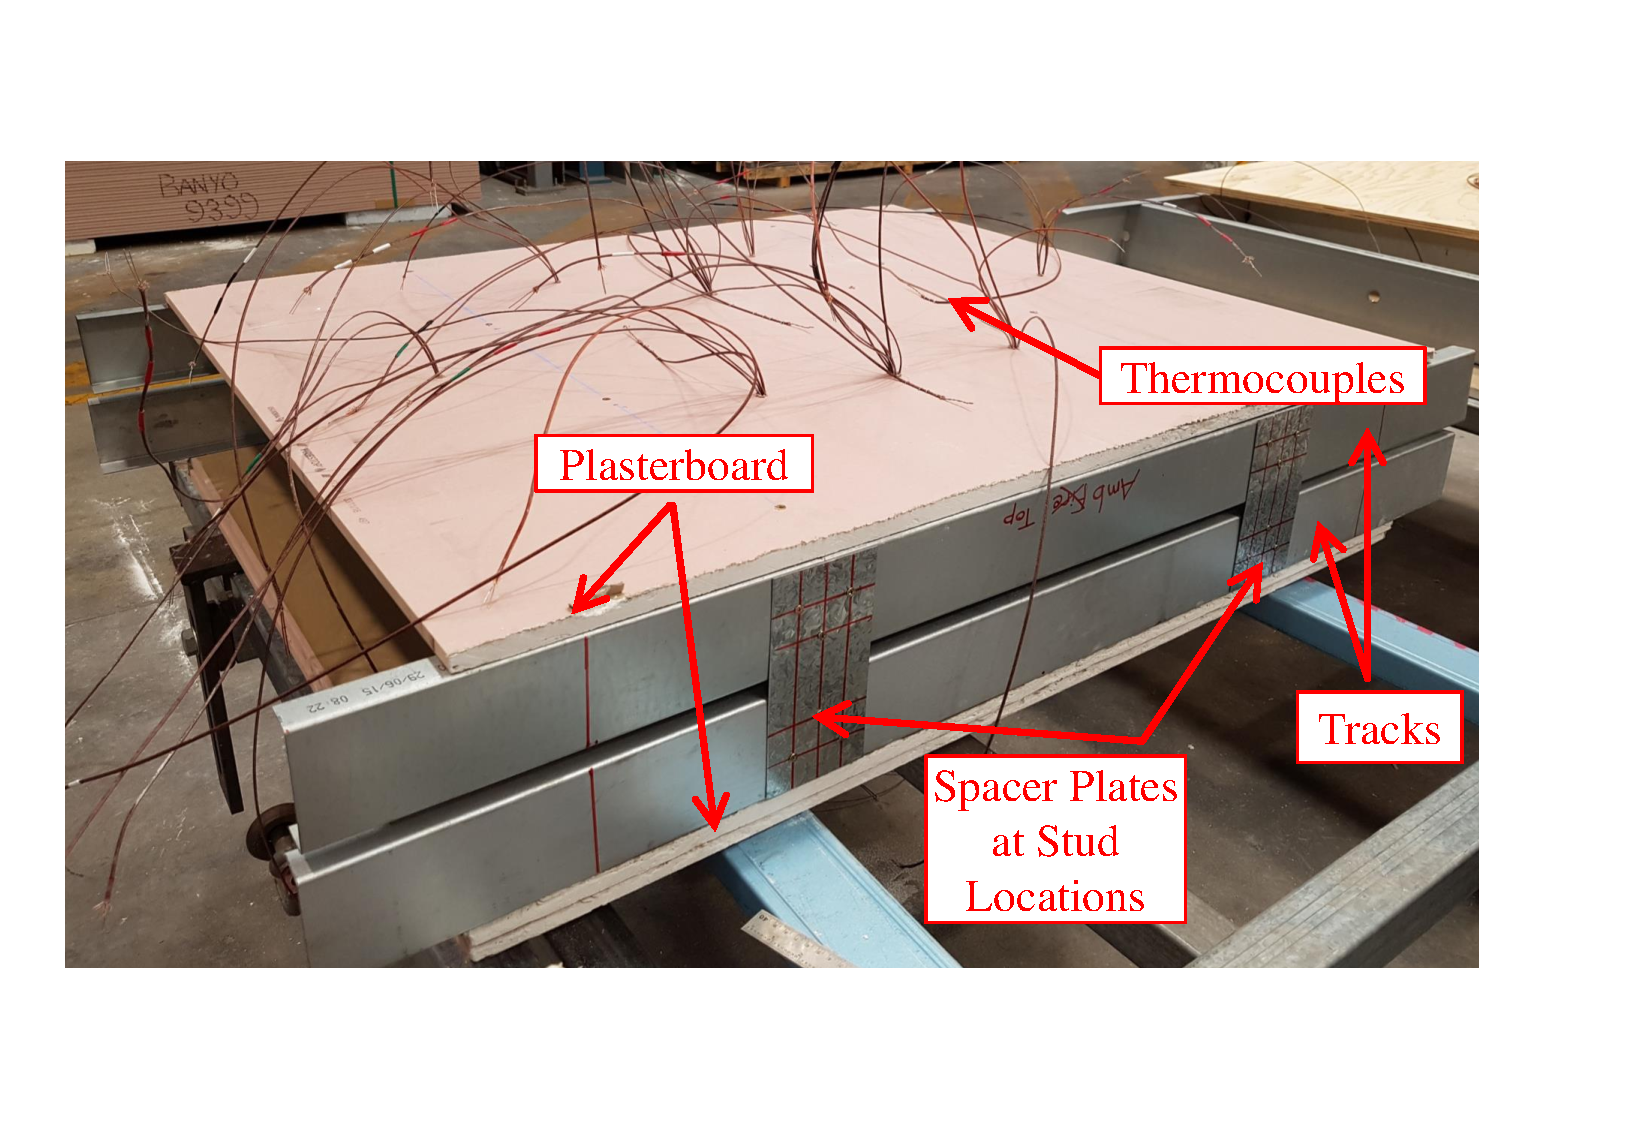
\includegraphics[width=7cm,height=6cm]{ST-specimen.pdf} & 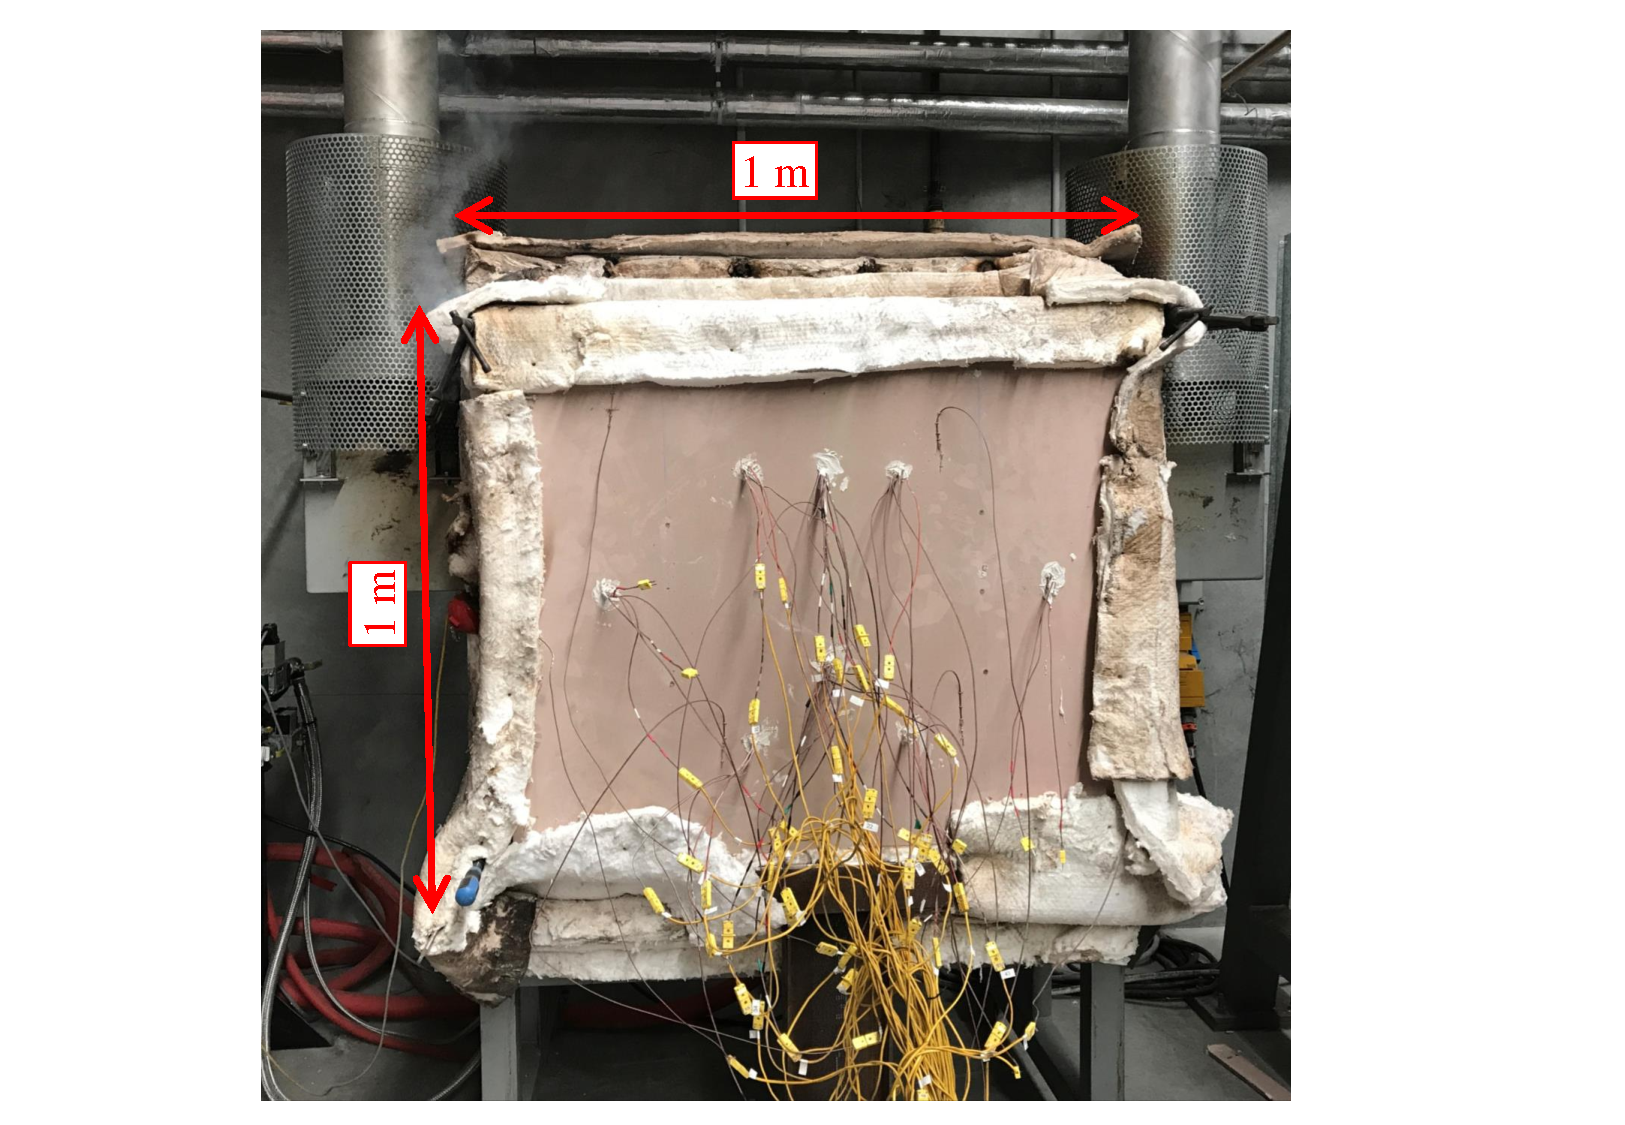
\includegraphics[width=7cm,height=6cm]{ST-setup.pdf} \\ 
			(a) & (b)  \\ 
		\end{tabular} 
		\caption{Plasterboard and stud time-temperature curves of Test-T1 (a) Average plasterboard temperature (b) Stud3 temperature}
		\label{fig:ST-setup}
\end{figure}
\begin{figure}[!htbp]
	\centering
		\begin{tabular}{cc}
			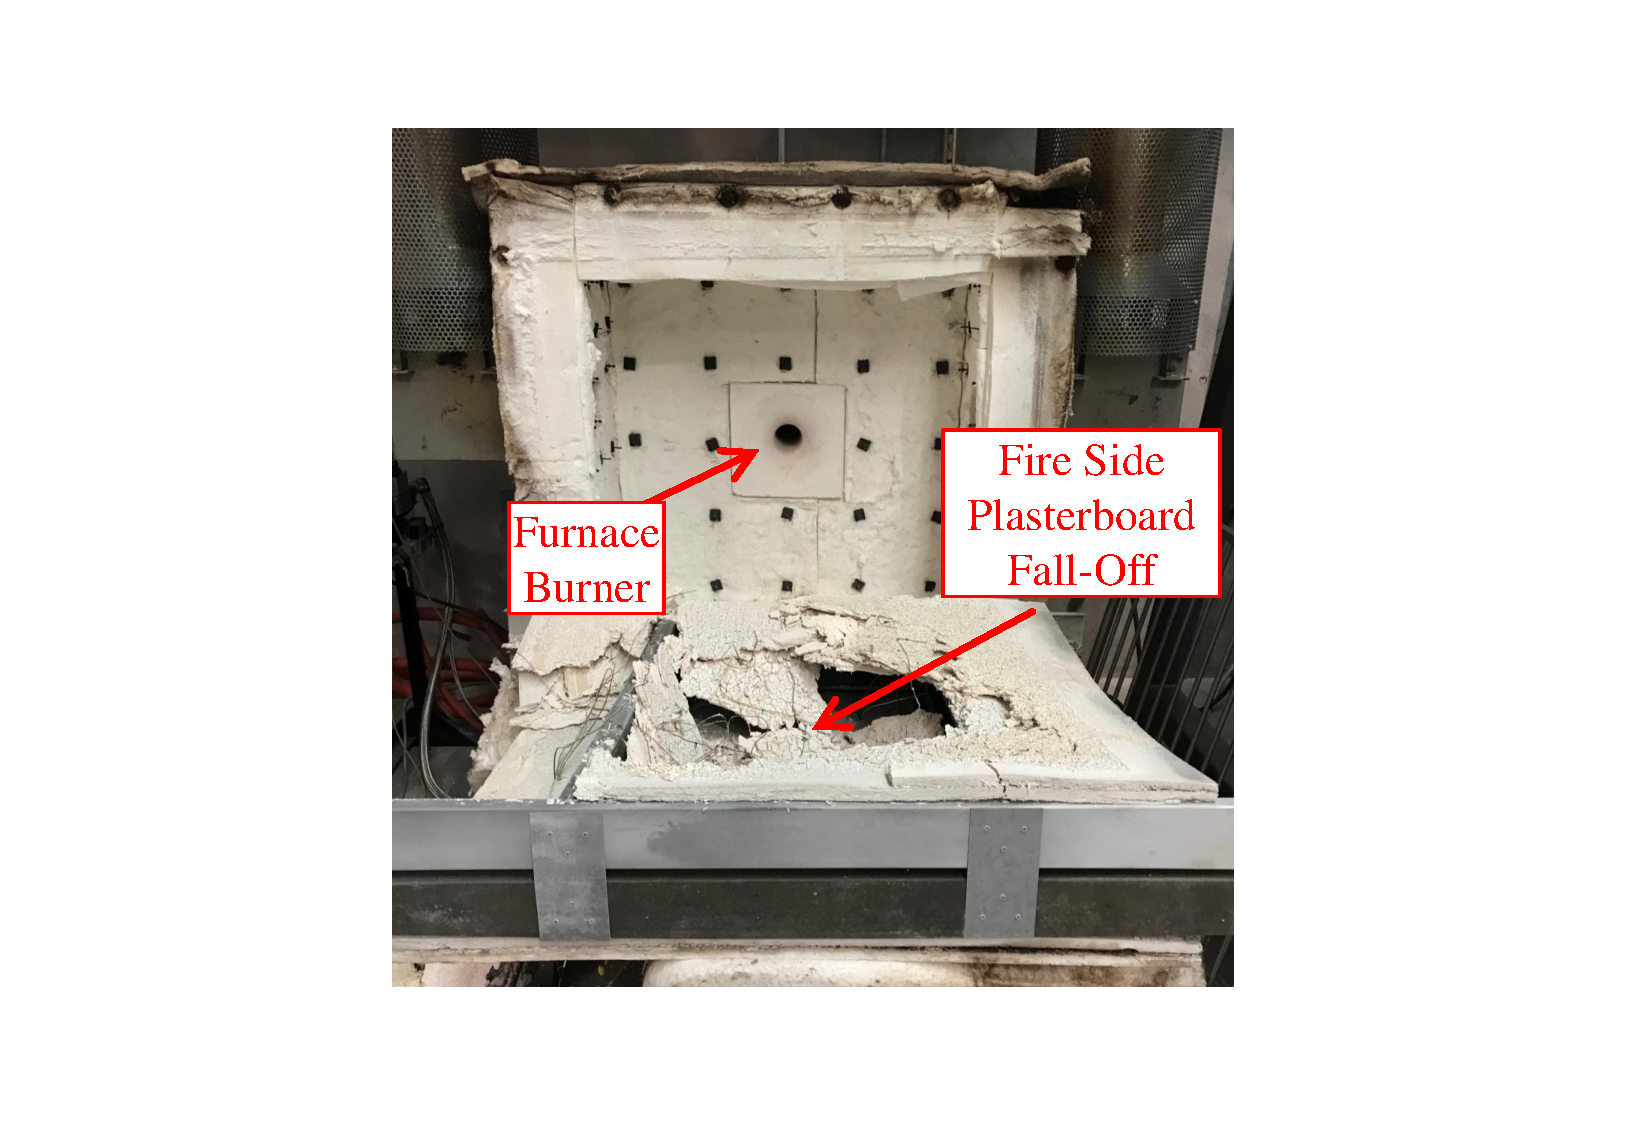
\includegraphics[width=7cm,height=6cm]{ST-failure1.pdf} & 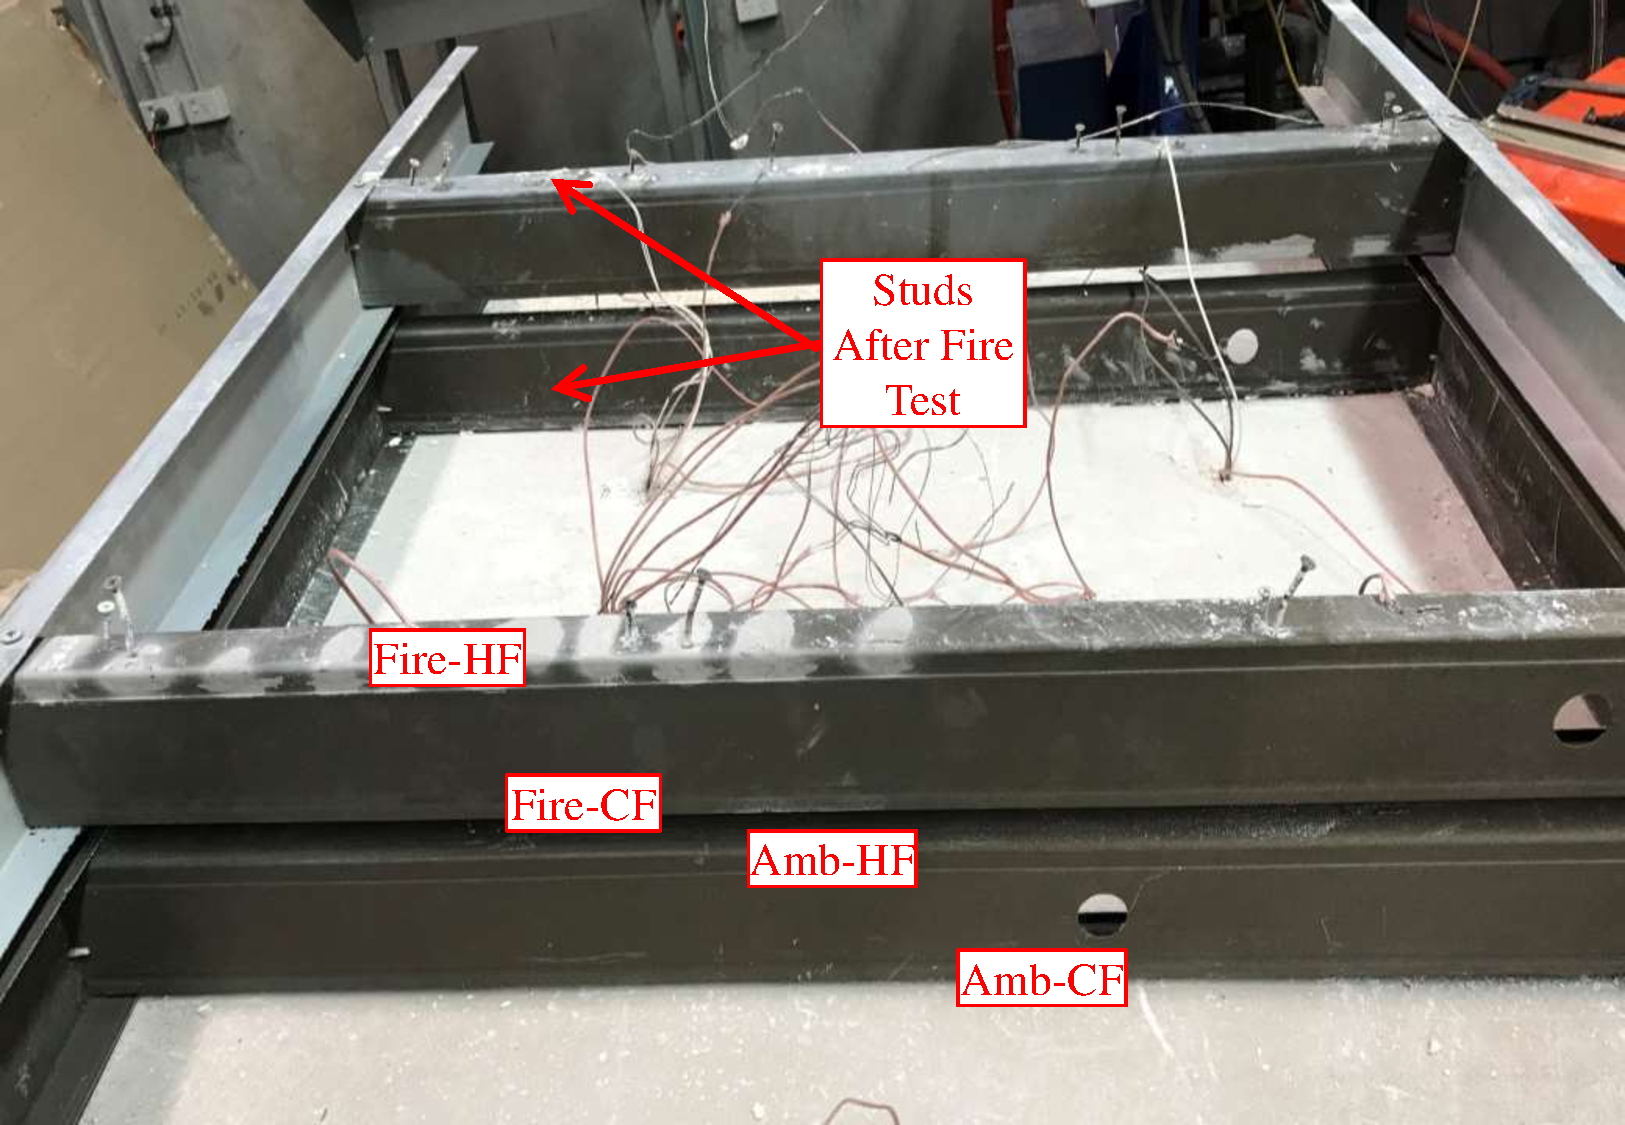
\includegraphics[width=7cm,height=6cm]{ST-failure2.pdf} \\ 
			(a) & (b)  \\ 
		\end{tabular} 
		\caption{Plasterboard and stud time-temperature curves of Test-ST1 (a) Average plasterboard temperature (b) Stud2 temperature}
		\label{fig:ST-failure}
\end{figure}

Test wall was clamped to the small furnace and ceramic insulation was wrapped around the specimen to prevent heat loss around the sides during fire test as shown in \Cref{fig:ST-setup}(b). The test wall was then subjected to AS 1530.4 standard fire curve based on ISO 834 and the fire test was conducted. Mild smoke was noticeable from 30 min till 80 min of the fire test representing the calcination of fire side plasterboard. Also, water droplets were visible on the clamps used for attaching the test wall to the furnace at certain intervals. The fire test was conducted for 176 min after which the test was stopped due to insulation failure criteria where the temperatures on the ambient side at the top left corner exceeded the limiting temperature of 200\degree C. Post fire test investigation revealed severe plasterboard fall-off on fire side resulting in sudden increase in temperature on the ambient side at a particular point. However, the thermocouple measured ambient side plasterboard surface (Pb4) temperatures were well below 100\degree C till the end of fire test. No deformation in the studs were observed as shown in \Cref{fig:ST-failure} as this was a non-load bearing test with shorter stud sections. The plasterboard fall-off was due to the hot air from the furnace concentrated on a small area of the test frame in small-scale fire test for a longer time period.

\subsection{Small-Scale Fire Test - Results and Discussion}

The small-scale fire test results showing the time-temperature evolution of the plasterboards and studs are shown in \Cref{fig:ST1-PB&Stud}(a). Fire side plasterboard interface temperatures (Pb1-Pb2)was flat for the initial 20 min after which a steep rise in the curve was noticed. This was followed by a plateau region from 70 min to 120 min after which the curve increased gradually till the end of fire test. A sudden increase in the time-temperature curves were observed in all the plasterboard surfaces indicating plasterboard fall-off. The possibility of joint open cannot happen as the specimen did not have any plasterboard joints. This unique behaviour in the time-temperature curve is also reflected on the fire side cavity (Pb2) and the ambient side cavity surface (Pb3). However, ambient side plasterboard interface surface (Pb3-Pb4) recorded temperatures less than 100\degree C till 150 min and reaching a maximum of 280\degree at the end of fire test. The stud time-temperature curves are plotted in \Cref{fig:ST1-PB&Stud}(b).  
\begin{figure}[!htbp]
	\centering
		\begin{tabular}{cc}
			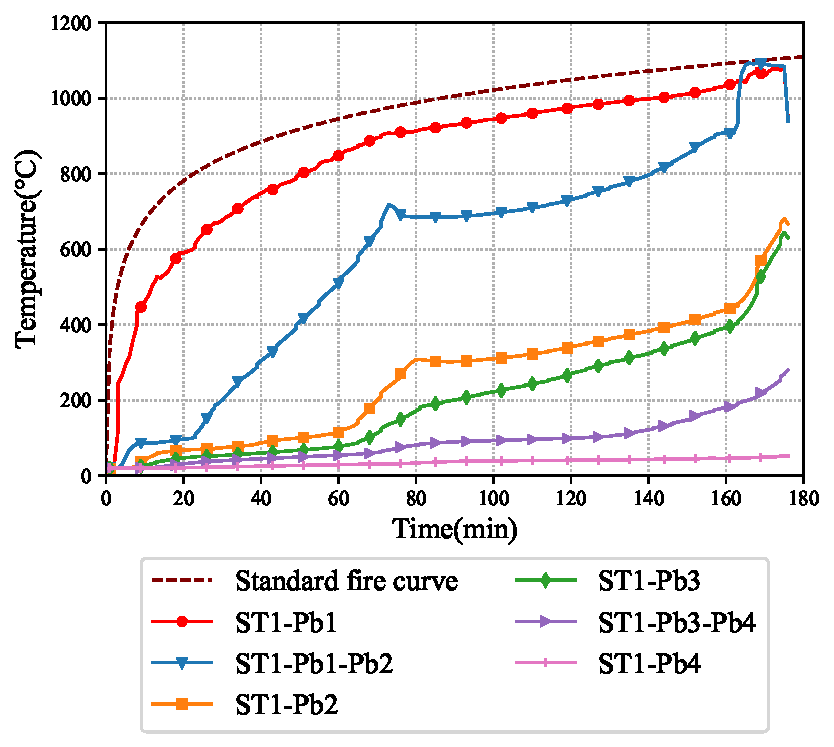
\includegraphics[width=7cm,height=6cm]{ST1-Average-Pb.pdf} & 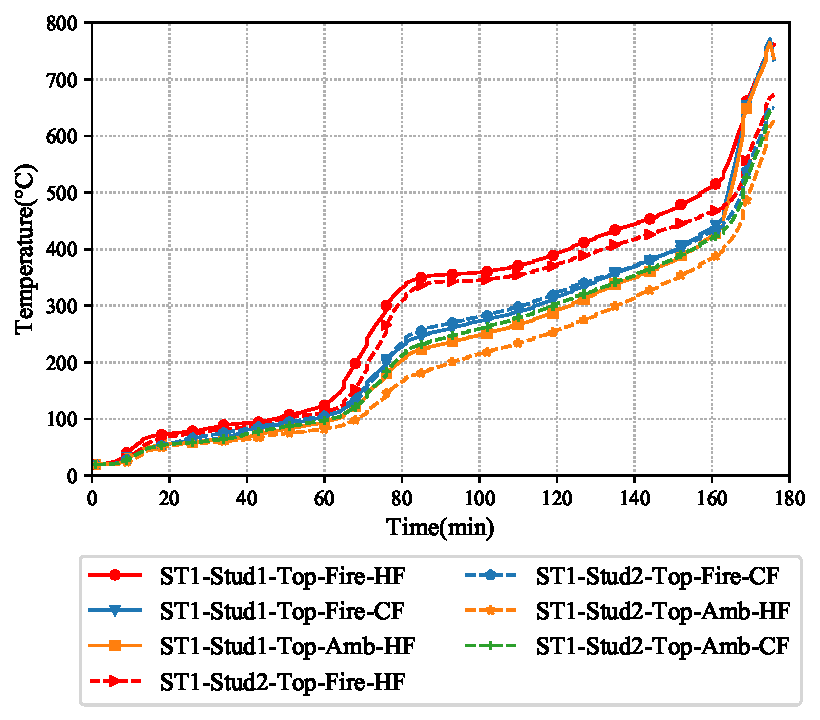
\includegraphics[width=7cm,height=6cm]{ST1-Stud1-2-Top.pdf} \\ 
			(a) & (b)  \\ 
		\end{tabular} 
		\caption{Plasterboard and stud time-temperature curves of Test-ST1 (a) Average plasterboard temperature (b) Stud2 temperature}
		\label{fig:ST1-PB&Stud}
\end{figure}

The hot and cold flange temperatures of Stud1 and Stud2 recorded temperatures less than 200\degree C till 65 min of the fire test. A sudden increase in the time-temperature curve of the fire side hot and cold flanges (ST1-Stud1 and Stud2-Top-Fire-HF and CF) was noticed after 65 min, after which the curve exhibits a gradual increase correlating with the corresponding plasterboard temperatures. However the plateau region was not significantly observed in the stud time-temperature curves. The sudden increase in the hot flange temperatures proves the presence of plasterboard fall-off in the fire test. The cold flange temperatures were in close relation with the corresponding hot flange temperatures as shown in \Cref{fig:ST1-PB&Stud}. It is to note that the difference in temperature gradient between the fire the cold flange (ST1-Stud1 and Stud2-Top-Fire-CF) and the ambient side hot and cold flanges (ST1-Stud1 and Stud2-Top-Amb-HF and CF) were small in comparison with the fire side hot and cold flanges. This indicates the delayed heat transfer mechanism in wider cavity LSF walls. This is further investigated and discussed in the full-scale fire test section of this chapter.

\section{Full-scale Fire Test on Double Stud LSF Walls}
\subsection{Fire Test Panel Details}

To investigate the heat transfer mechanism in detail a series of fire tests were conducted on the complex LSF wall system. The test wall panels were constructed with frame dimensions of 3 m \(\times\) 3 m as shown in \Cref{fig:ds-elevation}. Total of 10 full-scale fire tests were conducted for the experimental study. Lipped Channel Sections (LCS) were used as studs and Unlipped Channel Sections (UCS) were used as tracks. Intermittent lateral restraints using 0.55 mm thick noggings located at 1000 mm intervals were provided for some of the fire tests. Stud thickness, cavity depth, load ratio and cavity insulations were the variable parameters and are detailed in \Cref{tab:test-specimens}. G550 steel (minimum yield strength of 550 MPa) was used for all the fire tests.  The studs, tracks and noggings were connected using Buildex M6.0 \(\times\) 15 GX Ca smooth top GA point steel frame and truss screws with studs at 600 mm centres. A 20 mm gap was maintained between the two rows of steel frames by using 50 mm x 200 mm spacer plates. 
\begin{table}[!htbp]
	\begin{threeparttable}
		\centering
			\caption{Fire test panel details}
				\begin{tabular}{ccccccc}
					\toprule
					\multicolumn{1}{m{2.4em}}{\centering{Test Name}} & 
					\multicolumn{1}{m{5.6em}}{\centering{Description}} & 
					\multicolumn{1}{m{2.85em}}{\centering{Stud Depth (mm)}} & 
					\multicolumn{1}{m{2.85em}}{\centering{Cavity Depth (mm)}} & 
					\multicolumn{1}{m{5em}}{\centering{Stud Thickness (mm)}} & 
					\multicolumn{1}{m{5em}}{\centering{Cavity Insulation}} &
					\multicolumn{1}{m{3em}}{\centering{Loading Ratio}}\\
					\midrule
					T1  & Double Stud & 90 & 200 & 0.95 & No & 0.4 \\
					T2  & Double Stud & 90 & 200 & 0.75 & No & 0.4 \\
					T3  & Double Stud & 90 & 200 & 0.75 & No & 0.6 \\
					T4  & Double Stud & 70 & 160 & 0.95 & No & 0.4 \\
					T5  & Double Stud & 90 & 200 & 0.95 & Both\(^+\) & 0.4 \\
					T6\(^*\)  & Double Stud & 90 & 200 & 0.95 & Both\(^+\) & 0.4 \\
					T7  & Double Stud & 90 & 200 & 0.95 & Ambient\(^{++}\) & 0.4 \\
					T8  & Shaftliner & 90 & 196 & 0.75 & No & NLB\\
					T9  & Staggered Stud & 90 & 150 & 0.75 & No & NLB\\
					T10  & Staggered Stud & 90 & 150 & 0.95 & Full\(^{*+}\) & 0.4 \\
					\bottomrule
				\end{tabular}%
				\label{tab:test-specimens}%
					\begin{tablenotes}
						\small
						\item \textit{\(^*\) Repeat of Test-T5}
						\item \textit{\(^+\) Cavity insulation on both stud rows}
						\item \textit{\(^{++}\) Cavity insulation on ambient stud rows only}
						\item \textit{\(^{*+}\) Cavity insulation staggered alongside the studs}
						\item \textit{NLB - Non-Load Bearing}
					\end{tablenotes}
		\end{threeparttable}
\end{table}%
\begin{figure}[!htbp]
	\centering
				\begin{tabular}{cc}
			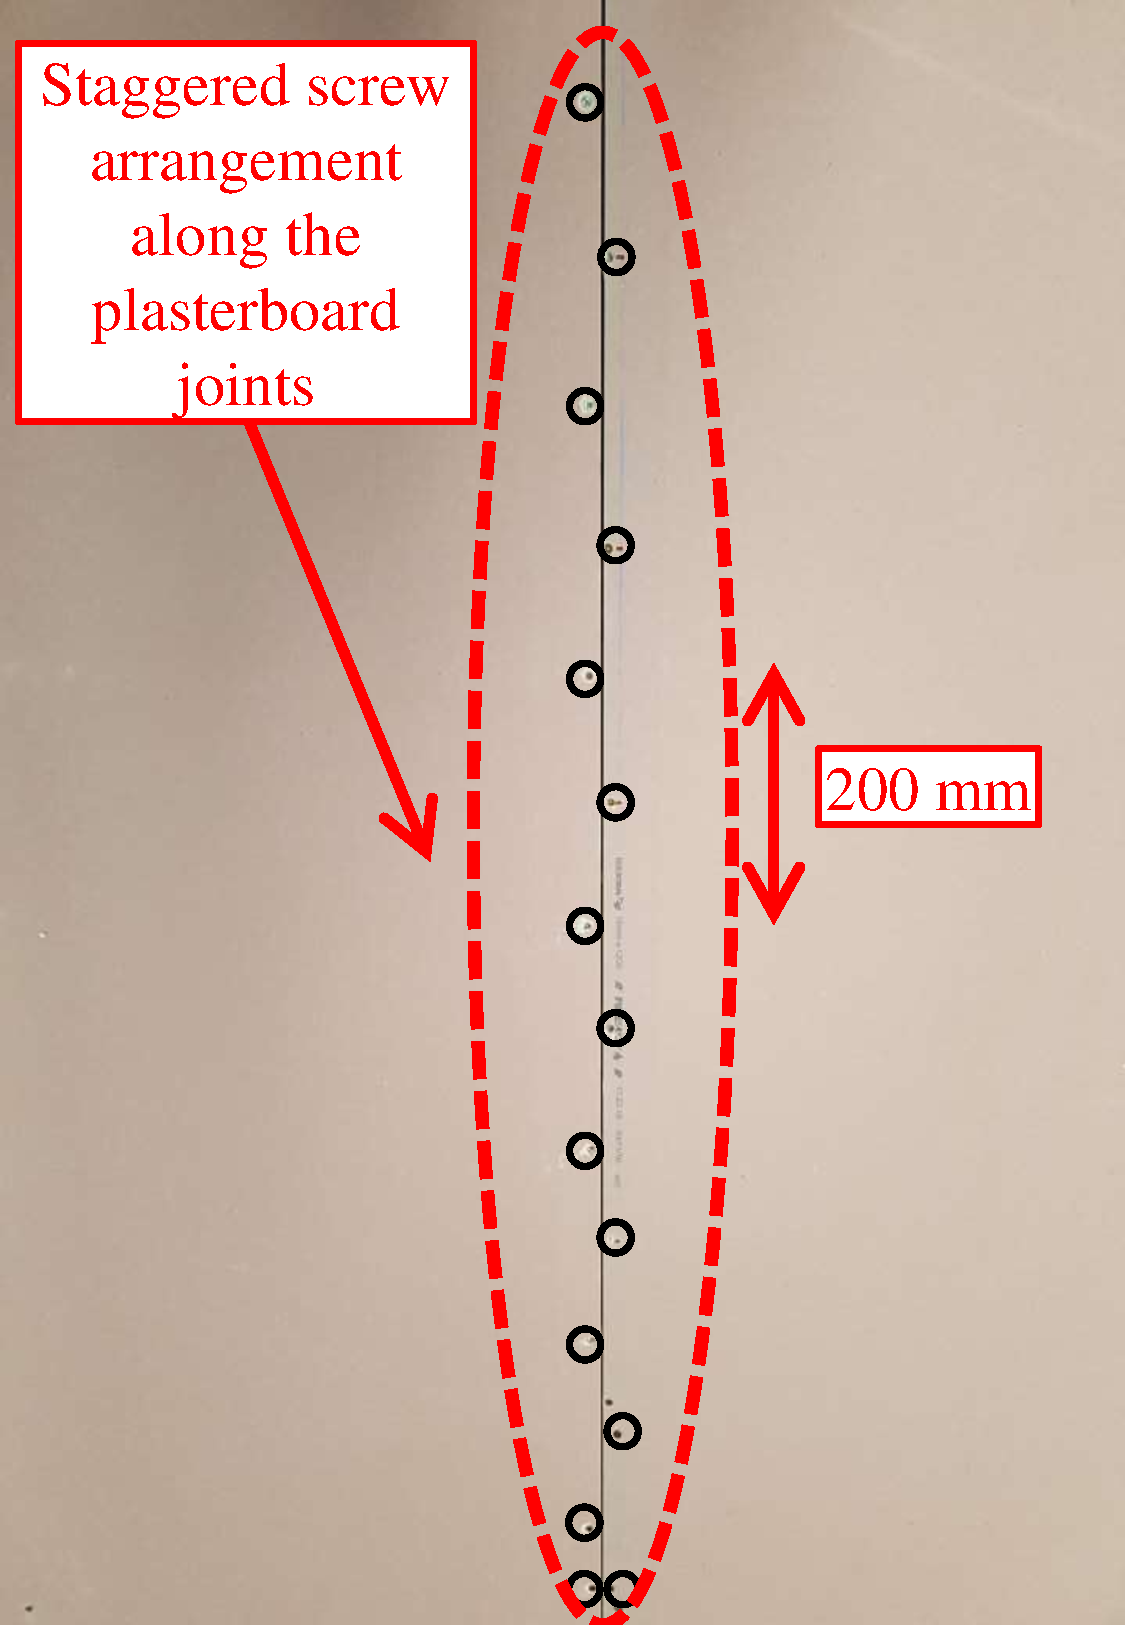
\includegraphics[width=4.5cm, height=6.5cm]{pb_screw-staggered.pdf} & 
			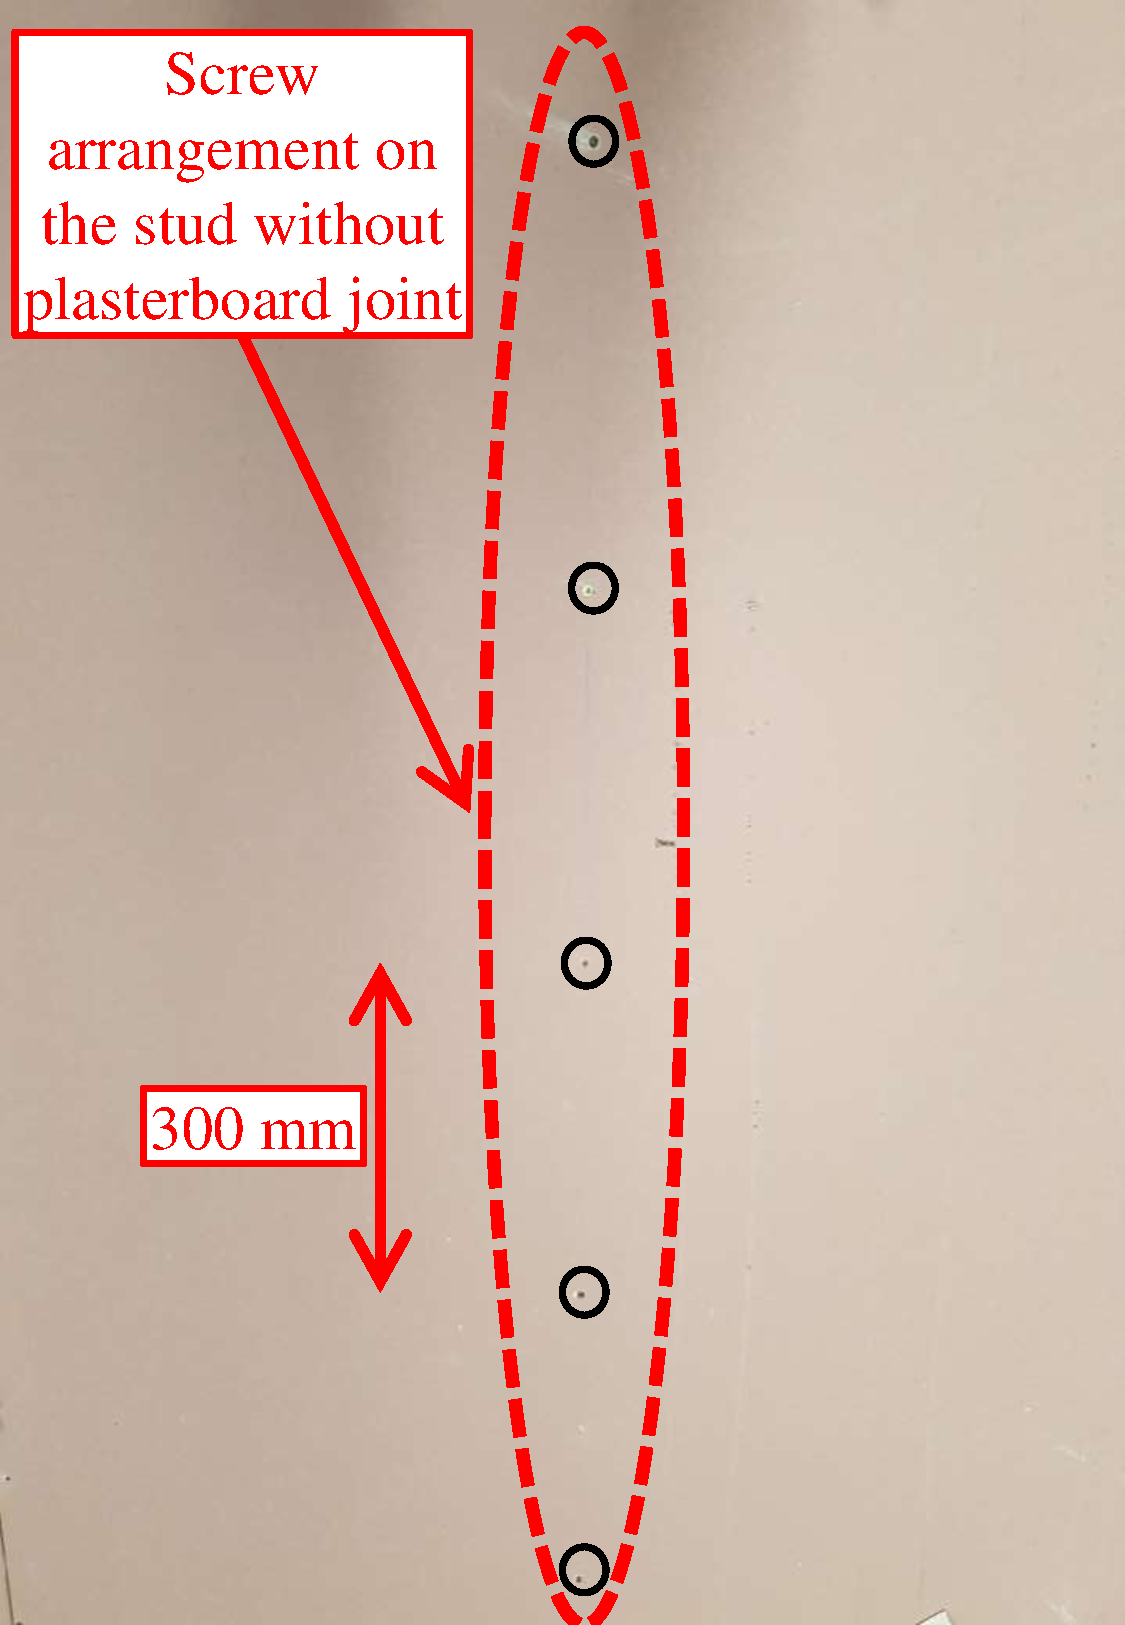
\includegraphics[width=5cm, height=6.5cm]{pb_screw-linear.pdf} \\
			(a) & (b) \\ 
		\end{tabular} 
		\caption{Location of plasterboard screws}
		\label{fig:screw}
		\fontsize{10}{1}\textit{Note : All dimensions are in mm.}
\end{figure}
\begin{figure}[!htbp]
	\centering
		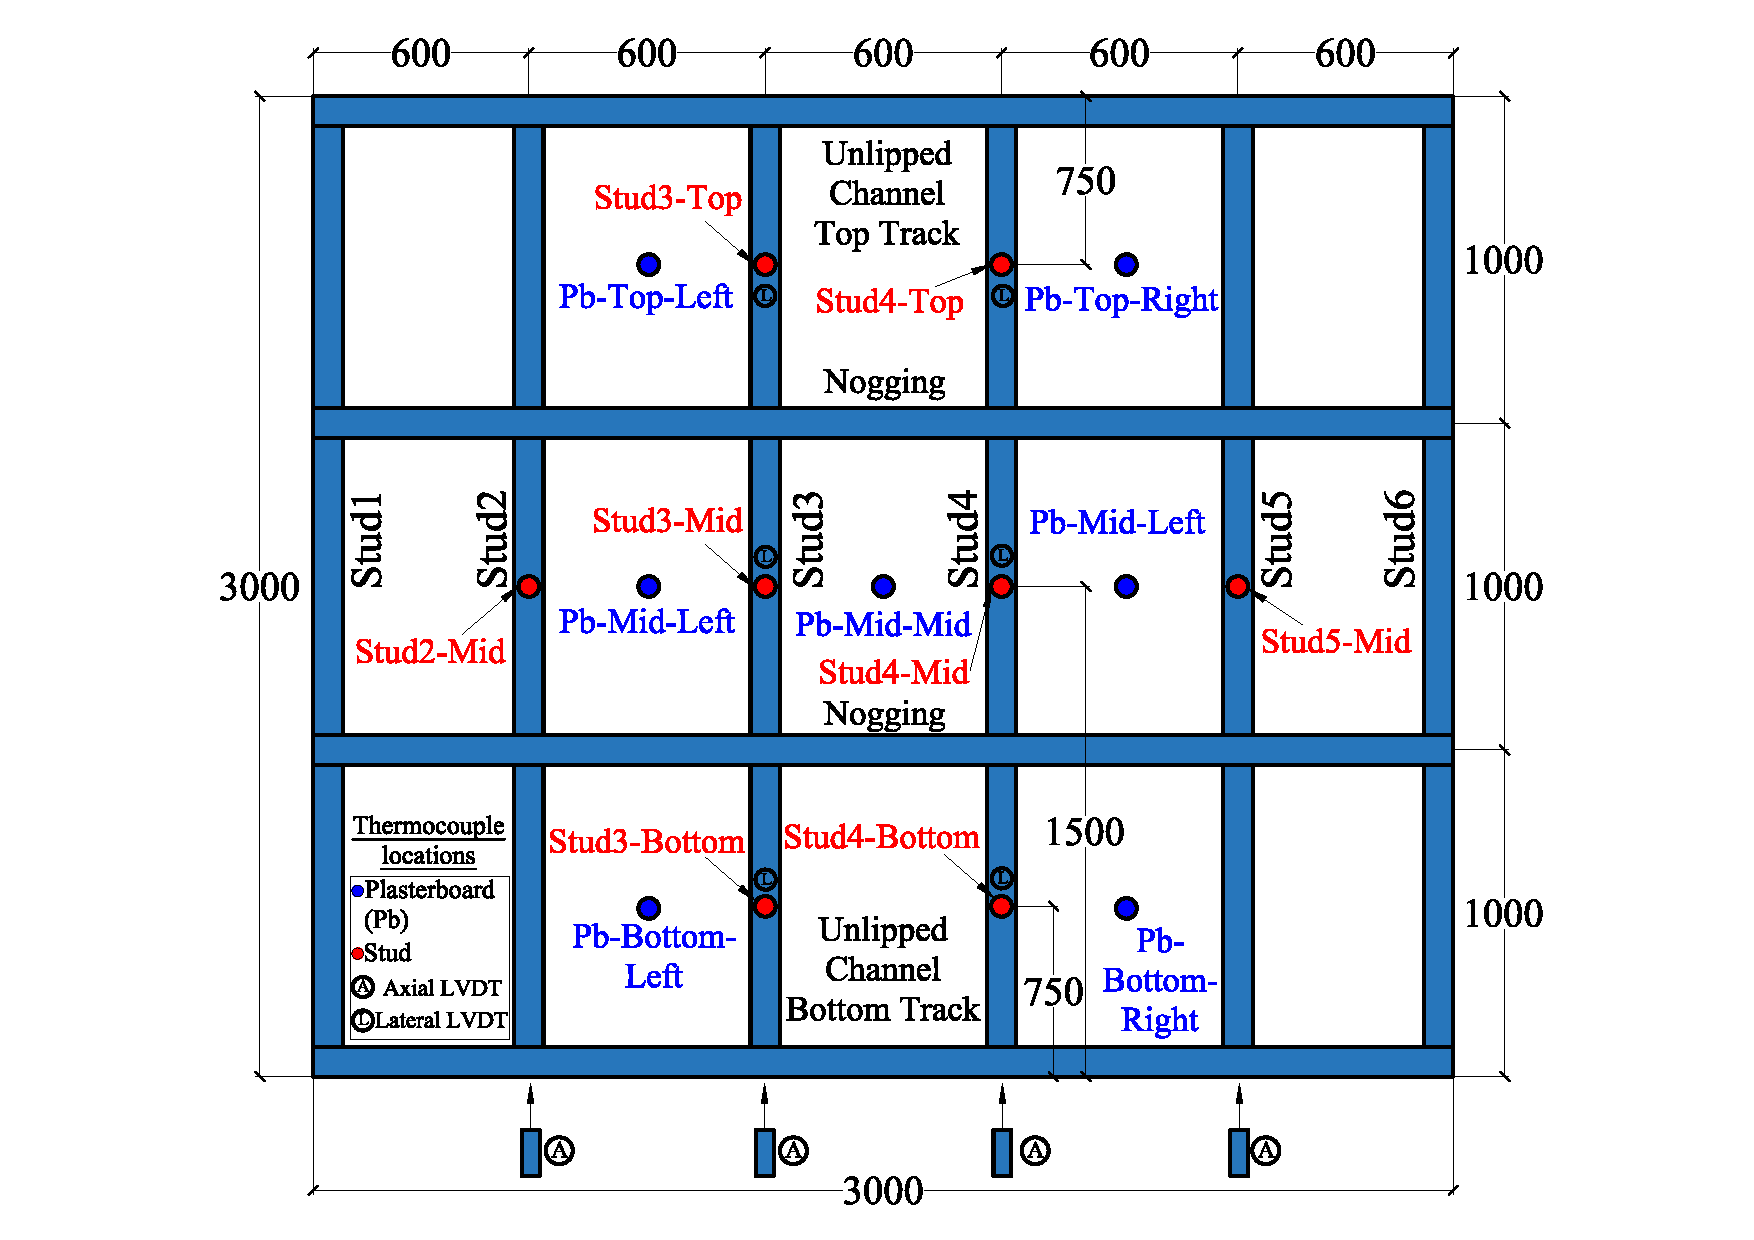
\includegraphics[width=10cm, height=9cm]{ds-elevation.pdf}
		\caption{Elevation of Double Stud LSF Wall Panel}
		\label{fig:ds-elevation}
		\fontsize{10}{1}\textit{Note : All dimensions are in mm.}
\end{figure}

Two layers of 16 mm thick USG Boral Firestop gypsum plasterboards measuring 1200 \(\times\) 3000 mm were used as lining on both sides of the wall and were attached to the frames using D type 10 GA self-piercing screws at 300 mm spacing in all the fire tests. The first layer of plasterboard was attached using 32 mm long screws while the second layer was attached using 45 mm long screws. They were screw fastened only to the studs (not tracks). This is achieved by providing a 60 mm gap from the frame end to the screws when fixing the first plasterboard layer, while a 80 mm gap was provided for the second plasterboard layer. The first layer of plasterboard was placed vertically with two vertical joints and the second layer was placed horizontally with two horizontal joints. The screws were staggered at 200 mm near the plasterboard joints as shown in \Cref{fig:screw}. An edge distance of 10 to 15 mm was provided along all the plasterboard edges to prevent shearing of the screws from the plasterboard. USG Boral Basecoat 60 was used as the joint compound with 50 mm wide cellulose based joint tape. For fire designs, LSF walls are considered to be subjected to an axial compression load in the range of 40 to 60 \% of the ambient temperature load bearing capacity, i.e. load ratio (LR) of 0.4 to 0.6. Therefore, all the load bearing tests were conducted within this load range.

\subsection{Temperature Sensors and Displacement Transducers}

Sixty four thermocouples were used to measure the temperatures across the width and depth of the wall at various locations. Ten Linear Variable Displacement Transducers (LVDTs) were used to measure the axial shortening and lateral deflection of the wall as shown in \Cref{fig:furnace-specimen} (b). K-Type thermocouples that can measure the temperature within the range of -200\degree C to 1100\degree C were used. They were positioned at quarter heights (750 mm, 1500 mm, 2250 mm) along the stud height and on the fire exposed side (Pb1), fire side cavity (Pb2), ambient side cavity (Pb3) and the ambient side (Pb4) of plasterboards as shown in \Cref{fig:T1-plan,fig:ds-elevation}. For the plasterboard interfaces on the fire side (Pb1-Pb2) and ambient side (Pb3-Pb4) thermocouples were placed only at mid-height of the panel. For studs, thermocouples were placed on stud flanges at quarter heights (750 mm, 1500 mm, 2250 mm) of Studs 3 and 4 only whereas on Studs 2 and 5 they were placed only at mid-height (1500 mm) as shown in \Cref{fig:ds-elevation}. LVDTs were placed under Studs 2 to 5 to measure the axial displacements and at quarter heights along Studs 3 and 4 to measure the lateral deflections as shown in \Cref{fig:furnace-specimen}(b).
\begin{figure}[!htbp]
	\centering
		\begin{tabular}{cc}
		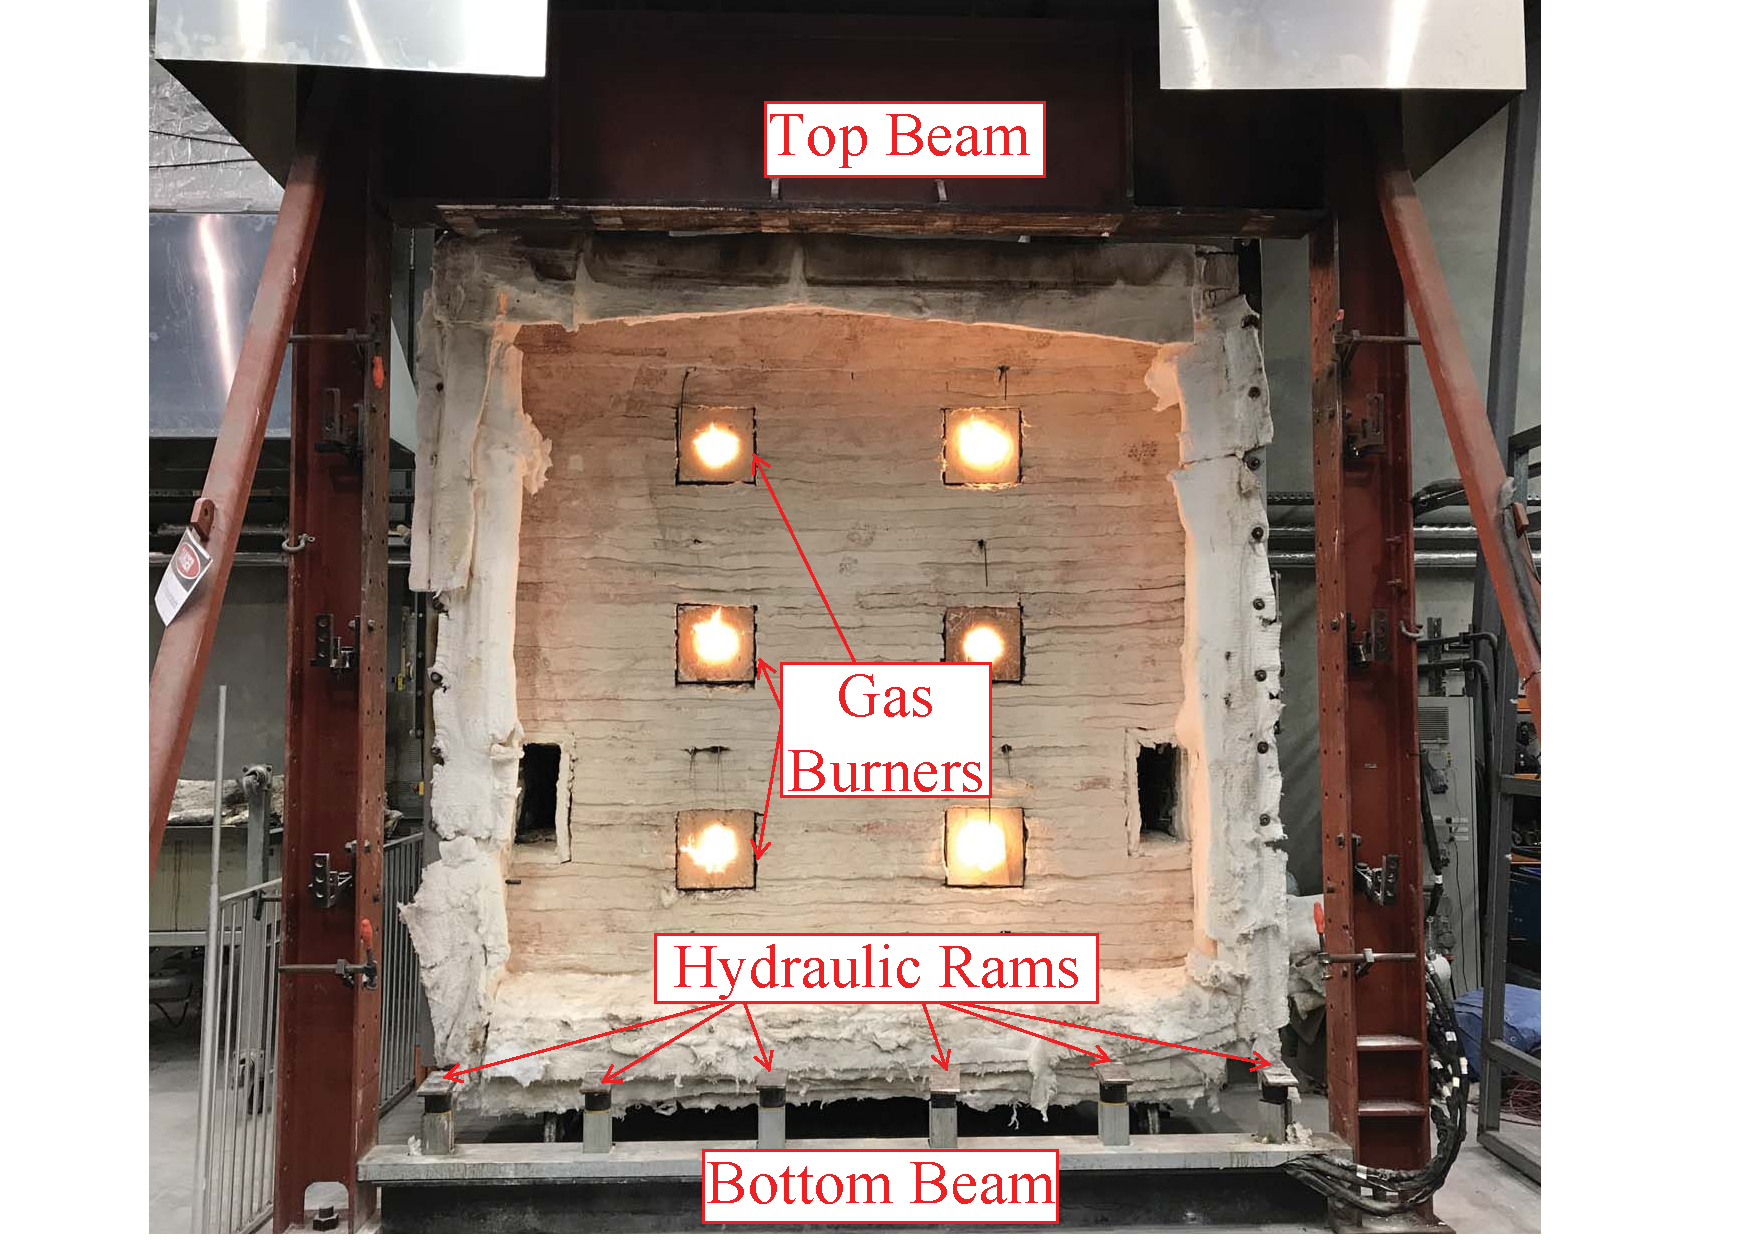
\includegraphics[width=6cm, height=6.5cm]{furnace2.pdf} &
		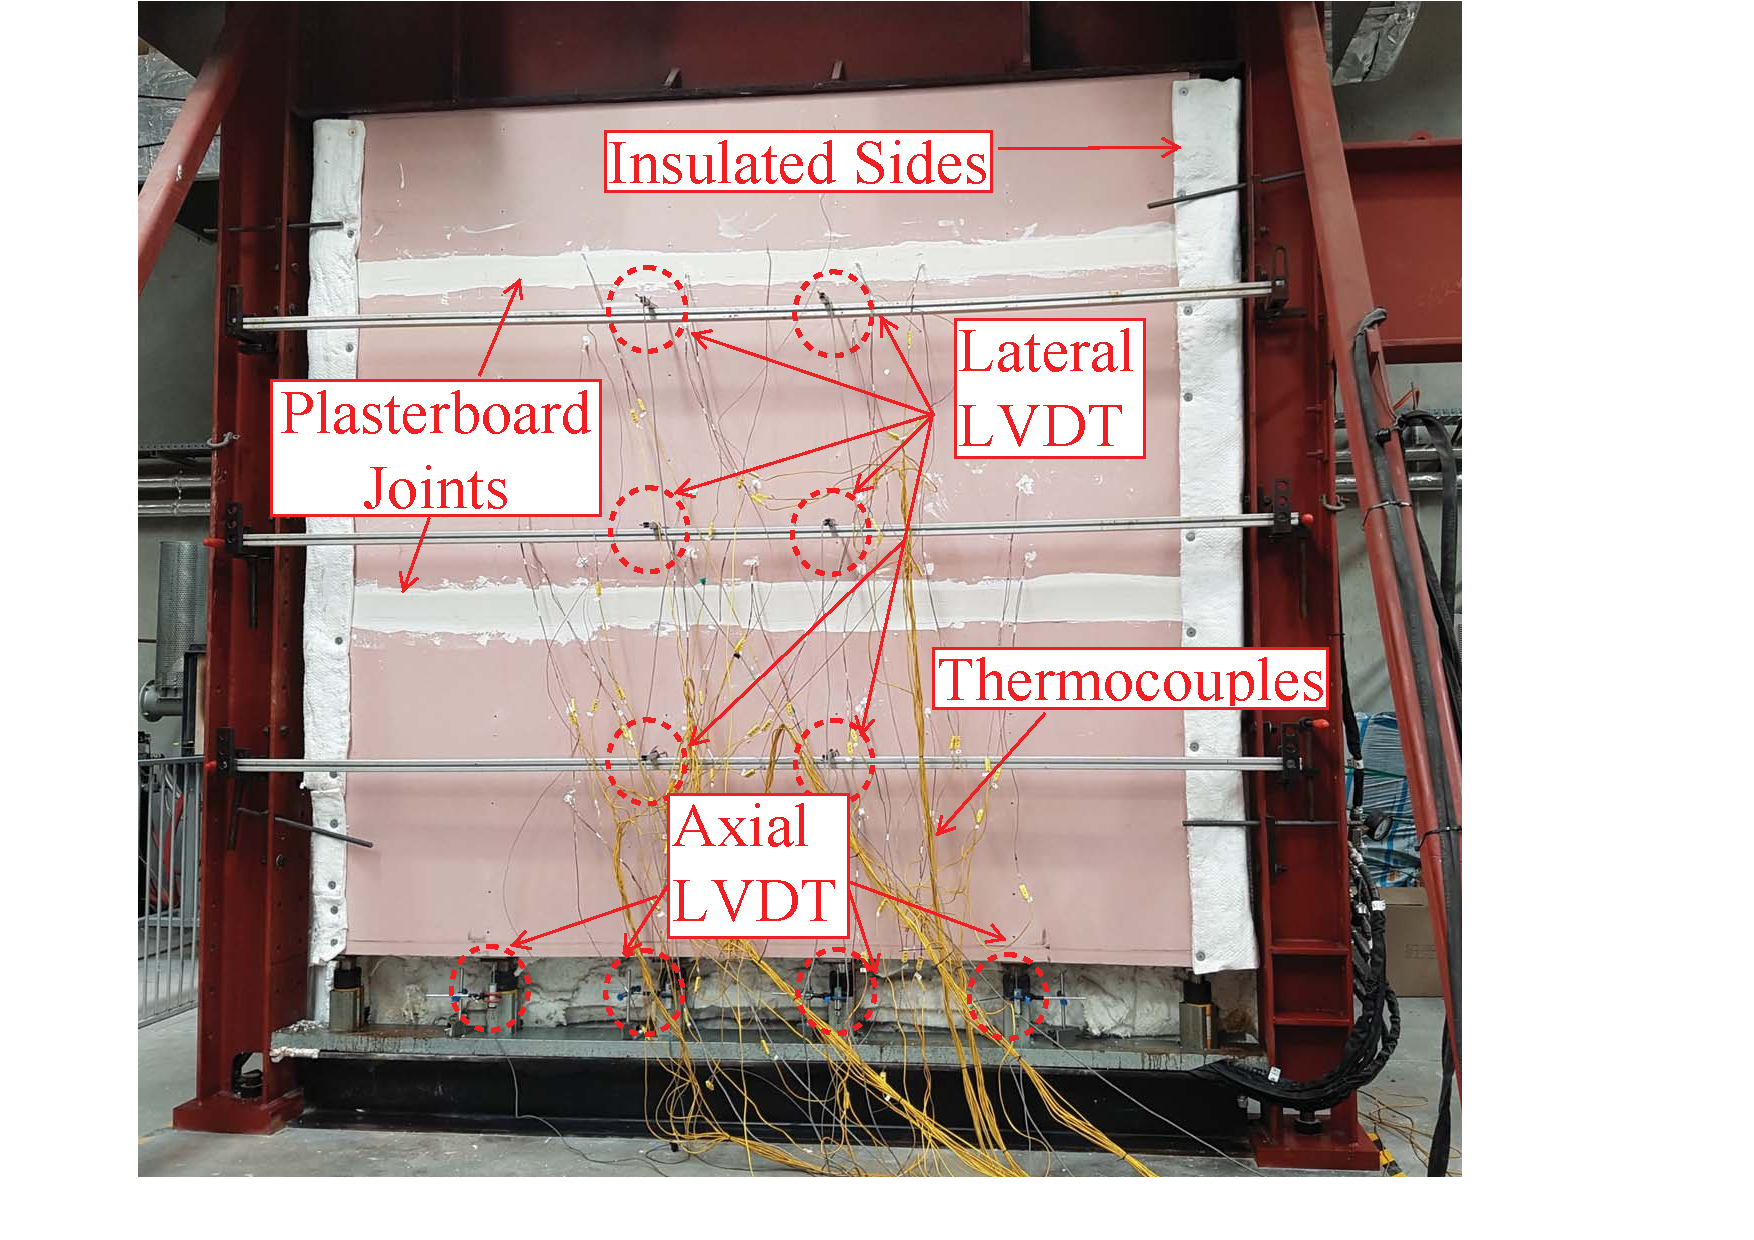
\includegraphics[width=6cm, height=6.5cm]{specimen2.pdf}\\
		(a) & (b)  \\ 
		\end{tabular} 
		\caption{Full scale fire test set-up (a) Furnace with pilot flame (b) Test panel}
		\label{fig:furnace-specimen}
\end{figure}

\subsection{Fire Test Set-up and Procedure}

Fire tests were conducted using a 3 \(\times\) 3 \(\times\) 0.4 m furnace consisting of six propane gas fuelled burners controlled by a EUROTHERM 3504 hybrid controller after applying the pre-determined axial compression loads using six hydraulic rams (\Cref{fig:furnace-specimen}(a)). The test rig was built with two universal columns (UC) bolted to the strong floor at the bottom and to a universal beam (UB) at the top. At the bottom end, a UB was fixed to the strong floor upon which six hydraulic rams were placed and connected to a pressure transducer. Once the wall panel was placed on the test rig an initial preload of 3 kN was applied to each stud to keep the wall panel in position before the fire test. The required load based on the load ratio was then applied to each stud by the hydraulic ram via a thick loading plate at the bottom end and was monitored through the data acquisition system. The test wall panel was then exposed to the standard fire time-temperature curve in AS 1530.4 \citet{StandardsAustral2014}. The test panel was insulated with ceramic fibre blankets along the edges to prevent any heat loss through the sides. The thermocouple and LVDT measurements were recorded using a Universal Data Acquisition (UDAQ) system with NI-LabView software until failure occurred. 

To easily identify the thermocouple and LVDT measurement locations, the fire and ambient side plasterboards are referred to as Pb1 and Pb4 while the internal plasterboards are referred to as Pb2 and Pb3 (\Cref{fig:T1-plan}). The interface between the two plasterboard layers on the fire side is referred to as Pb1-Pb2 while the interface between the ambient side plasterboard is referred to as Pb3-Pb4. The hot and cold flanges of single stud walls are referred as HF and CF. In double stud walls with two rows of stud, the hot and cold flanges of studs on the fire expose side are referred to as Fire-HF and Fire-CF whereas for those on the ambient side are referred to as Amb-HF and Amb-CF.

\section{Fire Test-T1}

Ambient capacity test conducted on the wall initially gave a stud capacity of 72.81 kN. Hence the fire test was conducted with studs loaded to 29.12 kN, i.e.,0.4 LR. The wall panel failed structurally after 176 min. No significant plasterboard fall-off was noticed during the fire test as shown in \Cref{fig:T1-failure} (a). The plasterboard cracked at 750 mm above the bottom track on the ambient side near the LVDT but no flames were visible as shown in \Cref{fig:T1-failure} (b). Local buckling of studs was the predominant mode of failure, which was clearly visible in Stud3 as shown in \Cref{fig:T1-failure} (c). It was significant only on the fire exposed row of studs. This is due to the effect of the 20 mm air gap between the two rows of studs.
\begin{figure}[htbp]
	\centering
	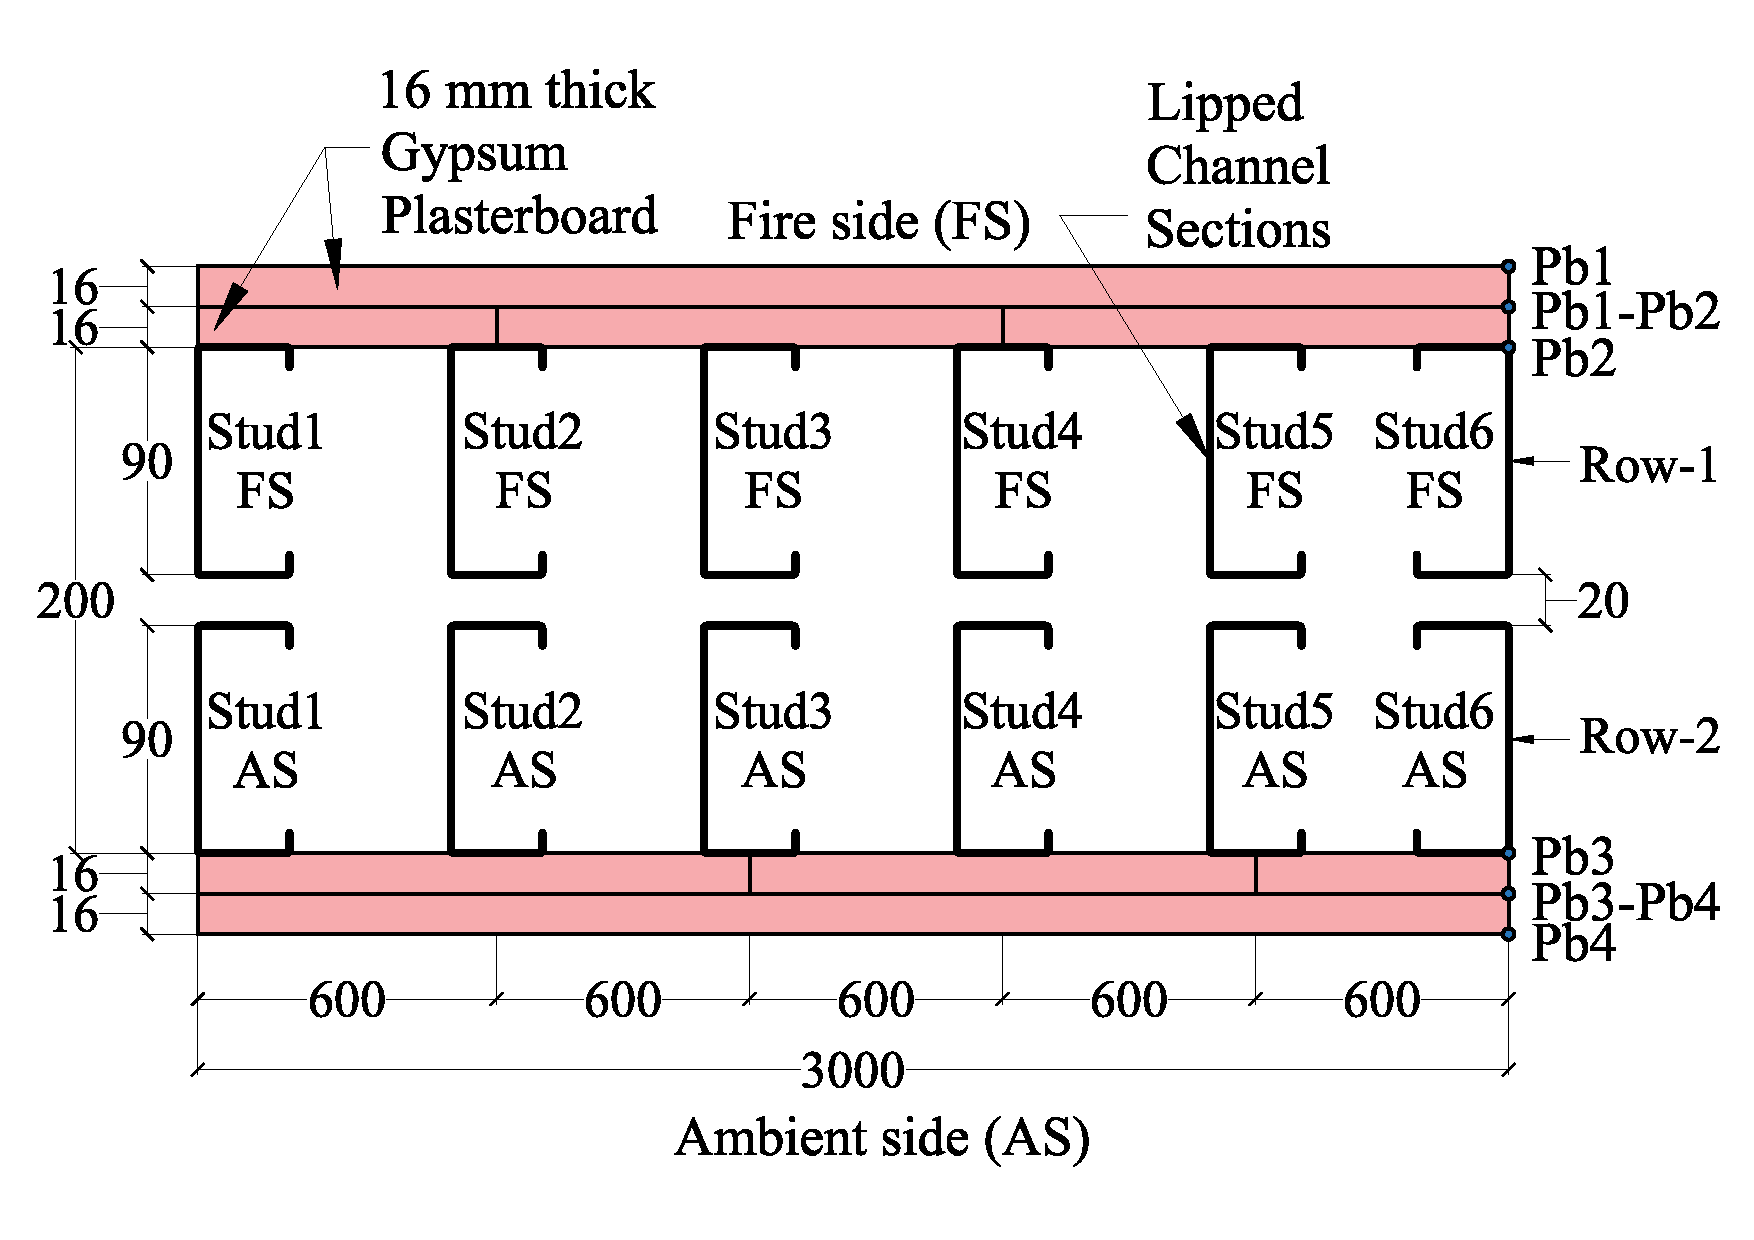
\includegraphics[width=8cm, height=5cm]{T1-plan.pdf}
	\caption{Plan view of Double Stud LSF Wall Panel}
	\label{fig:T1-plan}
	\fontsize{10}{1}\textit{Note : All dimensions are in mm.}
\end{figure}
\begin{figure}[htbp]
	\centering
		\begin{tabular}{ccc}
			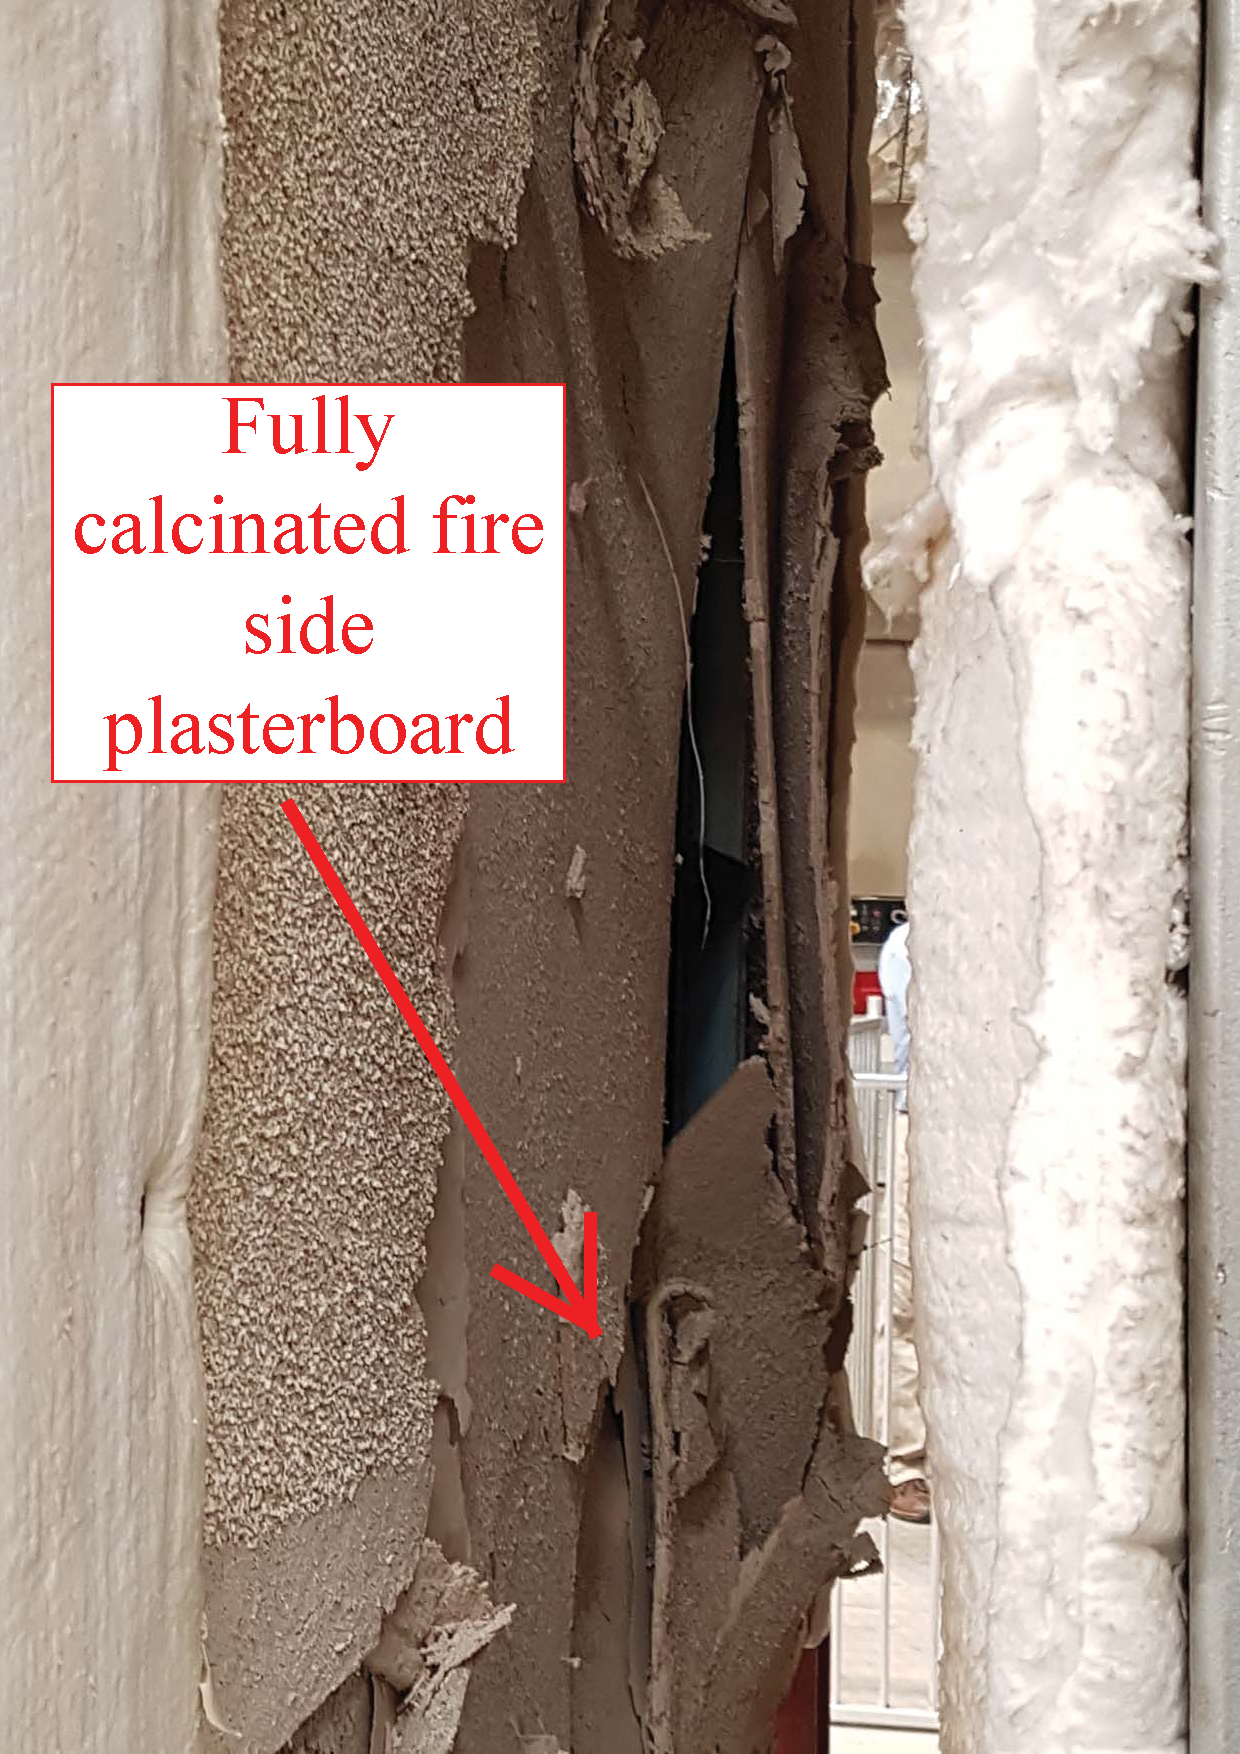
\includegraphics[scale=0.20]{T1-fire-side2.pdf} & 
			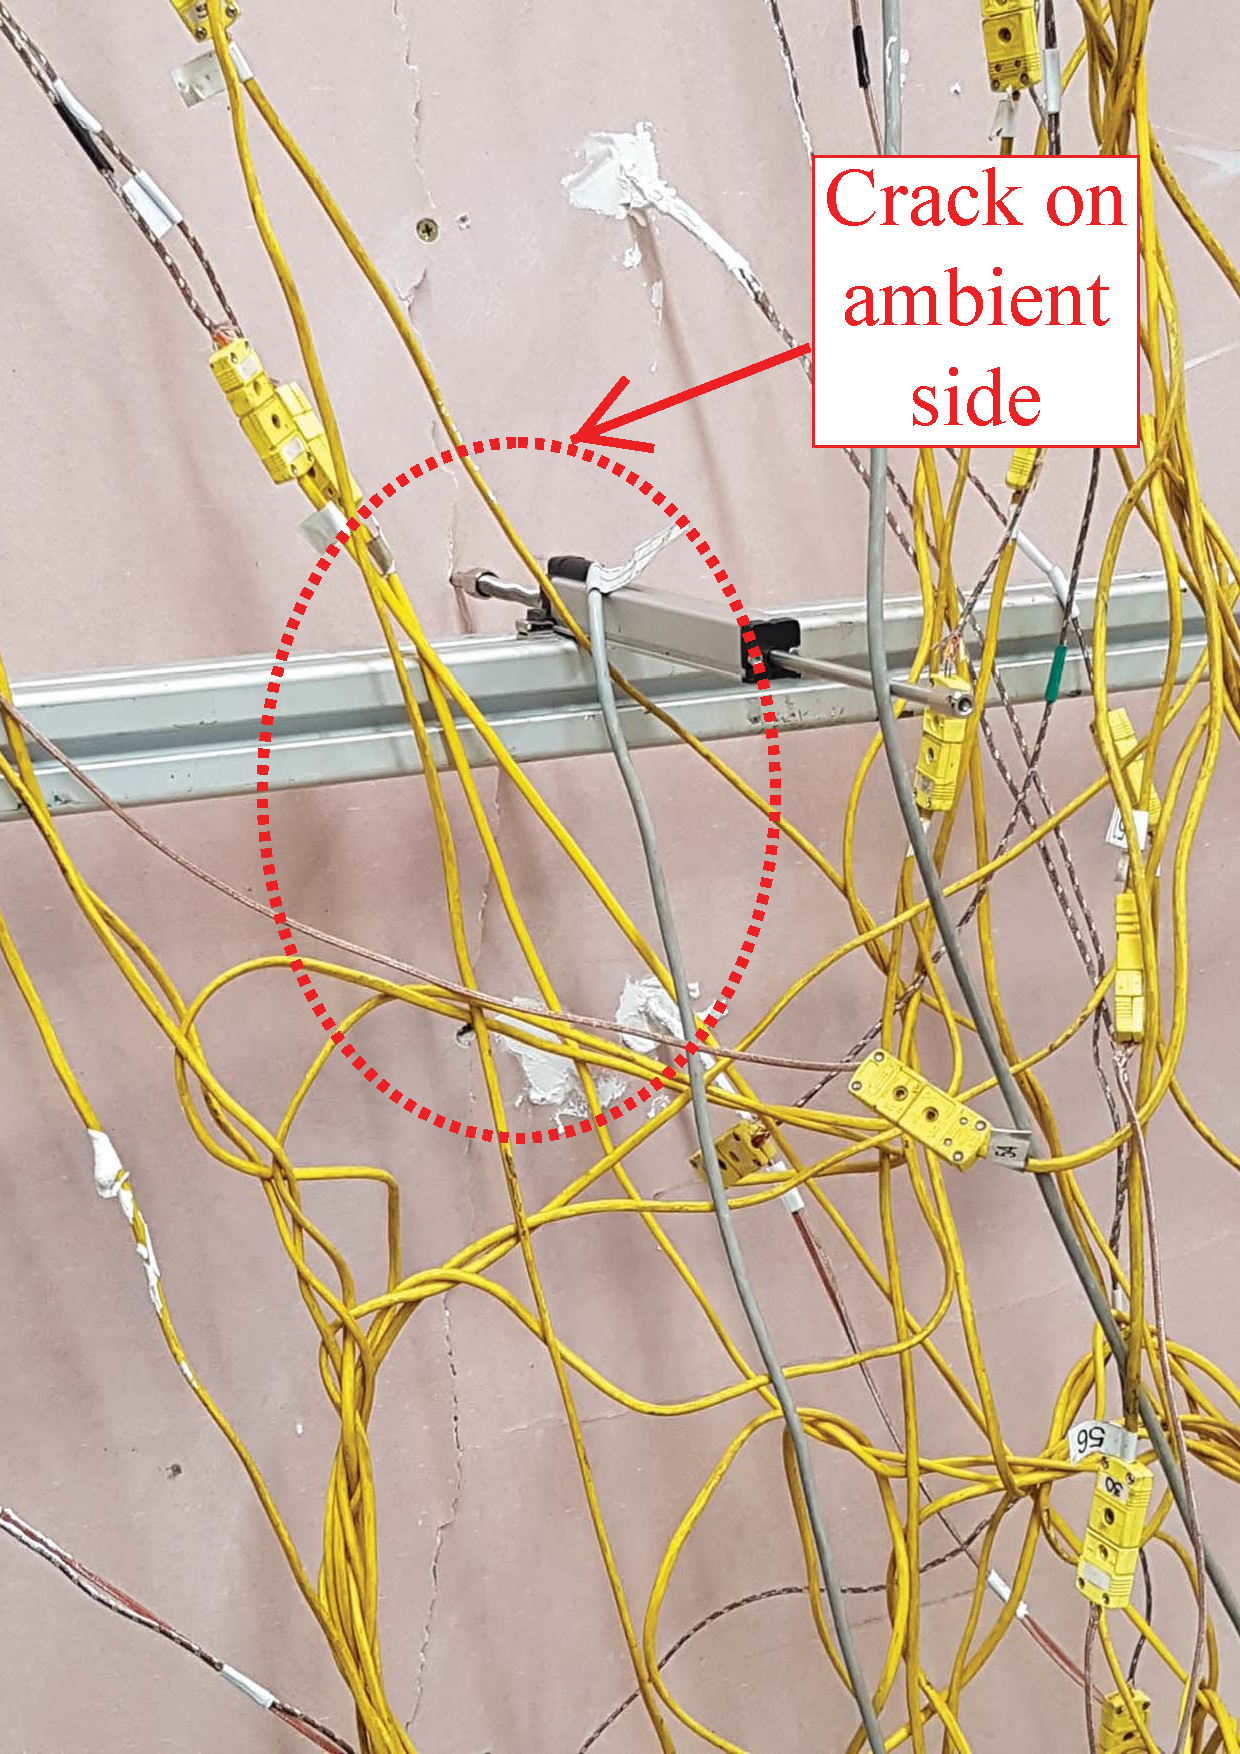
\includegraphics[scale=0.20]{T1-ambient-crack2.pdf} &
			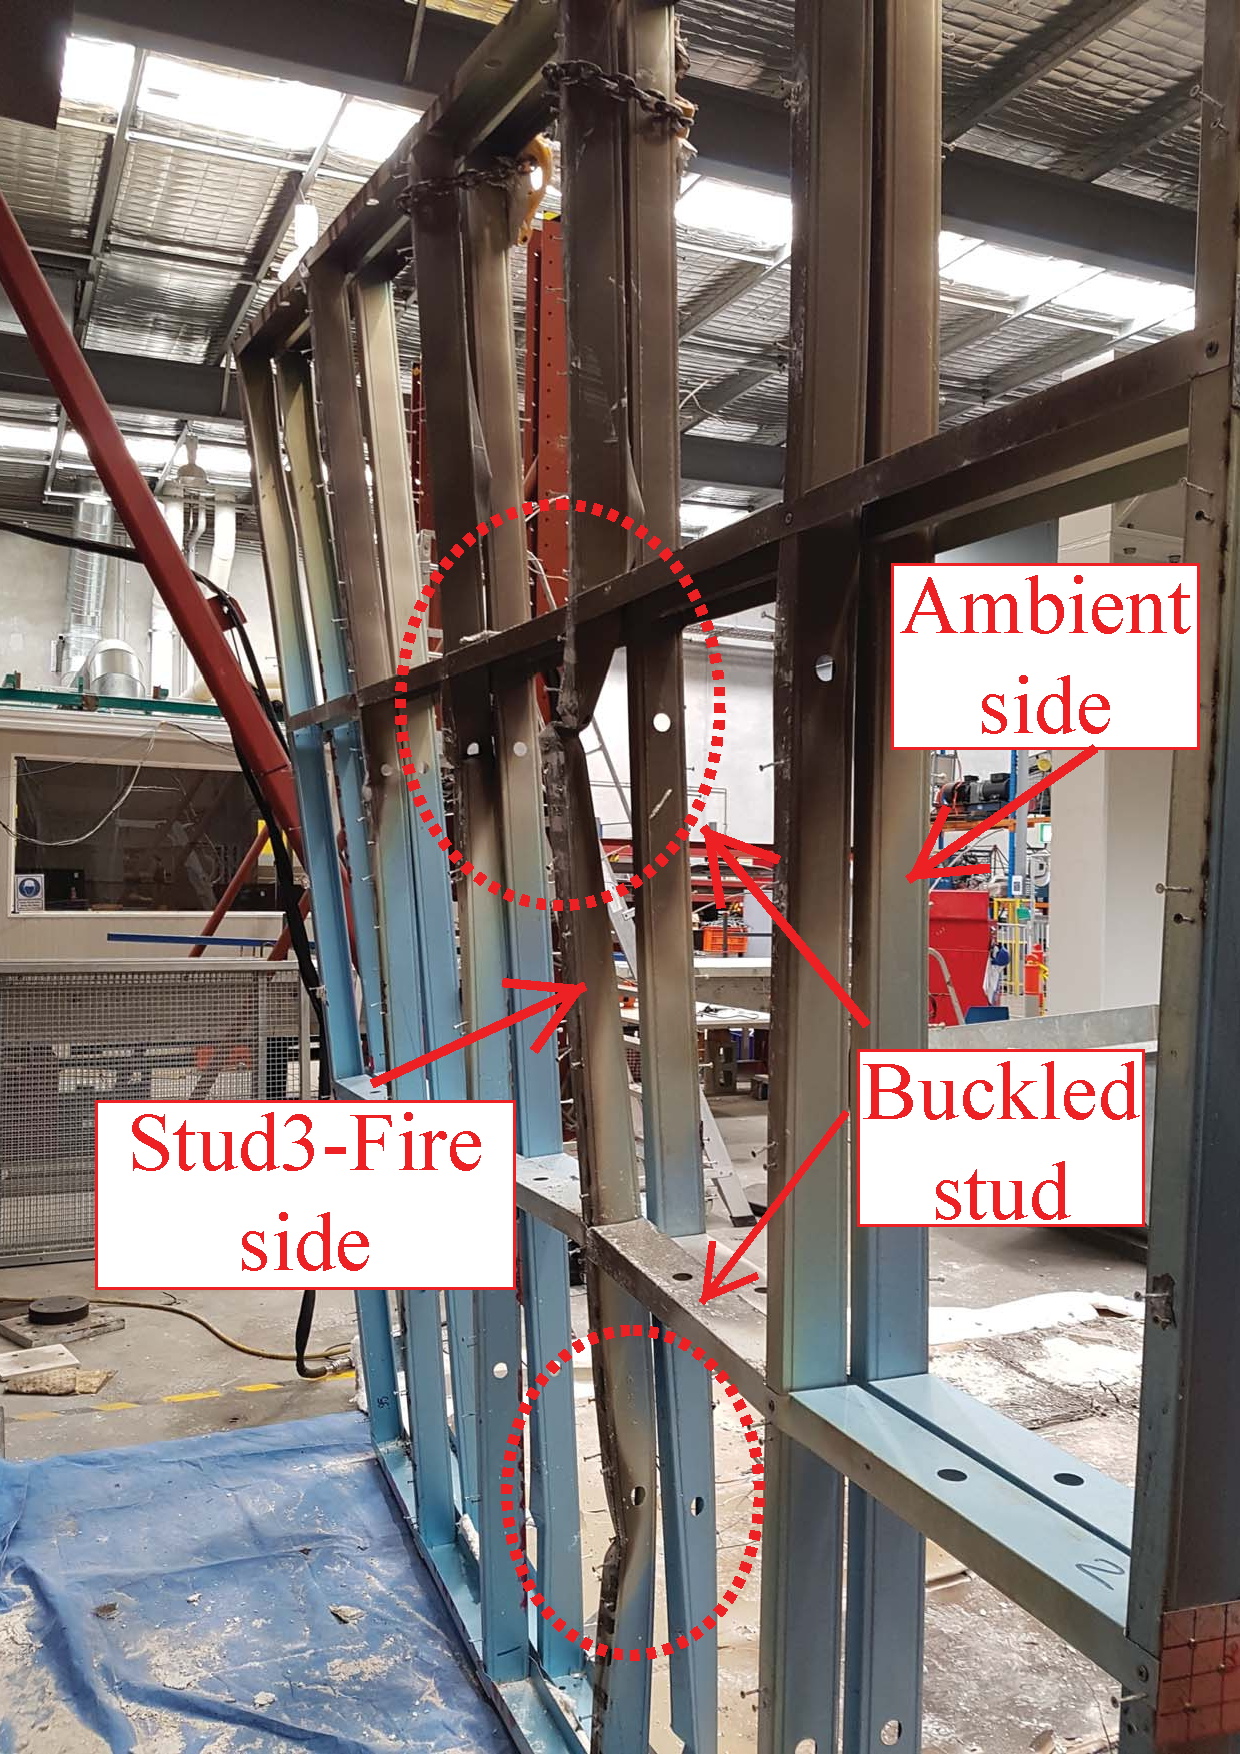
\includegraphics[scale=0.20]{T1-stud3-failure2.pdf} \\	 
			(a) & (b) & (c)  \\ 
		\end{tabular} 
		\caption{Failure of Test-T1 (a) Fire exposed side (b) Crack on ambient side plasterboard (c) Local compressive failure of Stud3}
		\label{fig:T1-failure}
\end{figure}

\subsection{Test-T1 Results and Discussion}

The time-temperature curves of the plasterboards and studs for Test-T1 are shown in \Cref{fig:T1-PB-Stud}. The fire exposed plasterboard temperature matched reasonably well with the standard fire curve. After 22 min of fire exposure, plasterboard joint compound started to fall-off indicating that the paper layer has been completely burnt. The Pb1 temperature at this stage was 740\degree C. No water droplets were visible till 40 min. At 41 min water patches were visible on the top right and left corners of the ambient side plasterboard. This was accompanied by mild smoke from the bottom of the test panel. There was visible smoke again at 75 min indicating the burning of paper layer. At this time the temperature recorded at Pb1-Pb2 was 638\degree C. The time-temperature curve on the fire side cavity (Pb2) was nearly flat during the early stages of the fire test until 60 min and the temperature recorded was well below 100\degree C as shown in \Cref{fig:T1-PB-Stud} (a). From 60 to 80 min the time-temperature curve suddenly increased with a steep slope to attain a peak value of 256\degree C and then increased gradually to a maximum value of 423\degree C at 176 min (at failure). It can also be noted that the steep rise is in correlation with the time-temperature curve recorded on the interface between the two plasterboard layers on the fire side (Pb1-Pb2). At 80 min the temperatures of fire side plasterboard (Pb1), the interface (Pb1-Pb2) and the fire side cavity (Pb2) were 963\degree C, 656\degree C and 256\degree C, respectively. The temperature difference between the fire side (Pb1) and the fire side interface (Pb1-Pb2) was 280\degree C whereas the difference between the interface (Pb1-Pb2) and fire side cavity (Pb2) was 400\degree C after 80 min of fire exposure. 
\begin{figure}[!htbp]
	\centering
		\begin{tabular}{cc}
			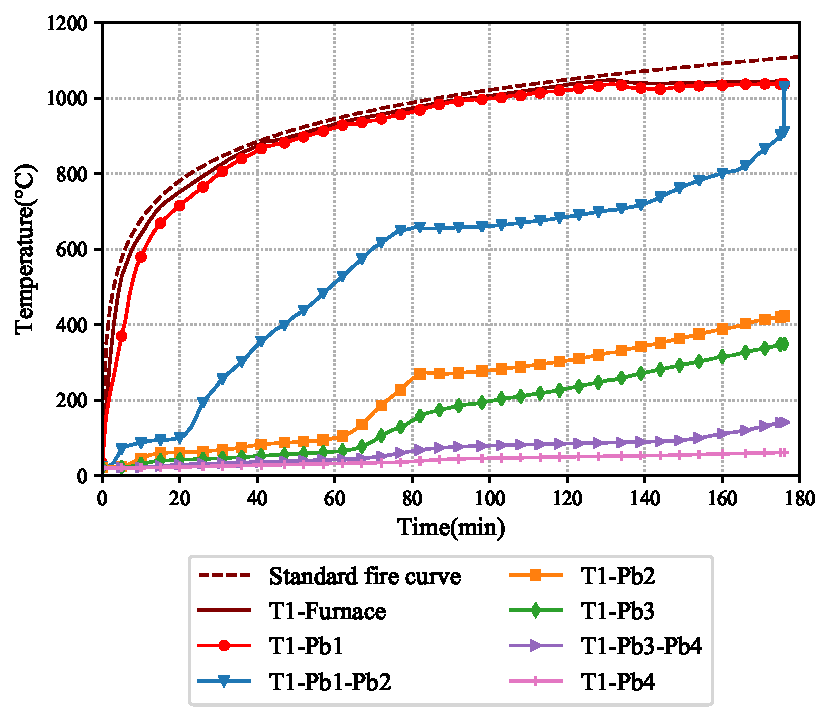
\includegraphics[width=7cm,height=6cm]{T1-Plasterboard} & 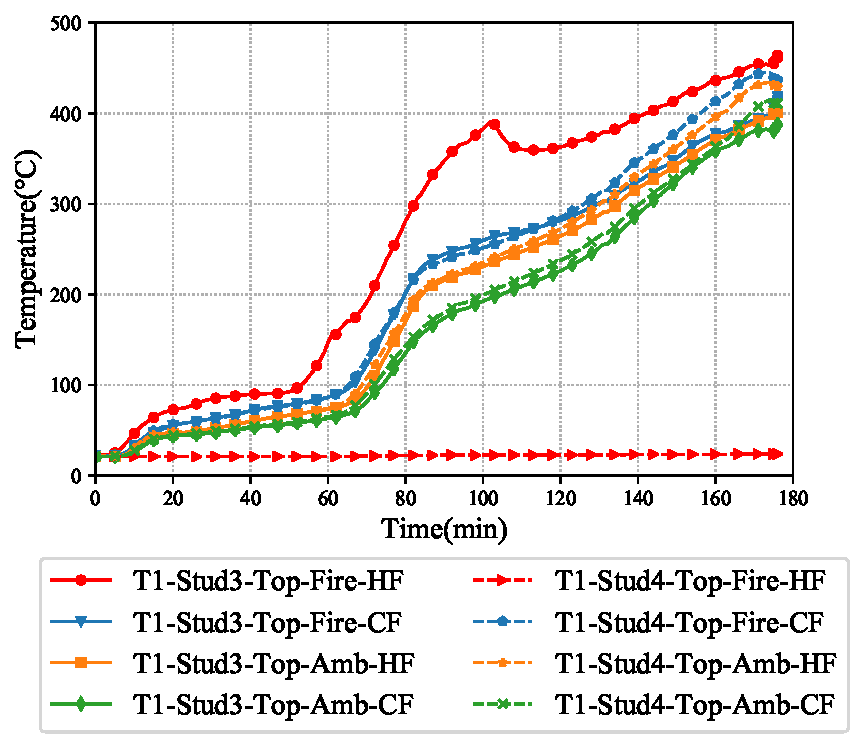
\includegraphics[width=7cm,height=6cm]{T1-Stud3-4-Top} \\ 
			(a) & (b)  \\ 
		\end{tabular} 
		\caption{Plasterboard and stud time-temperature curves of Test-T1 (a) Average plasterboard temperature (b) Stud3 temperature}
		\label{fig:T1-PB-Stud}
\end{figure}

Also during 80 to 120 min, the time-temperature curve of the Pb1- Pb2 interface as shown in \Cref{fig:T1-PB-Stud} (a) is nearly flat, whereas the time-temperature curve of Pb2 rises slowly. But the difference in temperature between these two surface is large. This infers that plasterboard has lost its ability to store heat at the interface (Pb1-Pb2). There is no significant rise in the time-temperature curve of Pb1-Pb2 during 80 to 120 min because the fire curve is also nearly flat during this time interval. The wider cavity in the double stud wall also has a significant contribution to this behaviour as the heat from Pb1-Pb2 surface gets transferred to Pb2, which emits it into the large cavity. The standard fire and Pb1 surface temperatures rise rapidly to 80 min but very slowly after 80 min. Therefore, the fire input to the wall is nearly constant helping the system to attain equilibrium during this time frame. Another important observation was that the time-temperature curve of Pb1-Pb2 increased suddenly from 20 to 80 min as shown in \Cref{fig:T1-PB-Stud} (a), which is in correlation with the standard fire curve.

The ambient side cavity (Pb3) time-temperature curve exhibited a similar behaviour to the fire side cavity (Pb2) curve. The first peak at 85 min was recorded as 166\degree C which is 90\degree C lower than the fire side cavity (Pb2) temperature of 256\degree C. The time-temperature curve of the ambient side interface (Pb3-Pb4) recorded a maximum temperature of 150\degree C at 176 min with the first peak of 67\degree C at 80 min. The curve then shows only a gradual rise which is in accordance with its source (Pb3). This indicates that cavity depth greatly influences the passage of heat from the fire exposed side to the ambient side because of natural convection within cavity. The ambient side plasterboard (Pb4) recorded a peak temperature of 68\degree C at 176 min, which is less than the limiting temperature of 180\degree C + room temperature at any point on the unexposed face or an average temperature of 140\degree C + room temperature on the unexposed face as specified in AS 1530.4 \citet{StandardsAustral2014}. This infers the absence of insulation failure in this fire test.

The time-temperature curves for Stud3 as recorded at the top (2250 mm) are shown in Fig.6 (b). They are used for discussion because of the severe local compressive failure observed at the top of Stud3 (\Cref{fig:T1-failure} (c)). The temperature curves showed no steep increase until 50 min of fire exposure.The hot flange temperatures on the fire and ambient sides were well below 100\degree C (T1-Stud3-Top-Fire-HF and T1-Stud3-Top-Amb-HF). From 50 to 80 min of fire exposure there was a sudden increase in the time-temperature curve on the fire side hot flange (T1-Stud3-Top-Fire-HF) reaching the first peak of 390\degree C at 102 min as shown in \Cref{fig:T1-PB-Stud} (b), followed by a small reduction in the temperature for about 10 min, reaching 358\degree C at 114 min. This reduction in temperature of 32\degree C is a result of the flat region in the temperature of plasterboards Pb1-Pb2 and Pb2, which act as a source for the fire side hot flange. From 120 min there was a gradual increase in the time-temperature curves of the fire side hot flanges until the end and recorded a temperature of 592\degree C at the end. The fire side cold flange (T1-Stud3-Top-Fire-CF) recorded 263\degree C at 102 min, which is 127\degree C less than the hot flange temperature . But the ambient side hot and cold flange temperatures at 102 min were 234\degree C (T1-Stud3- Top-Amb-HF) and 196\degree C (T1-Stud3-Top-Amb-CF), respectively. The difference in temperatures between the fire side hot and cold flanges was 127\degree C but the difference in temperature between the ambient side hot and cold flange was only 38\degree C. The difference in temperature between the fire side cold flange and ambient side hot flange was only 29\degree C.

The axial displacement and lateral deflection with respect to time are discussed in this section. The axial displacement was measured under the end plate that connected both rows of studs. The lateral deflection was measured at quarter heights (750 mm, 1500 mm, 2250 mm). In the fire tests the maximum deflection occurred at mid-height (1500 mm), which is considered in this discussion. In double stud LSF walls, LVDTs measured the lateral deflections only on ambient side studs. Therefore, it becomes difficult to predict the neutral axis shift as a result of thermal bowing in double stud LSF walls. The axial displacement and lateral deflection curves of the three fire tests are compared in Figs. \ref{fig:T1-Axial-Lateral} (a) and (b), respectively.
	\begin{figure}[!htbp]
	\centering
		\begin{tabular}{cc}
			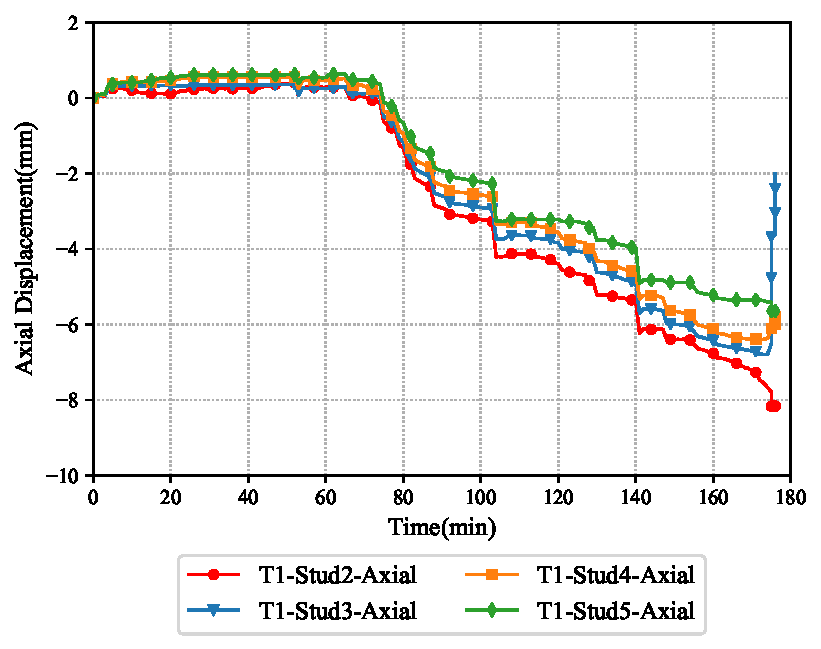
\includegraphics[width=7cm,height=6cm]{T1-Axial.pdf} & 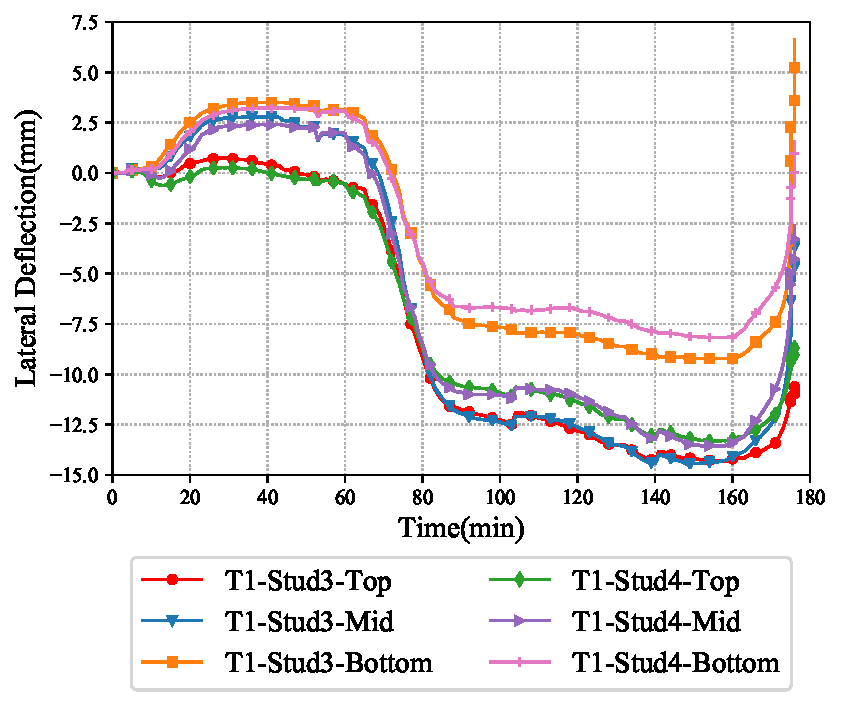
\includegraphics[width=7cm,height=6cm]{T1-Lateral.pdf} \\
			(a) & (b) \\
		\end{tabular} 
		\caption{Axial displacement and lateral deflection curves from Tests-T1 (a) Time vs Axial displacement (b) Time vs Lateral deflection curves}
		\label{fig:T1-Axial-Lateral}
\end{figure}

The axial displacement curve was almost flat for all the studs in fire till 60 min as shown in \Cref{fig:T1-Axial-Lateral} (a). This implies that no significant axial shortening occurred until 60 min of fire exposure. After this there was a steady increase in the axial displacement representing stud expansion due to fire exposure. This was observed till the end of fire test (176 min) after which the axial displacement curve changed sign and exhibited a sudden increase. The sudden increase in the curve is due to the axial contraction of the studs indicating structural failure of the test wall. The lateral deflection curve with respect to time recorded at mid-height (1500 mm) is shown in \Cref{fig:T1-Axial-Lateral} (b). The curve was nearly flat until 75 min. There was a small inward bowing of studs measuring 2 mm until 75 min after which the lateral deletion curve dropped to -11.16 mm at 82 min and reached a maximum of -14.44 mm in Stud3 (T1-Stud3-Mid) at the end of the test. This indicates that there was an outward thermal bowing on the ambient side studs. It is to be noted that the lateral deflection is for the ambient side studs only.

\section{Fire Test-T2}

This test was conducted with 0.75 mm thick studs to determine the fire performance of double stud walls with thinner stud sections. Ambient capacity test conducted on the wall initially gave a stud capacity of 45.87 kN. Each stud was subjected to an axial compression load of 18.34 kN to simulate the same load ratio of 0.4 as in Test-T1. The test wall panel failed after 132 min due to structural inadequacy. Unlike Test-T1, there was a significant plasterboard fall-off on the fire exposed side (Pb1) as shown in \Cref{fig:T2-failure} (a). However, no cracks were observed on the ambient side of plasterboard. Discolouration of plasterboard was observed on the ambient side top right corners at the end of fire test (\Cref{fig:T2-failure} (b)). Studs 4 and 5 were subjected to severe local compressive failures as shown in \Cref{fig:T2-failure} (c).

\begin{figure}[!htbp]
	\centering
		\begin{tabular}{ccc}
			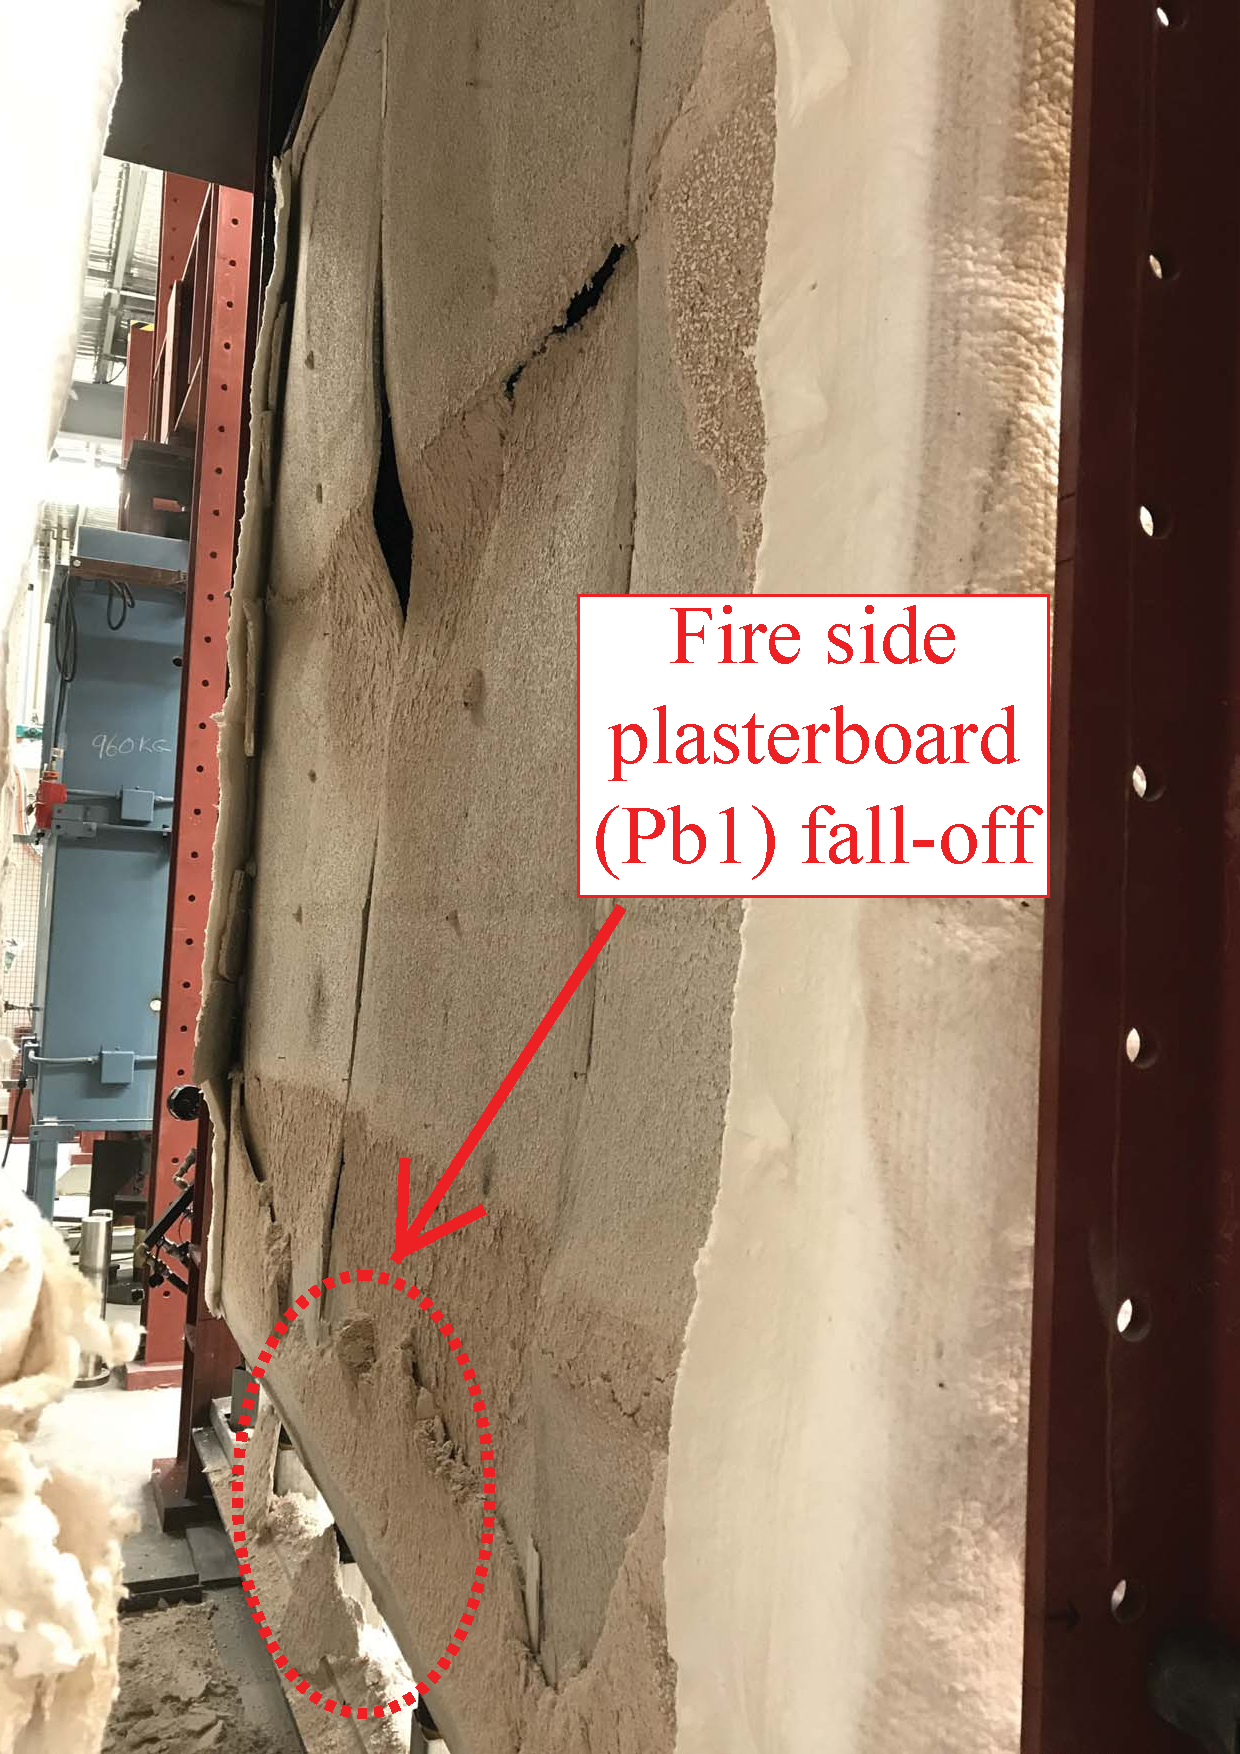
\includegraphics[scale=0.20]{T2-fire-side2.pdf} & 
			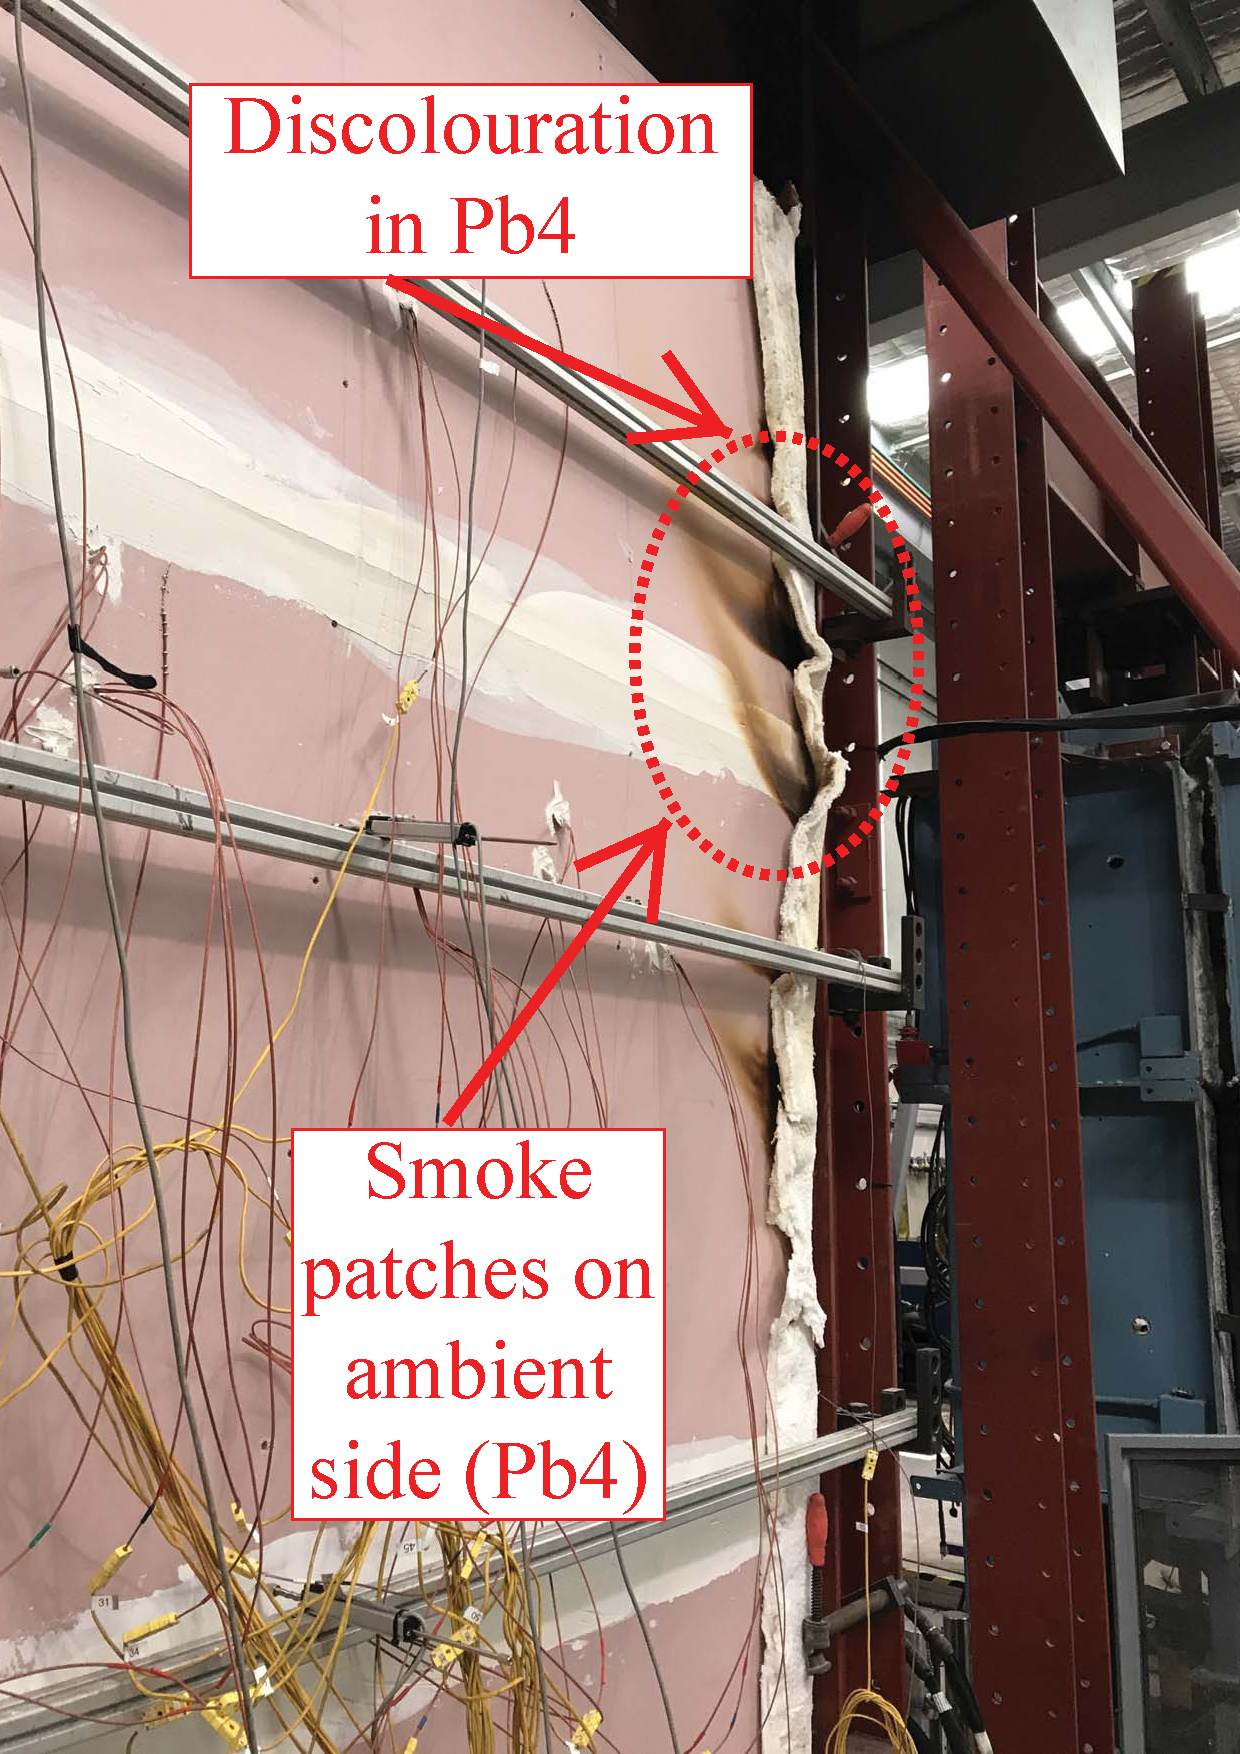
\includegraphics[scale=0.20]{T2-ambient-side2.pdf} &
			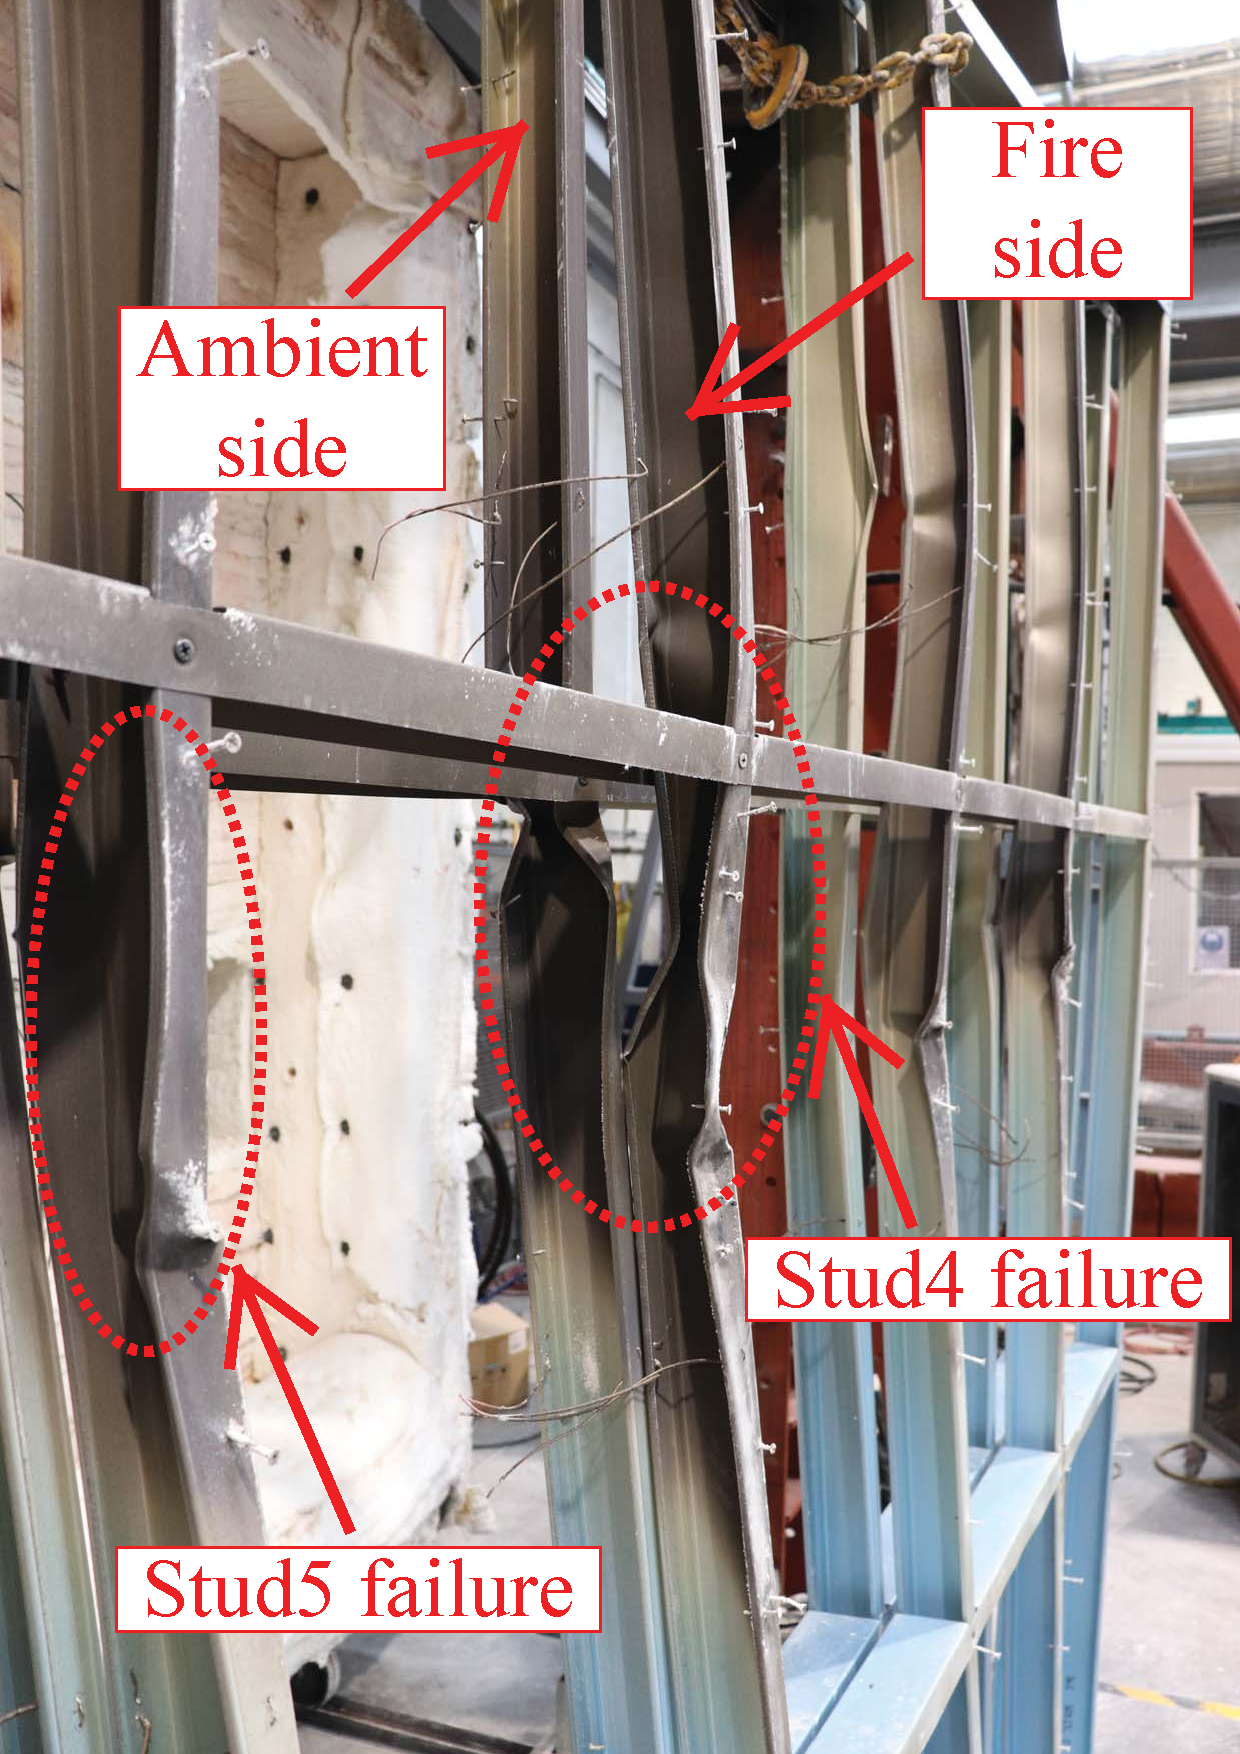
\includegraphics[scale=0.20]{T2-stud4-failure2.pdf} \\	 
			(a) & (b) & (c)  \\ 
		\end{tabular} 
		\caption{Failure of Test-T2 Panel (a) Fire exposed side (b) Smoke patches on ambient side plasterboard (c) Local compressive failure of Stud4}
		\label{fig:T2-failure}
\end{figure}

\subsection{Test-T2 Results and Discussion}

The standard fire curve was achieved with good agreement. The time- temperature curve of Pb1-Pb2 interface was similar to Test-T1 till 25 min of fire exposure. Water droplets were visible near the bottom after 30 min. Similar to Test-T1 the time-temperature curve of Pb1-Pb2 interface showed a steep rise and reached a maximum of 709\degree C at 84 min. This was followed by a flat region until 110 min. Unlike Test-T1 this flat region did not last for a longer period of time. This is because of the fire side plasterboard fall-off as shown in \Cref{fig:T2-failure} (a). Such plasterboard fall-off on the fire side makes a significant contribution to the difference in the time-temperature curve between the two tests T1 and T2. The corresponding temperature on the fire side plasterboard (Pb1) was 971\degree C at 82 min, which acts as a source for Pb1-Pb2 interface.

The time-temperature curve on the fire side cavity (Pb2) also exhibited a similar behaviour as for Test-T1. The temperature was well below 100\degree C for the initial 60 min. There was a sudden increase in the curve from 60 to 80 min and attained the first peak of 342\degree C at 82 min. Then the curve was nearly flat and showed only a gradual increase till the end. The maximum temperature recorded at the end of fire test (132 min) was 443\degree C. The difference in temperature at 82 min between Pb1-Pb2 and Pb2 was 348\degree C. The ambient side cavity Pb3 was nearly flat until 75 min as shown in \Cref{fig:T2-PB-Stud} (a). The temperature difference between Pb2 and Pb3 at 82 min was 170\degree C. After 82 min there was a gradual increase in the time-temperature curve reaching a maximum of 395\degree C at the end. Time-temperature curves of the ambient side plasterboard interface Pb3-Pb4 and ambient side Pb4 recorded a maximum of 128\degree C and 58\degree C at the end (132 min). The ambient side plasterboard temperatures did not exceed the average and the maximum insulation temperature limits \citet{StandardsAustral2014}, indicating no insulation failure in fire test.

\begin{figure}[!htbp]
	\centering
		\begin{tabular}{cc}
			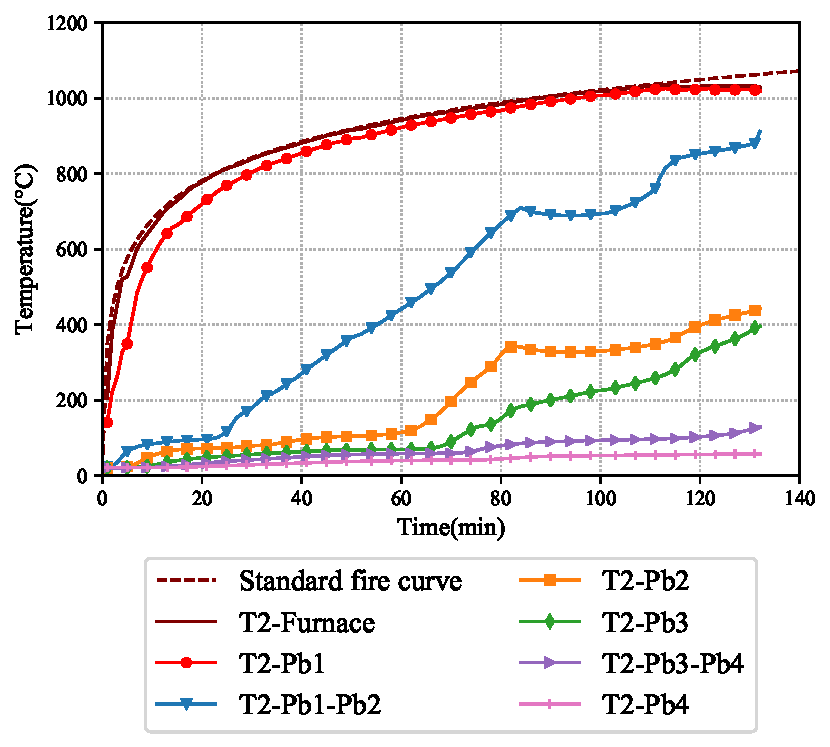
\includegraphics[width=7cm,height=6cm]{T2-Plasterboard} & 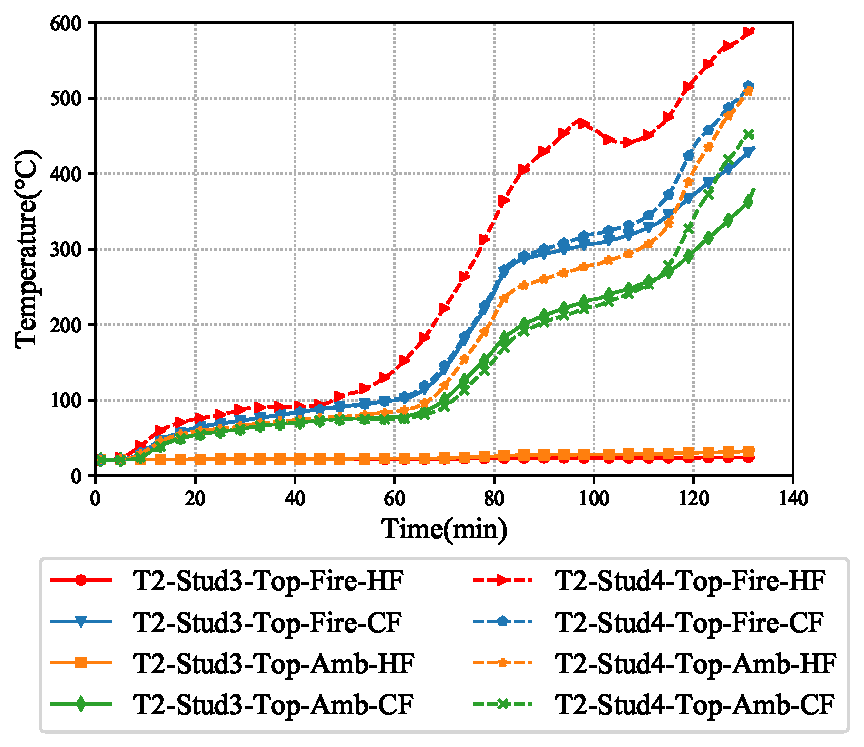
\includegraphics[width=7cm,height=6cm]{T2-Stud3-4-Top} \\ 
			(a) & (b)  \\ 
		\end{tabular} 
		\caption{Plasterboard and stud time-temperature curves of Test-T2 (a) Average plasterboard temperatures (b) Stud4 temperatures}
		\label{fig:T2-PB-Stud}
\end{figure}

The time-temperature curves of Stud4 recorded at the top of Stud4 (2250 mm) are shown in \Cref{fig:T2-PB-Stud} (b) as the local compressive failure was severe at the top of Stud4 as shown in \Cref{fig:T2-failure} (c). Temperatures recorded at the top of the stud were found to be higher at the top of Stud4 in comparison with other studs. The time-temperature curve on the fire side hot flange (T2-Stud4-Top-Fire-HF) was nearly flat till 55 min and the temperatures recorded were well below 100\degree C. From 55 min the curve exhibited a steep rise reaching the first peak of 470\degree C at 97 min. There was a reduction in temperature at 106 min measuring 441\degree C as shown in \Cref{fig:T2-PB-Stud} (b). The difference in temperature during this 9 min time period was 29\degree C. This behaviour was similar to that of the fire side hot flange time-temperature curve observed in Test-T1. The curve started to rise rapidly from 110 min and recorded a temperature of 592\degree C at the end. The time-temperature curve of the fire side cold flange (T2-Stud4-Top-Fire- CF) followed a trend similar to the fire side hot flange till 60 min. There was a steep increase in the time-temperature curve from 60 to 80 min after which the rise was gradual until 110 min. The ambient side hot and cold flanges exhibited a behaviour similar to the fire side cold flange. The corresponding temperatures of the fire side cold flange (T2-Stud4-Top-Fire-CF), the ambient side hot flange (T2-Stud4-Top-Amb-HF) and the ambient side cold flange (T2-Stud4-Top-Amb-CF) were 451\degree C, 344\degree C, 307\degree C and 253\degree C, respectively. The difference between the fire side hot and cold flanges was 107\degree C while the difference between the ambient side hot and cold flange was 54\degree C. But the difference between the fire side cold flange and ambient side hot flange was only 37 \degree C . The peak temperatures of the fire side hot flange (T2-Stud4-Top-Fire-HF), fire side cold flange (T2-Stud4-Top-Fire-CF), the ambient side hot flange (T2-Stud4-Top-Amb-HF) and the ambient side cold flange (T2-Stud4-Top-Amb-CF) were 592\degree C, 516\degree C, 508\degree C and 451\degree C at the end of the fire test.

The axial displacement and lateral deflection with respect to time corresponding to Test-T2 are presented in \Cref{fig:T2-Axial-Lateral}. The axial displacement was measured in a similar way similar to Test-T1. LVDT T2-Stud4-Axial malfunctioned and should be ignored.
	\begin{figure}[!htbp]
	\centering
		\begin{tabular}{cc}
			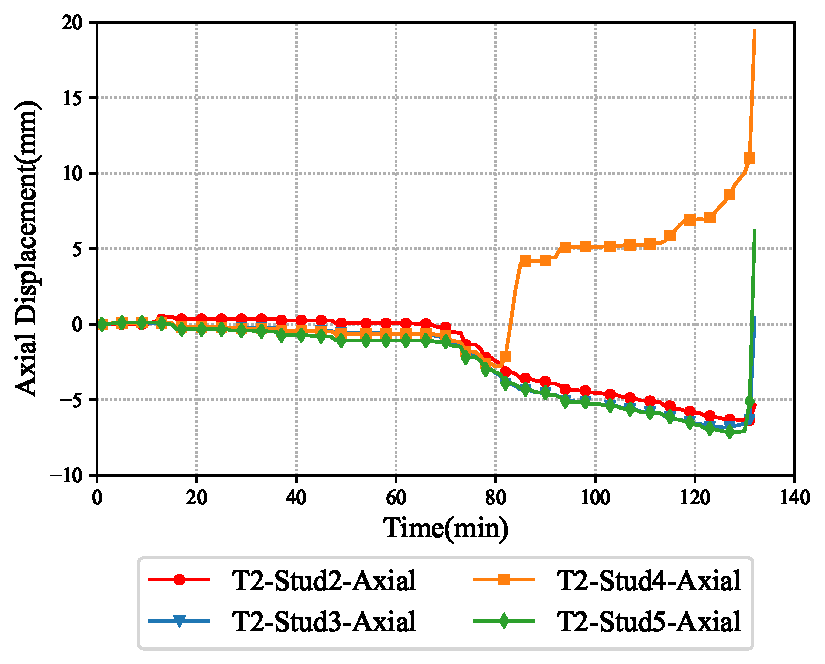
\includegraphics[width=7cm,height=6cm]{T2-Axial.pdf} & 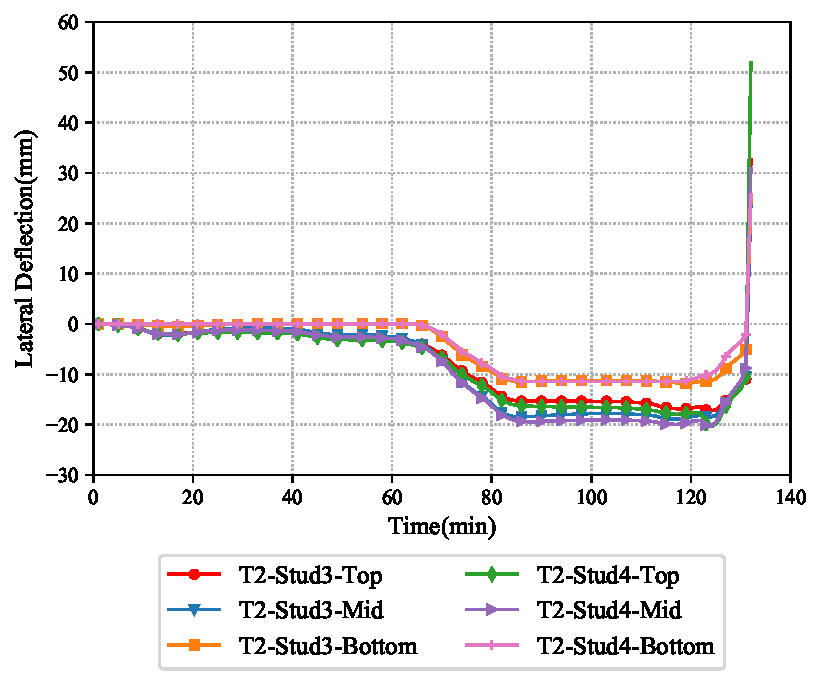
\includegraphics[width=7cm,height=6cm]{T2-Lateral.pdf} \\
			(a) & (b) \\
		\end{tabular} 
		\caption{Axial displacement and lateral deflection curves from Tests-T2 (a) Time vs Axial displacement (b) Time vs Lateral deflection curves}
		\label{fig:T2-Axial-Lateral}
\end{figure}

In Test-T2 there were small axial displacement measuring 1.083 mm in T2-Stud5-Axial at 60 min. The maximum axial displacement was 7.13 mm in T2-Stud5-Axial at 132 min. The axial displacement in Test-T1 is less than in Tests-T2 and T3 due to the use of thinner studs in the later. The lateral deflection exhibited outward thermal bowing from the start of the fire test. A maximum lateral deflection of -20.25 mm was recorded in Stud4 (T2-Stud4-Mid). 

\section{Fire Test-T3}

Test-T3 was conducted to investigate the fire performance of double stud LSF walls made of 0.75 mm thick LCS studs under a higher LR of 0.6 (28.25 kN per stud). The wall panel failed after 81 min due to structural inadequacy in Stud3 as shown in \Cref{fig:T3-failure} (c). Plasterboard fall-off was noticed in a small region on the fire side (Pb1) after the fire test as shown in \Cref{fig:T3-failure} (a) while the ambient side plasterboard had no cracks or smoke patches. Water droplets were visible on the bottom of the wall due to dehydration process after 32 min.
\begin{figure}[!htbp]
	\centering
		\begin{tabular}{ccc}
			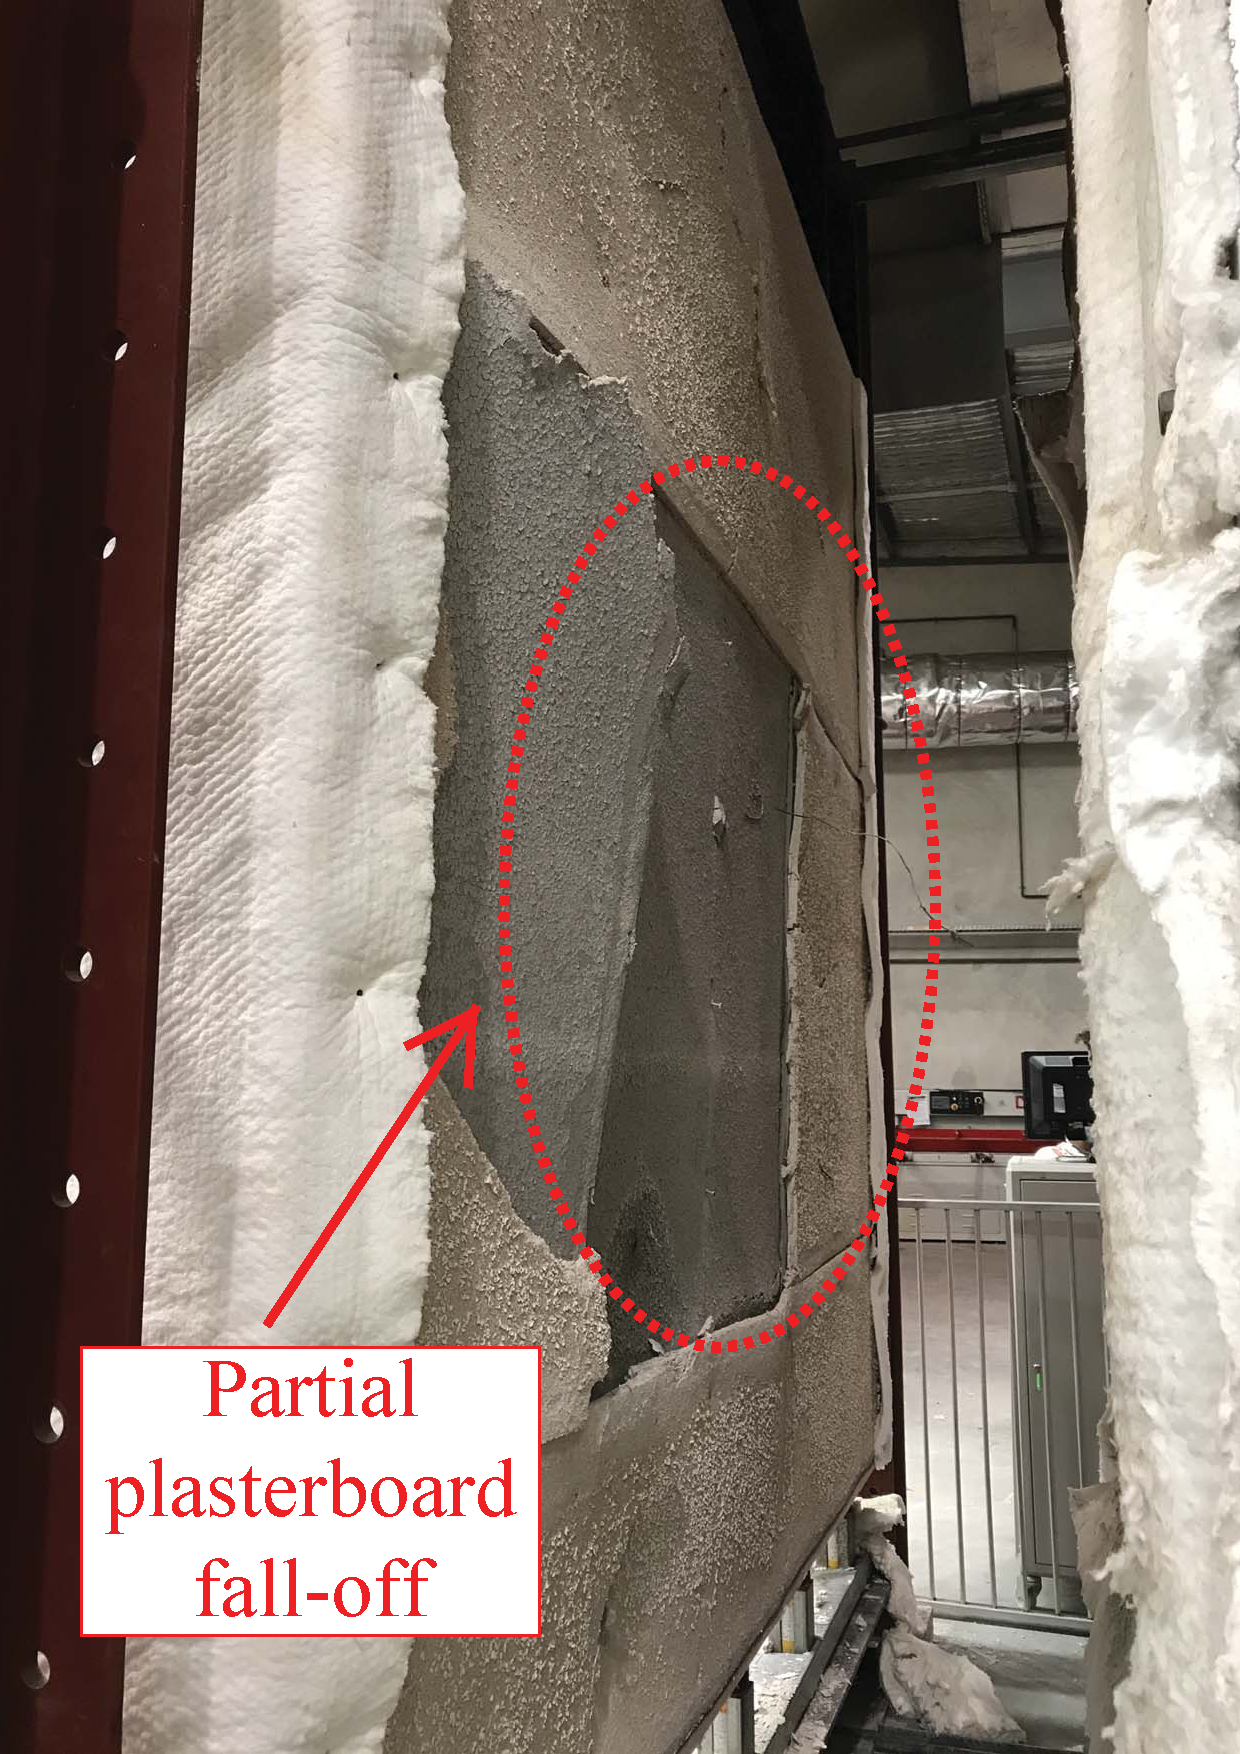
\includegraphics[scale=0.20]{T3-fire-side2.pdf} & 
			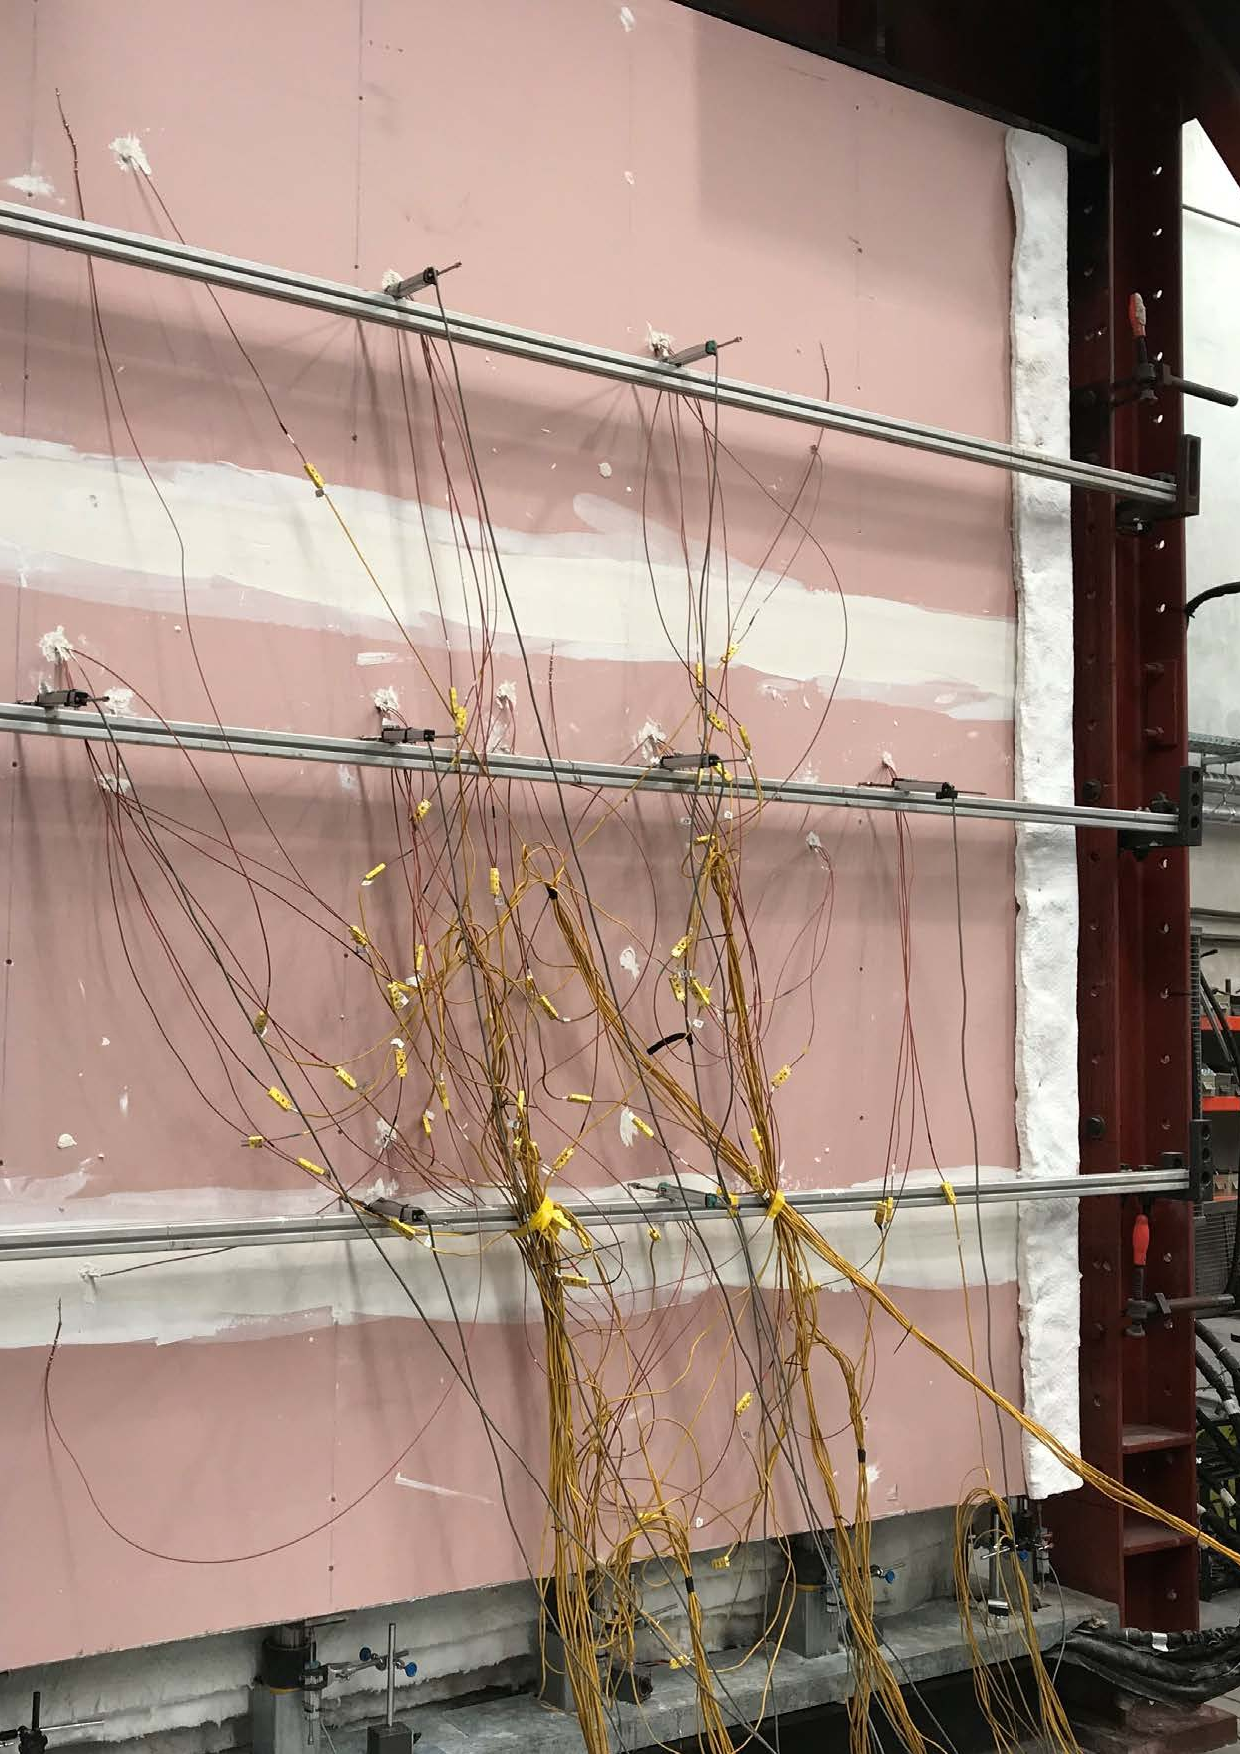
\includegraphics[scale=0.20]{T3-ambient-side2.pdf} &
			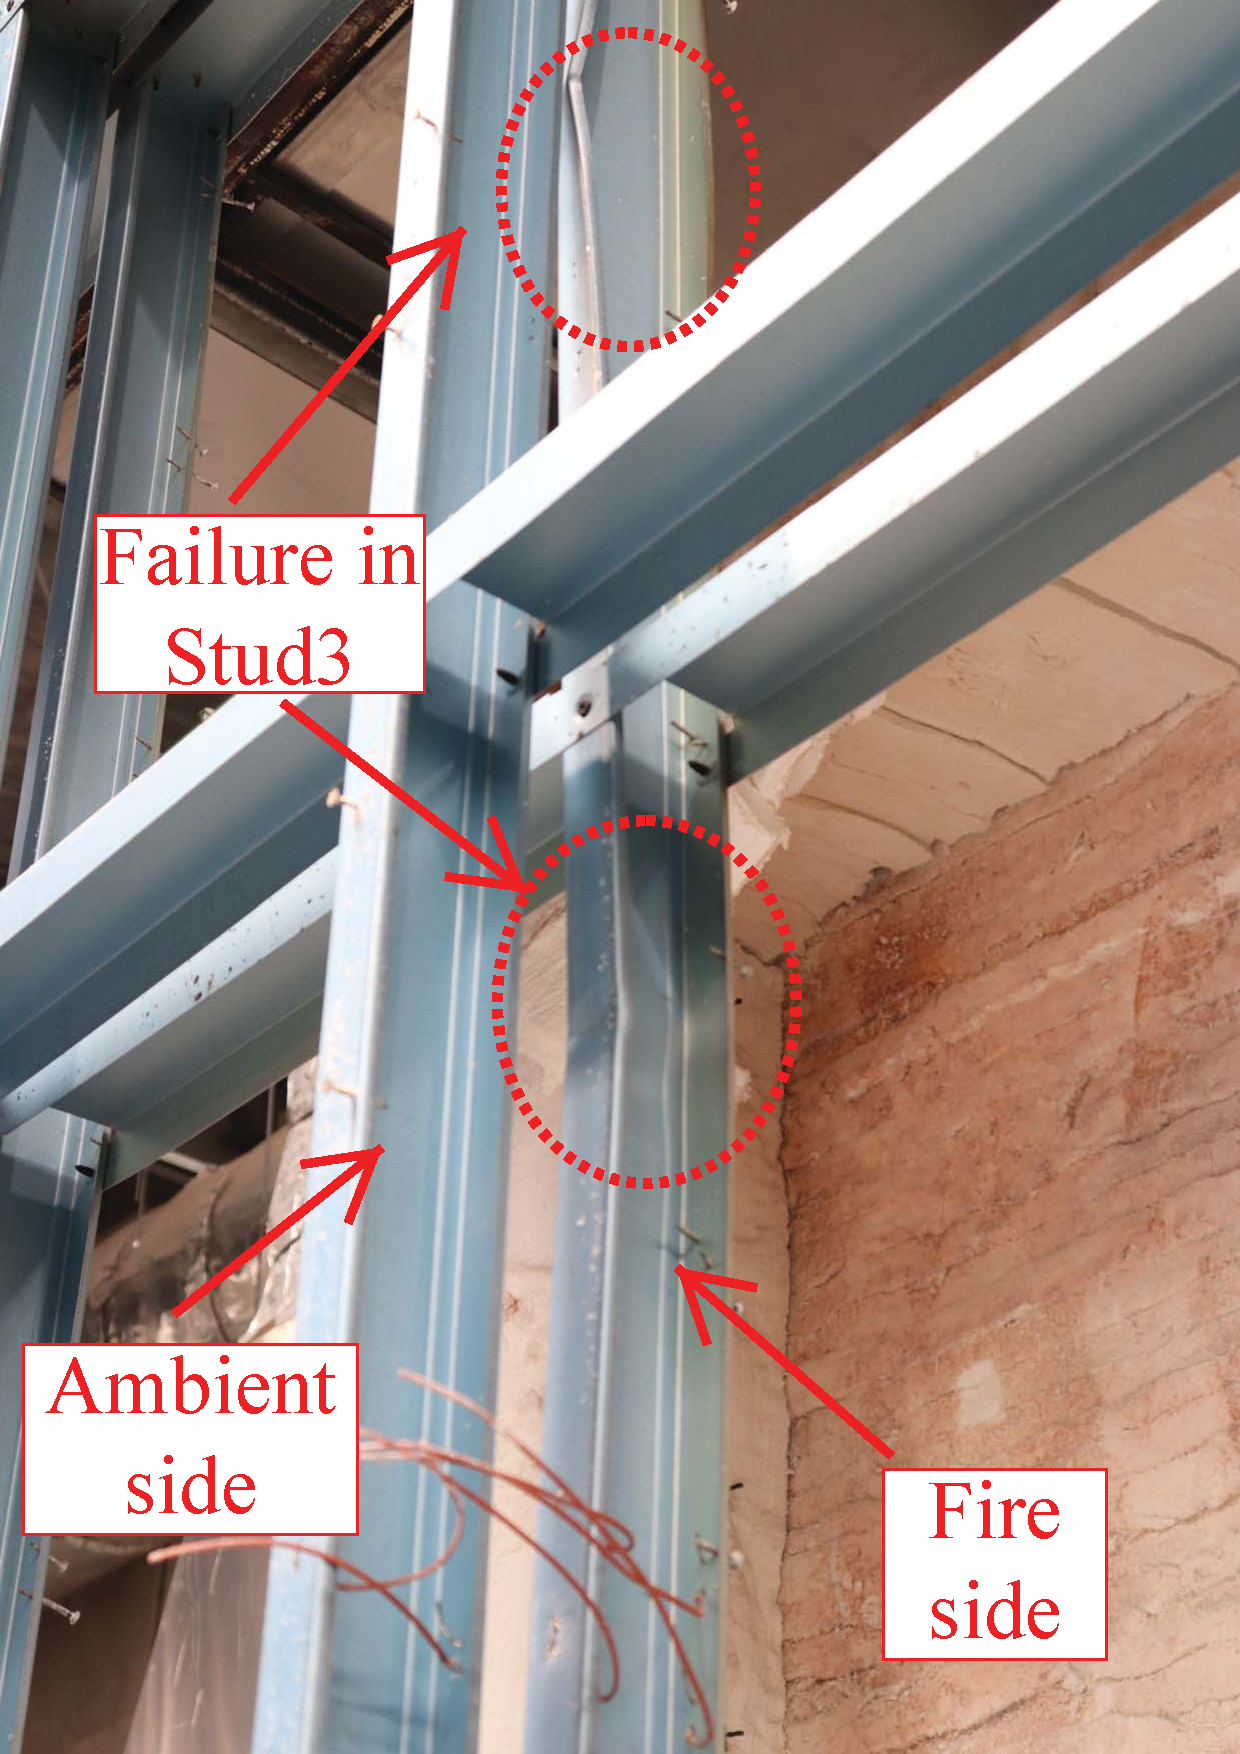
\includegraphics[scale=0.20]{T3-stud4-failure2.pdf} \\	 
			(a) & (b) & (c)  \\ 
		\end{tabular} 
		\caption{Failure of Test-T3 Panel (a) Fire exposed side (b) Ambient side plasterboard (c) Local compressive failure of Stud3}
		\label{fig:T3-failure}
\end{figure}

\subsection{Test-T3 Results and Discussion}

The time-temperature curve on the fire side (Pb1) matched reasonably well with the standard fire curve. The Pb1-Pb2 interface curve was flat until 25 min with temperatures less than 100\degree C. From 25 to 80 min, it rose rapidly, reaching a maximum of 651\degree C at 81 min as shown in \Cref{fig:T3-PB-Stud} (a). This test does not exhibit the unique behaviour of the time-temperature curve remaining flat from 80 min as observed in Tests-T1 and T2. This is because the fire test lasted only 81 min under the higher LR. The Pb1-Pb2 temperature dropped slightly to 633\degree C at 81 min. This 18\degree C difference in temperature happened within a short period of 2 min. This is where the phase change happens in the cavity similar to Test-T2. But due to the sudden plasterboard fall-off and the higher load ratio the test panel could not survive any further.
	\begin{figure}[!htbp]
		\centering
			\begin{tabular}{cc}
				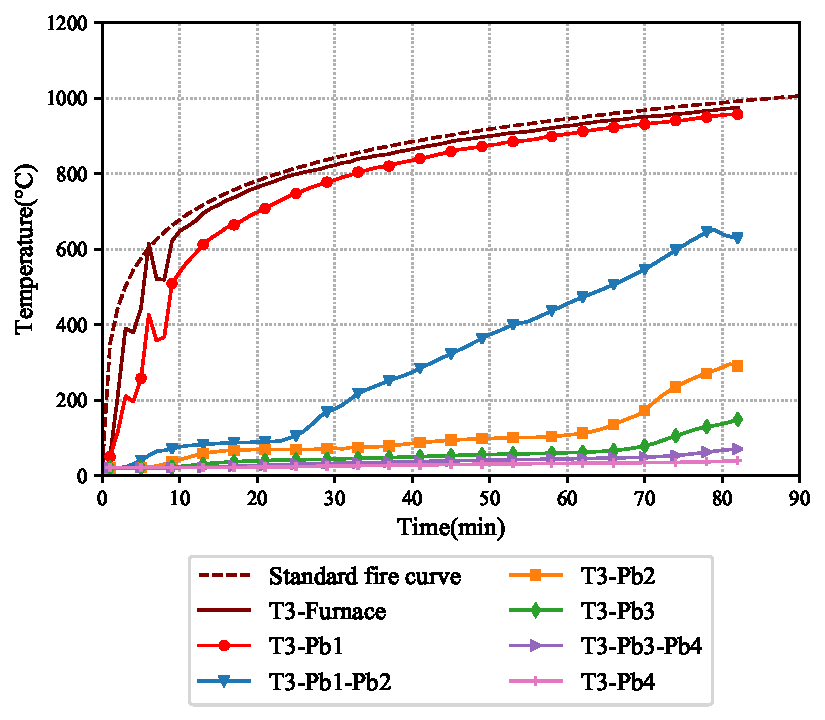
\includegraphics[width=7cm,height=6cm]{T3-Plasterboard.pdf} & 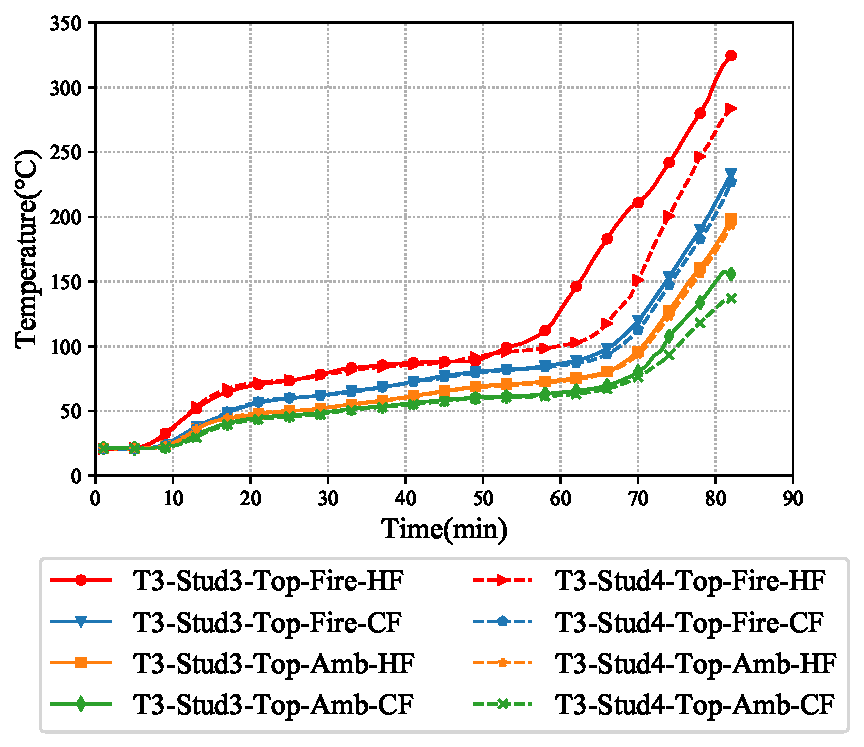
\includegraphics[width=7cm,height=6cm]{T3-Stud3-4-Top.pdf} \\ 
				(a) & (b)  \\ 
			\end{tabular} 
			\caption{Plasterboard and stud time-temperature curves of Test-T3 (a) Average plasterboard temperatures (b) Stud3 temperatures}
			\label{fig:T3-PB-Stud}
	\end{figure}

The time-temperature curve on the fire side cavity (Pb2) was below 100\degree C till 52 min with a sudden increase during 65 to 80 min to reach a peak temperature of 295\degree C at 81 min (end of fire test). Plasterboard on the ambient side cavity recorded temperatures less than 100\degree C until 75 min after which there was a gradual rise reaching a maximum of 149\degree C at the end. The temperatures on the ambient side plasterboard interface (Pb3-Pb4) and ambient side (Pb4) recorded 71\degree C and 39\degree C, respectively, indicating no insulation failure as per AS 1530.4 \citet{StandardsAustral2014}.

The time-temperature curves of the studs also did not exhibit the drop in the fire side hot flange temperatures as seen in Tests-T1 and T2. Local compressive failure was observed at the top of Stud3 as shown in \Cref{fig:T3-failure} (c) and hence the time-temperature curves recorded at the top of Stud3 (\Cref{fig:T3-PB-Stud} (b) are used here for discussion. The fire side hot flange temperature (T3-Stud3-Top-Fire-HF) was below 100\degree C until 55 min with a steep rise to reach a maximum temperature of 332\degree C at the end of the test. The fire side cold flange (T3-Stud3-Top-Fire-CF) recorded a temperature less than 100\degree C until 65 min after which there was a steep rise, reaching the maximum temperature of 226\degree C at the end, which is 106\degree C less than the corresponding hot flange. The ambient side hot and cold flanges followed a similar trend to that of fire side cold flange. The maximum temperatures recorded at T3-Stud3-Top-Amb-HF and T3-Stud3-Top-Amb-CF were 187\degree C and 157\degree C, respectively, with 30\degree C difference. The difference in temperature between the fire side cold flange and ambient side hot flange temperature was 39\degree C at the end of the fire test.

The axial displacement and lateral deflection with respect to time are discussed in this section. The axial displacement was measured under the end plate that connected both rows of studs. The lateral deflection was measured at quarter heights (750 mm, 1500 mm, 2250 mm). In the fire tests the maximum deflection occurred at mid-height (1500 mm), which is considered in this discussion. In double stud LSF walls, LVDTs measured the lateral deflections only on ambient side studs. Therefore, it becomes difficult to predict the neutral axis shift as a result of thermal bowing in double stud LSF walls. The axial displacement and lateral deflection curves of the three fire tests are compared in \Cref{fig:T1-Axial-Lateral} (a) and (b), respectively. LVDT T2-Stud4-Axial malfunctioned and should be ignored.
\begin{figure}[!htbp]
	\centering
		\begin{tabular}{cc}
			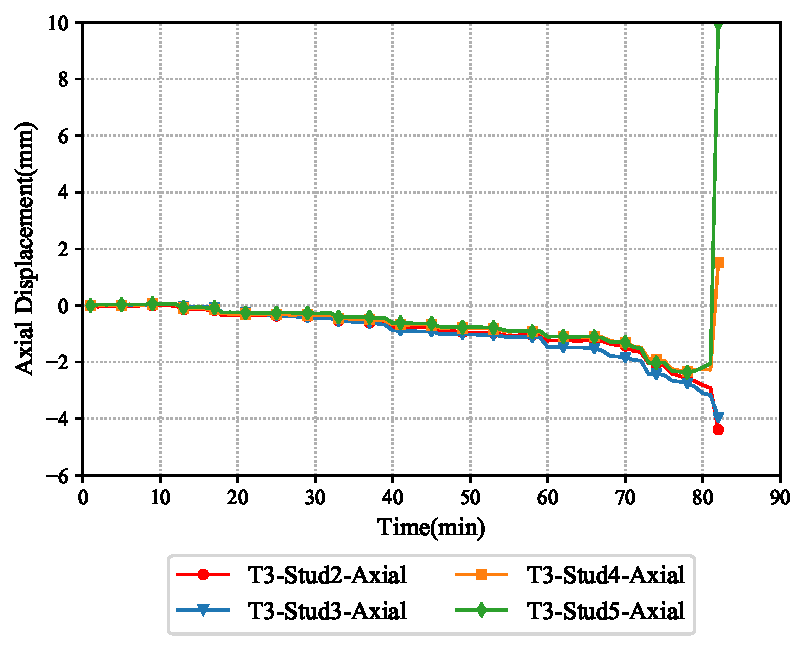
\includegraphics[width=7cm,height=6cm]{T3-Axial} & 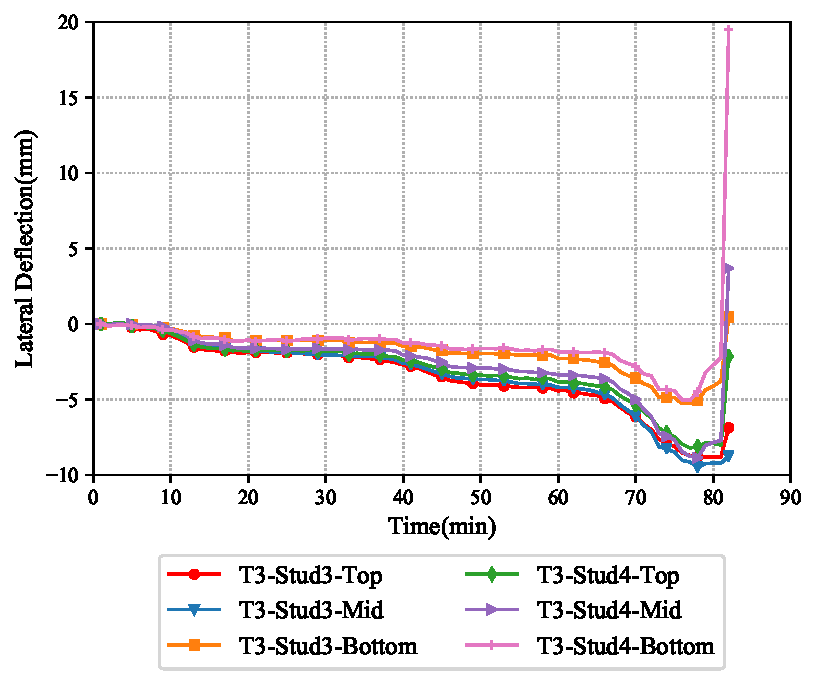
\includegraphics[width=7cm,height=6cm]{T3-Lateral} \\
			(a) & (b) \\
		\end{tabular} 
		\caption{Axial displacement and lateral deflection curves from Tests-T3 (a) Time vs Axial displacement (b) Time vs Lateral deflection curves}
		\label{fig:T3-Axial-Lateral}
\end{figure}

The axial displacement curve was almost flat for all the studs in fire Test-T1 till 60 min as shown in \Cref{fig:T3-Axial-Lateral} (a). But in Tests-T2 and T3 there were small displacements measuring 1.083 mm in T2-Stud5-Axial and 1.47 mm in T3-Stud3-Axial at 60 min. This implies that no significant axial shortening occurred until 60 min of fire exposure in all three fire tests. Test-T1 curve showed a gradual increase in the axial displacement reaching a maximum of 8.17 mm in T1-Stud2- Axial. But in Tests-T2 and T3 the curve was steep. For Test-T2 the maximum axial displacement was 7.13 mm in T2-Stud5-Axial at 132 min. Likewise for Test-T3 the maximum axial displacement was 3.95 mm in T3-Stud3-Axial at 81 min. The corresponding deflections at 81 min in Tests-T1 and T2 were 1.68 mm and 3.41 mm. The axial displacement in Test-T1 is less than in Tests-T2 and T3 due to the use of thinner studs in the later.

The lateral deflection curve with respect to time recorded at mid-height (1500 mm) is shown in \Cref{fig:T3-Axial-Lateral} (b). For Test-T1 the curve was nearly flat until 75 min. There was a small inward bowing of studs measuring 2 mm until 75 min after which the lateral deletion curve dropped to -11.16 mm at 82 min and reached a maximum of -14.44 mm in Stud3 (T1-Stud3-Mid) at the end of the test. This indicates that there was an outward thermal bowing on the ambient side studs. It is to be noted that the lateral deflection is for the ambient side studs only. The lateral deflection in Tests-T2 and T3 exhibited outward thermal bowing from the start of the fire test. Test-T2 exhibited a maximum lateral deflection of -20.25 mm in Stud4 (T2-Stud4-Mid) while Test-T3 recorded a maximum outward deflection of -9.43 mm in Stud3 (T3-Stud3-Mid). The lateral deflections recorded in Tests-T2 and T3 were higher than Test-T1 deflection. This is also because of the use of thinner studs used in Tests-T2 and T3.

\section{Fire Test-T4}

To determine the fire performance of double stud wall with a reduced cavity depth Test-T4 was conducted with 70 mm wide studs. Along with a 20 mm air gap between the two rows of stud, the effective cavity depth maintained in this test wall was 160 mm. Plan view of Test-T4 is shown in \Cref{fig:T4-plan} below. Initial ambient capacity test resulted in a maximum axial compression capacity of 86.21 kN and an LR of 0.4 (34.48 kN) was used to conduct the full-scale fire test.      
\begin{figure}[!htbp]
	\centering
	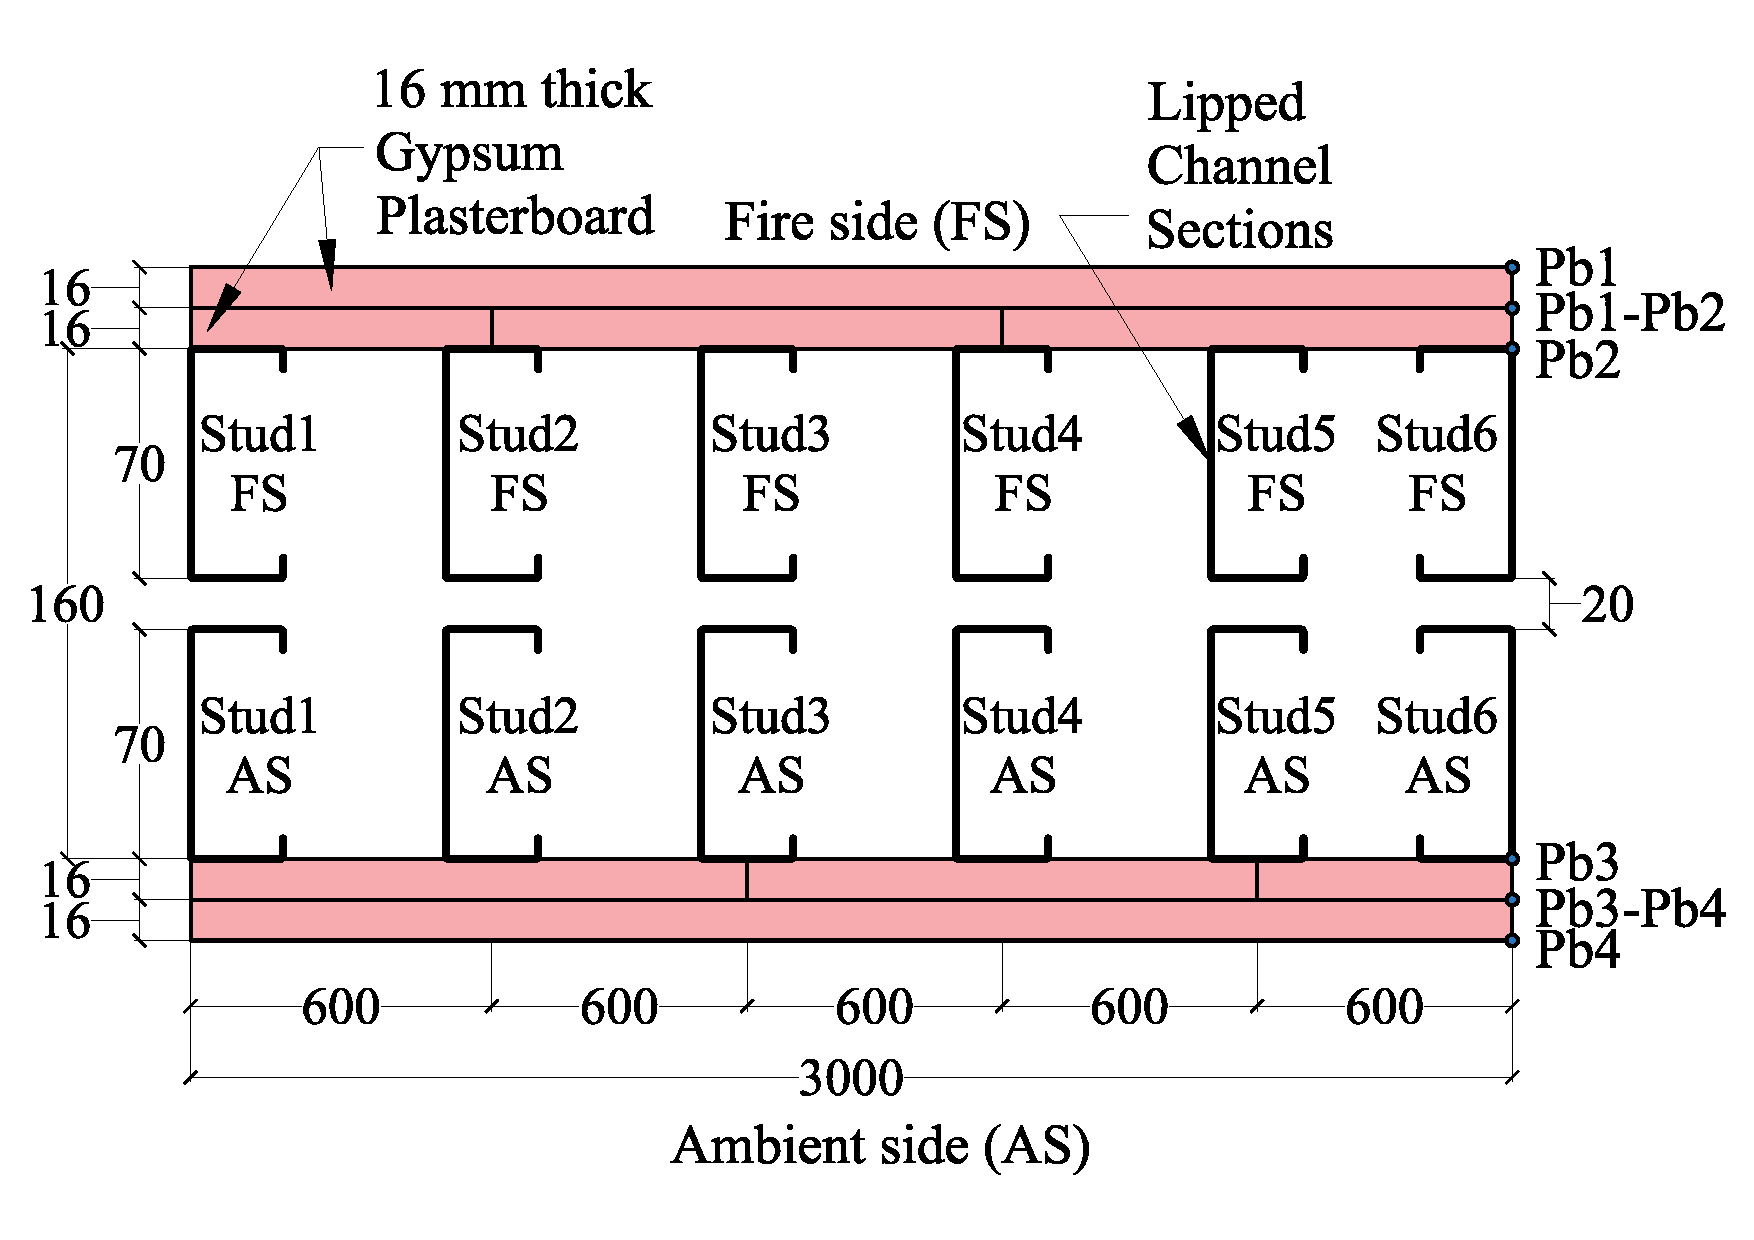
\includegraphics[width=9cm, height=5cm]{T4-plan.pdf}
	\caption{Plan view of Double Stud LSF Wall Panel}
	\label{fig:T4-plan}
	\fontsize{10}{1}\textit{Note : All dimensions are in mm.}
\end{figure}

After 17 min from the start of the fire test a cracking sound was heard. This was followed by joint compound fall-off at 30 min. A small patch of smoke was visible from the top left corner of the test specimen at 34 min indicating calcination of the fire side plasterboard. At 86 of the fire test, smoke was visible from the top right corner of the test specimen. This indicates the calcination of the second layer of plasterboard on the fire side. A crack on the fire side plasterboard was noticeable through furnace camera at 120 min which resulted in a small portion of the fire side plasterboard to fall-off at 132 min. The fall-off was witnessed near the plasterboard joints which are prone to be the weakest part of the test specimen in a full-scale fire test. The test specimen survived for 171 min after which the test wall could not withstand the applied axial load experiencing a drop load indicating failure due to structural inadequacy.

\subsection{Test-T4 Results and Discussion}

The time-temperature curves of plasterboard from the fire test is shown in \Cref{fig:T4-PB-Stud}~(a). The furnace time-temperature curves exhibit reasonable agreement with the input ISO 834 time-temperature curve. The fire side interface Pb1-Pb2 curve was less than 100\degree C till 30 min of fire test after which it exhibited a steep rise to achieve the first peak of 663\degree C at 84 min. The curve then flattens to form a plateau till 120 min and rises gradually till the end of fire test. This behaviour in time-temperature curve is similar to those witnessed in Test-T1 and T2. The plateau region is also witnessed in the fire side cavity time-temperature curve Pb2 where the curve reaches a maximum of 358\degree C at the end of fire test at 171 min. The ambient side plasterboard time-temperature curve Pb3 was well below 100\degree C till 75 min of fire test after which it exhibited a gradual rise reaching a maximum of  282\degree C at 171 min. The ambient side time-temperature curves were well below 200\degree C till the end of fire test indicating no insulation failure.
\begin{figure}[!htbp]
	\centering
		\begin{tabular}{cc}
			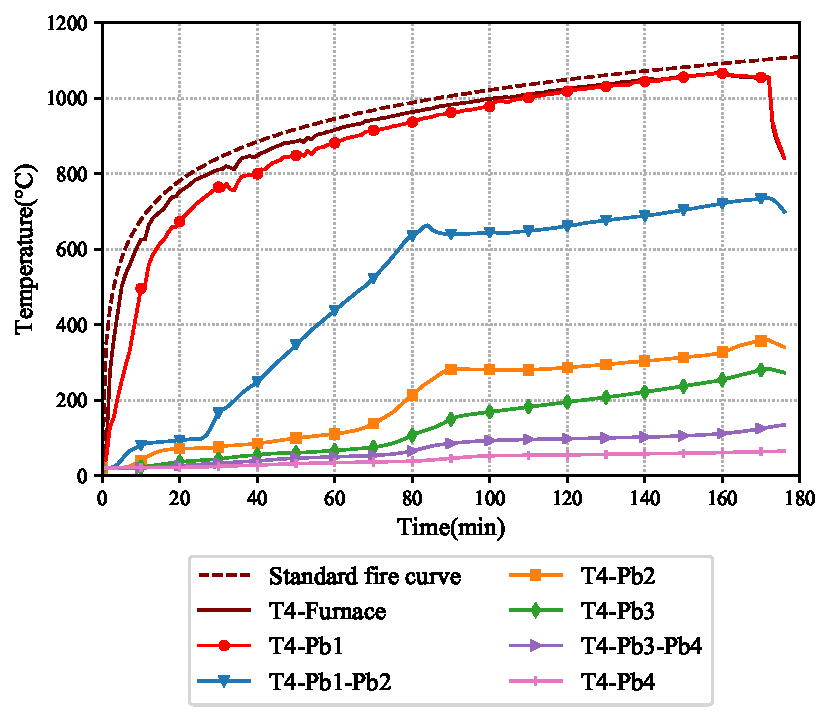
\includegraphics[width=7cm,height=6cm]{T4-Plasterboard} & 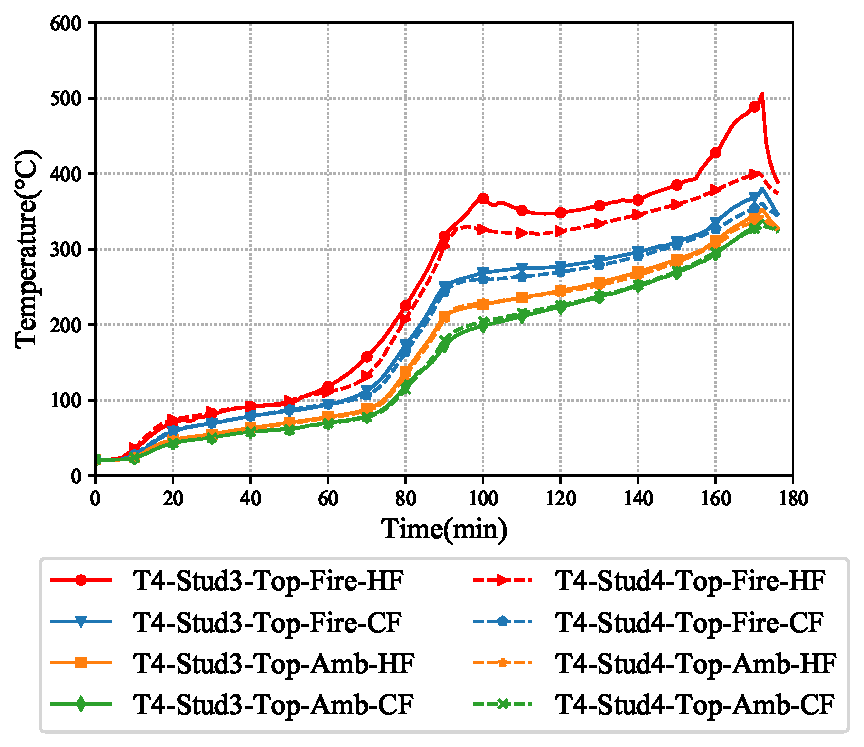
\includegraphics[width=7cm,height=6cm]{T4-Stud3-4-Top} \\
			(a) & (b) \\
		\end{tabular} 
		\caption{Plasterboard and stud time-temperature curves of Test-T4 (a) Average plasterboard temperatures (b) Stud3 temperatures}
		\label{fig:T4-PB-Stud}
\end{figure}

The stud time-temperature curves from the fire test are shown in \Cref{fig:T4-PB-Stud}~(b). All the stud hot and cold flanges time-temperature curves were less than 100\degree C till 50 min from the start of fire test. A steep increase in the T3-Stud4-Top-Fire-HF was observed after 60 min reaching a first peak of 325\degree C at 100 min of fire test. After this, there was a dip in the time-temperature curve reaching a lowest of 320\degree C at 114 min. This dip was due to the reduction in temperature of 5\degree C and was attributed as a result of plateau region witnessed in the Pb2 plasterboard time-temperature curve. This further evolves to a maximum of 491\degree C at the end of fire test. The corresponding cold flange time-temperature curve T4-Stud3-Top-Fire-CF followed a similar trend in correlation with the hot flange T4-Stud3-Top-Fire-HF. The maximum temperature recorded by T4-Stud3-Top-Fire-CF was 371\degree C at the end of fire test. The difference between the fire side hot and cold flanges was 120\degree C. However, the ambient side hot and cold flanges exhibited a similar behaviour throughout the fire test. The temperatures of T4-Stud3-Top-Amb-HF and CF were 348\degree C and 332\degree C with a temperature difference of 16\degree C only. This infers that the temperature difference between the fire side hot and cold flanges is larger in comparison with the ambient side hot and cold flanges in non-insulated cavity walls. This behaviour was also reflected in Test-T1 and T2.
\begin{figure}[!htbp]
	\centering
		\begin{tabular}{cc}
			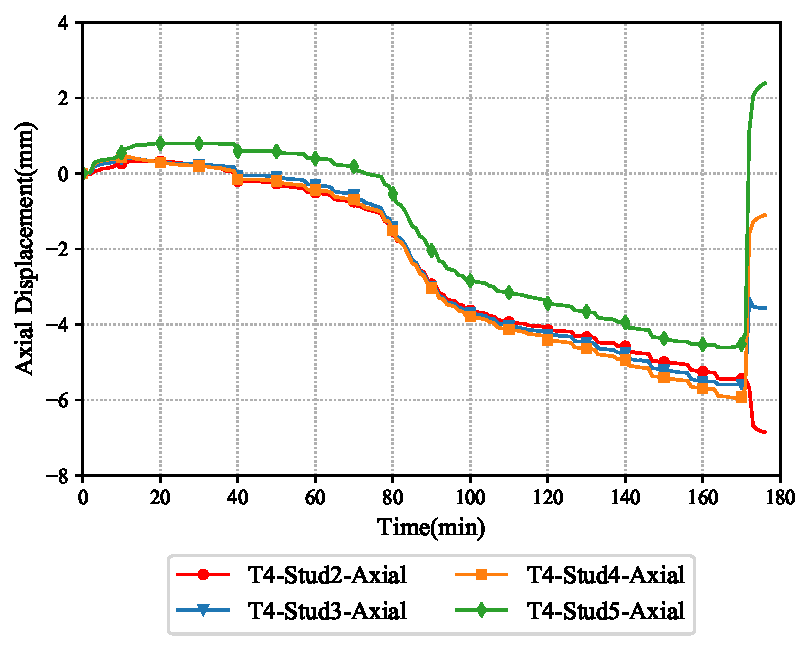
\includegraphics[width=7cm,height=6cm]{T4-Axial} & 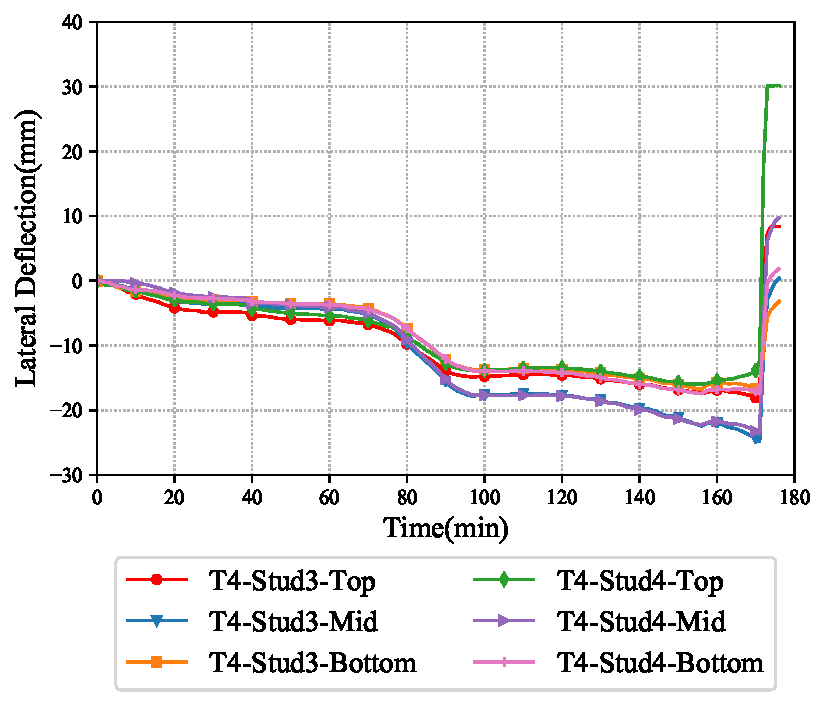
\includegraphics[width=7cm,height=6cm]{T4-Lateral} \\
			(a) & (b) \\
		\end{tabular} 
		\caption{Axial displacement and lateral deflection curves from Tests-T4 (a) Time vs Axial displacement (b) Time vs Lateral deflection curves}
		\label{fig:T4-Axial-Lateral}
\end{figure}

The axial displacement versus time plots is shown in \Cref{fig:T4-Axial-Lateral}~(a). Axial displacement in studs were less than -2 mm till 80 min of the fire test after which the curves exhibited a gradual increase reaching a maximum of -5.95 mm at 169 min of fire test. This indicates thermal expansion in the studs during fire test. After this the curve exhibited a sudden reversal reaching -1.59 mm indicating shortening and failure of the studs. Lateral deflection versus time plots are shown in \Cref{fig:T4-Axial-Lateral}. In accordance with the axial displacement plots the lateral deflections in the test wall was less than -10 mm in all the studs till 80 min of fire test. The curve exhibited gradual increase in the reaching a maximum of -24.43 mm at 171 min in T4-Stud3-Mid. After this the curve reversed indicating a sudden reversal reaching a peak of 0.35 mm indicating structural failure of studs. The curve T4-Stud4-Top also recorded a deflection of 30.15 mm at the end of fire test which confirm structural failure in the test wall. The behaviour of axial displacement curves from this fire test was similar to the other non-cavity insulated double stud LSF wall fire Tests-T1 to T3 wherein the maximum axial displacement during the fire test was less than 10 mm. The lateral deflection curves also exhibited a similar behaviour in all non-cavity insulates double stud wall fire tests.


\section{Fire Test-T5}

Test-T5 was conducted on double stud wall with cavity insulation on both rows of the studs. \cref{fig:T5-plan-details} shows the test wall details and construction. 90 mm Lipped Channel Sections (LCS) were used as studs made from G550 steel with a Base Metal Thickness (BMT) of 0.95 mm. Glass fibre insulation bats of 75 mm were used as cavity insulation with a density of 11 kg/m\(^3\). A 20 mm air gap was present between both the rows of studs.
\begin{figure}[htbp]
	\centering
		\begin{tabular}{c}
			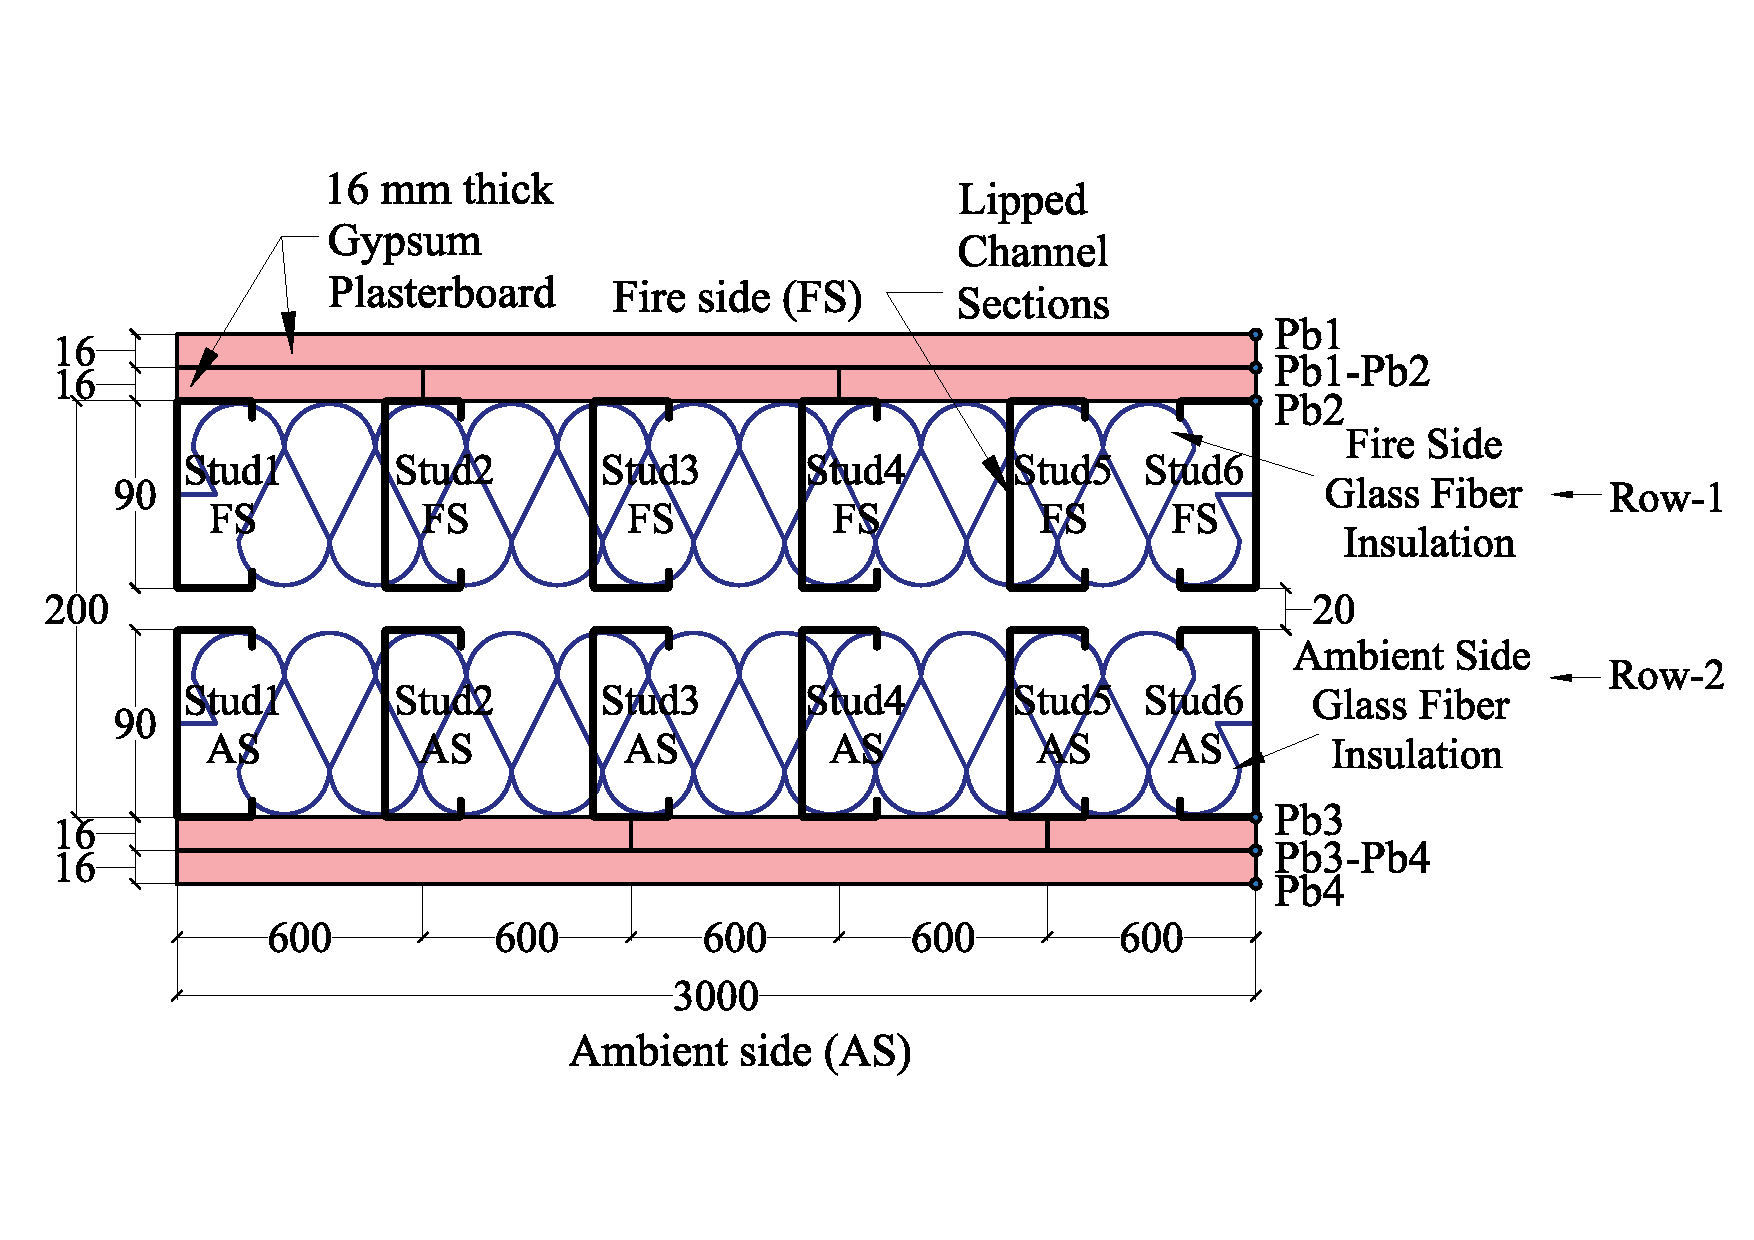
\includegraphics[width=9cm, height=5cm]{T5-plan.pdf} \\
			(a)\\ 
			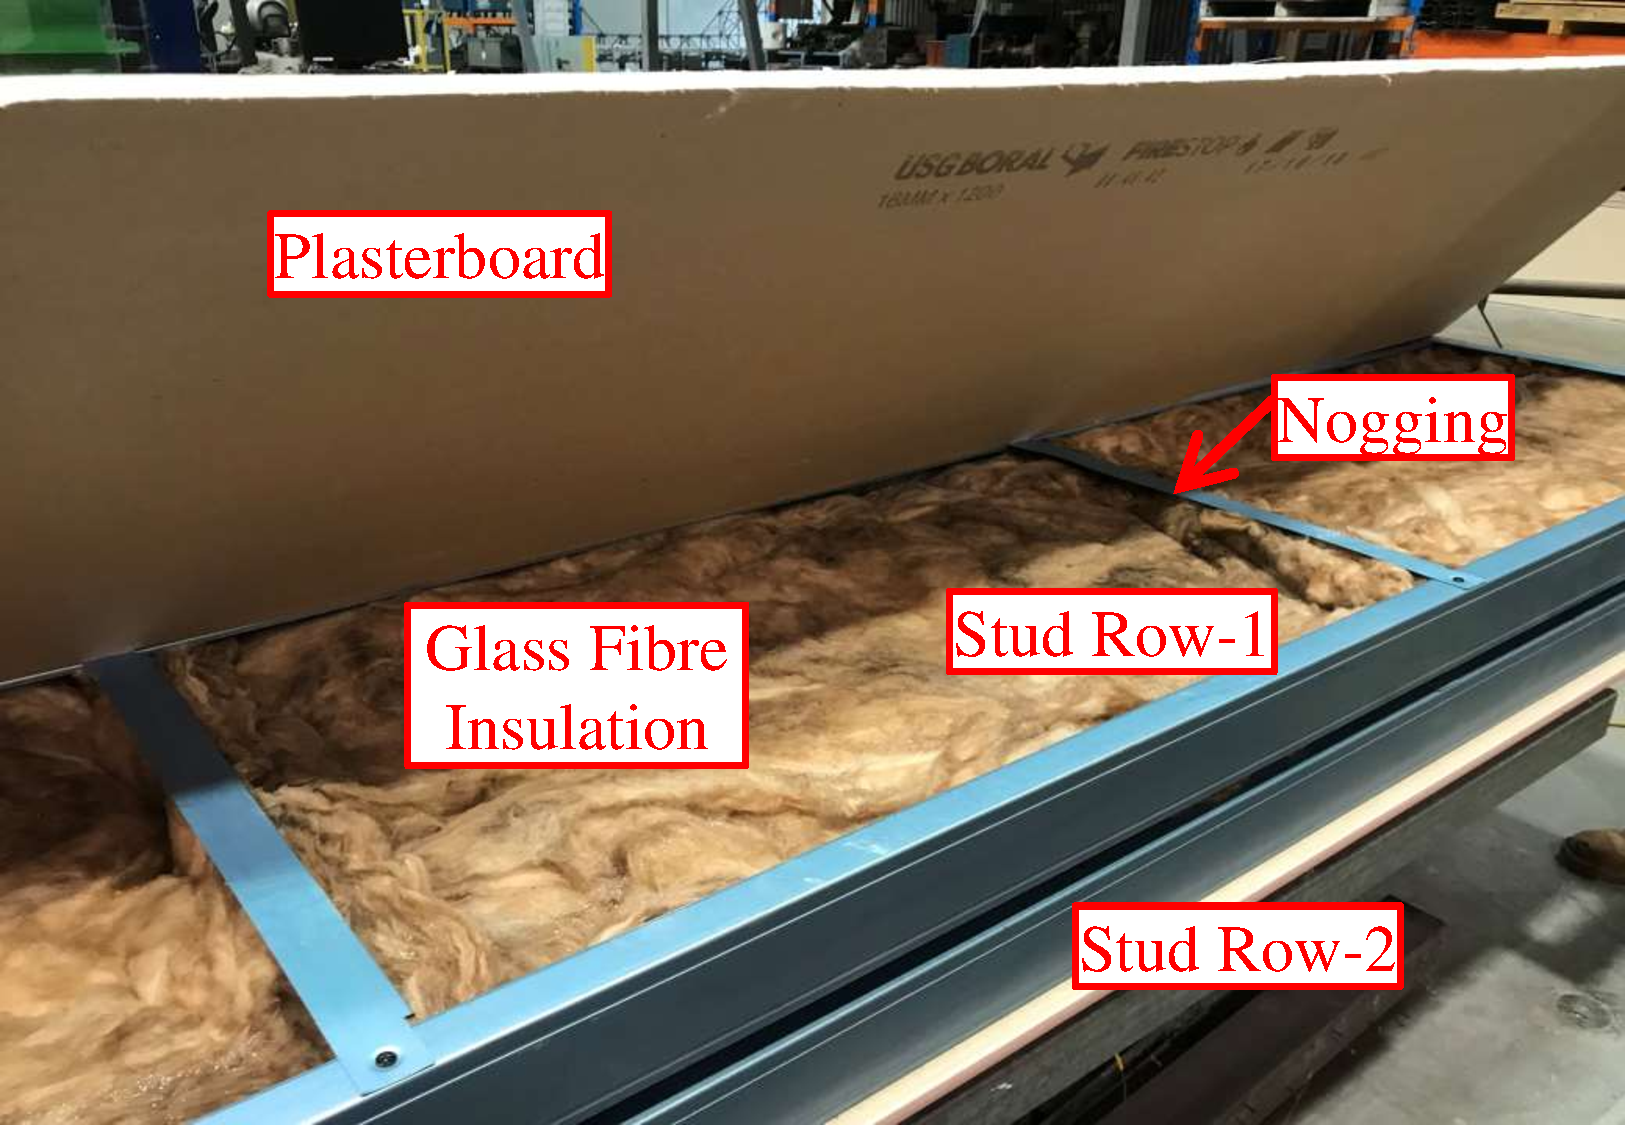
\includegraphics[width=8cm, height=5cm]{T5-construction.pdf}\\
			(b) \\
		\end{tabular}
		\caption{(a) Typical cross-section of Test-T5 (b) Construction of test wall-T5}
		\label{fig:T5-plan-details}
\end{figure}   

After 13 min from the start of fire test, plasterboard joint compound fall off from the fire side plasterboard surface was noticed. No significant changes to the ambient side plasterboard was noticed till 40 min. Mild smoke was visible at 43 min of fire test signifying the calcination of the fire exposed plasterboard. Evaporation of the chemically bound water molecules from the plasterboard resulting in vapours was not noticeable due to the presence of cavity insulation. Dark and heavy smoke patches were noticeable on the top right corner of the test wall indicating the entrapment of heat on the fire side of the test wall at 56 min. The test wall survived for 76 min and the test was concluded due to structural inadequacy failure of the studs. Post fire test examination of the test wall revealed significant local buckling on the fire side studs as shown in \cref{fig:T5-failure}. Also, the cavity insulation on the ambient side of the wall was unaffected. This shows that the heat was trapped only on the fire side of the test wall. However, the ambient side studs were also unaffected and no buckling was observed. This also confirms the entrapment of heat on the fire side of the test wall which was the main contributor for the fire side stud buckling.
\begin{figure}[!htbp]
	\centering	
		\begin{tabular}{cc}
			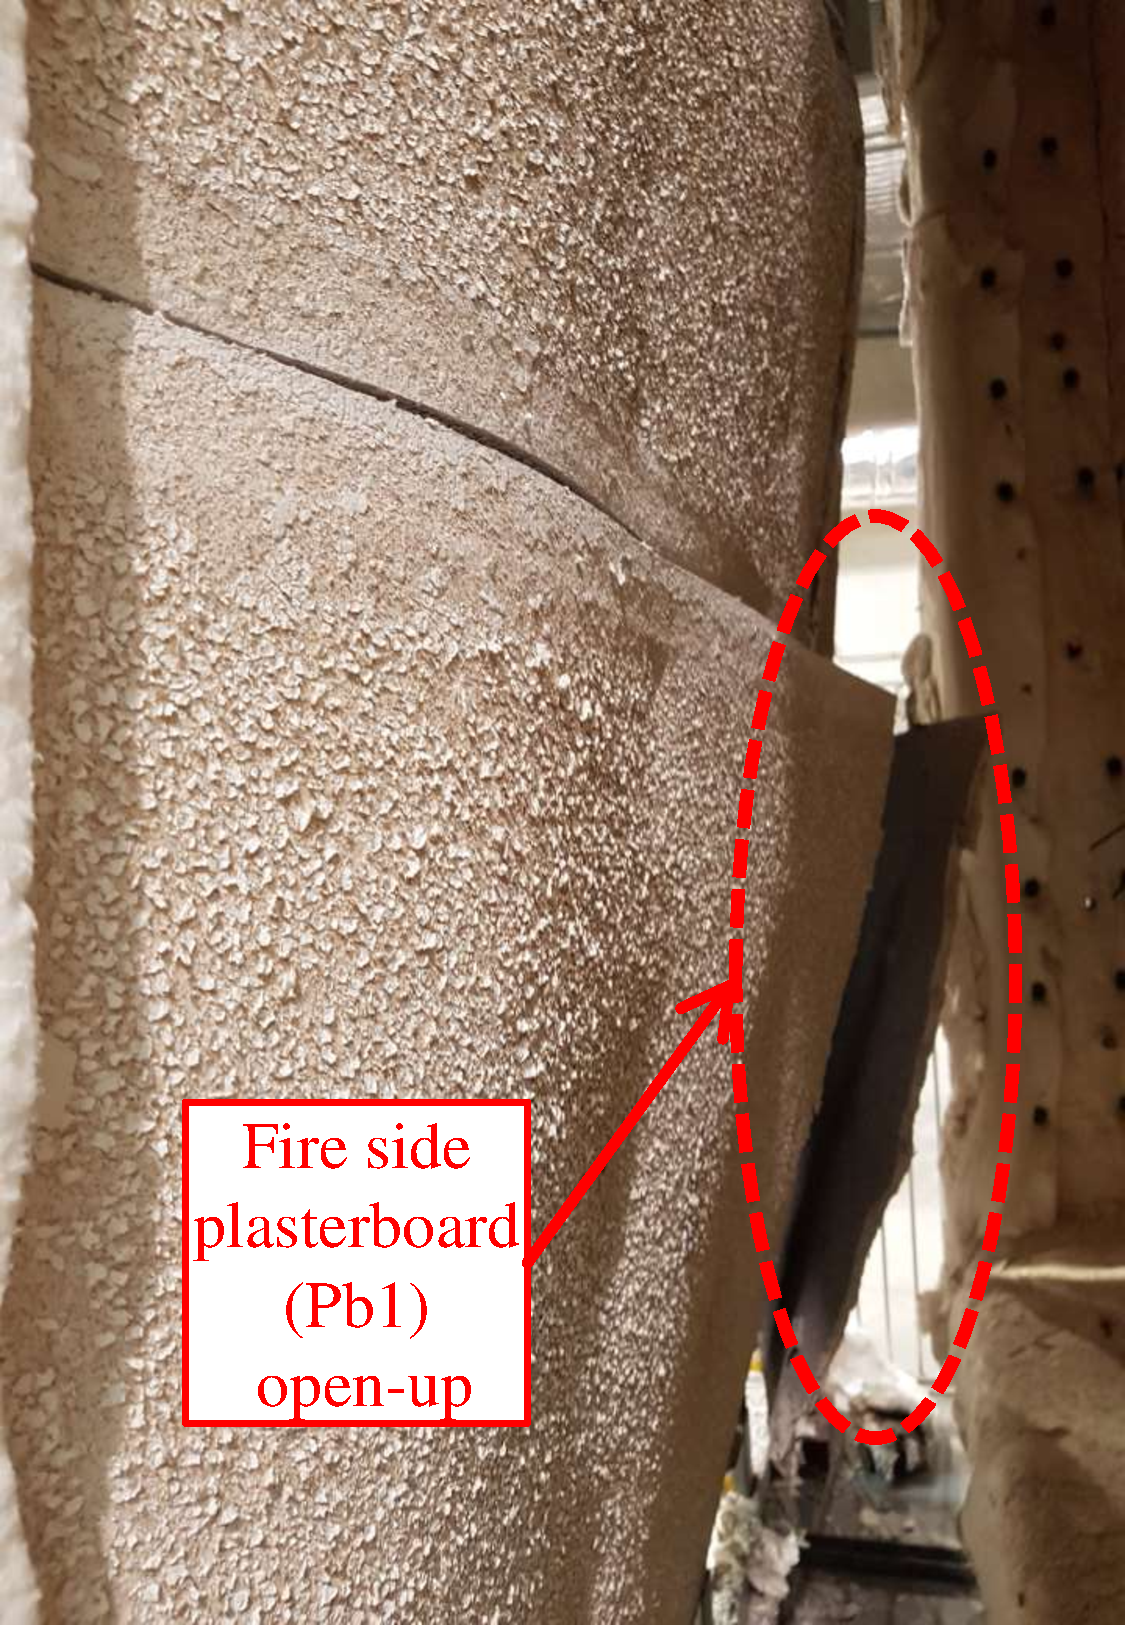
\includegraphics[scale=0.25]{T5-fireside.pdf} & 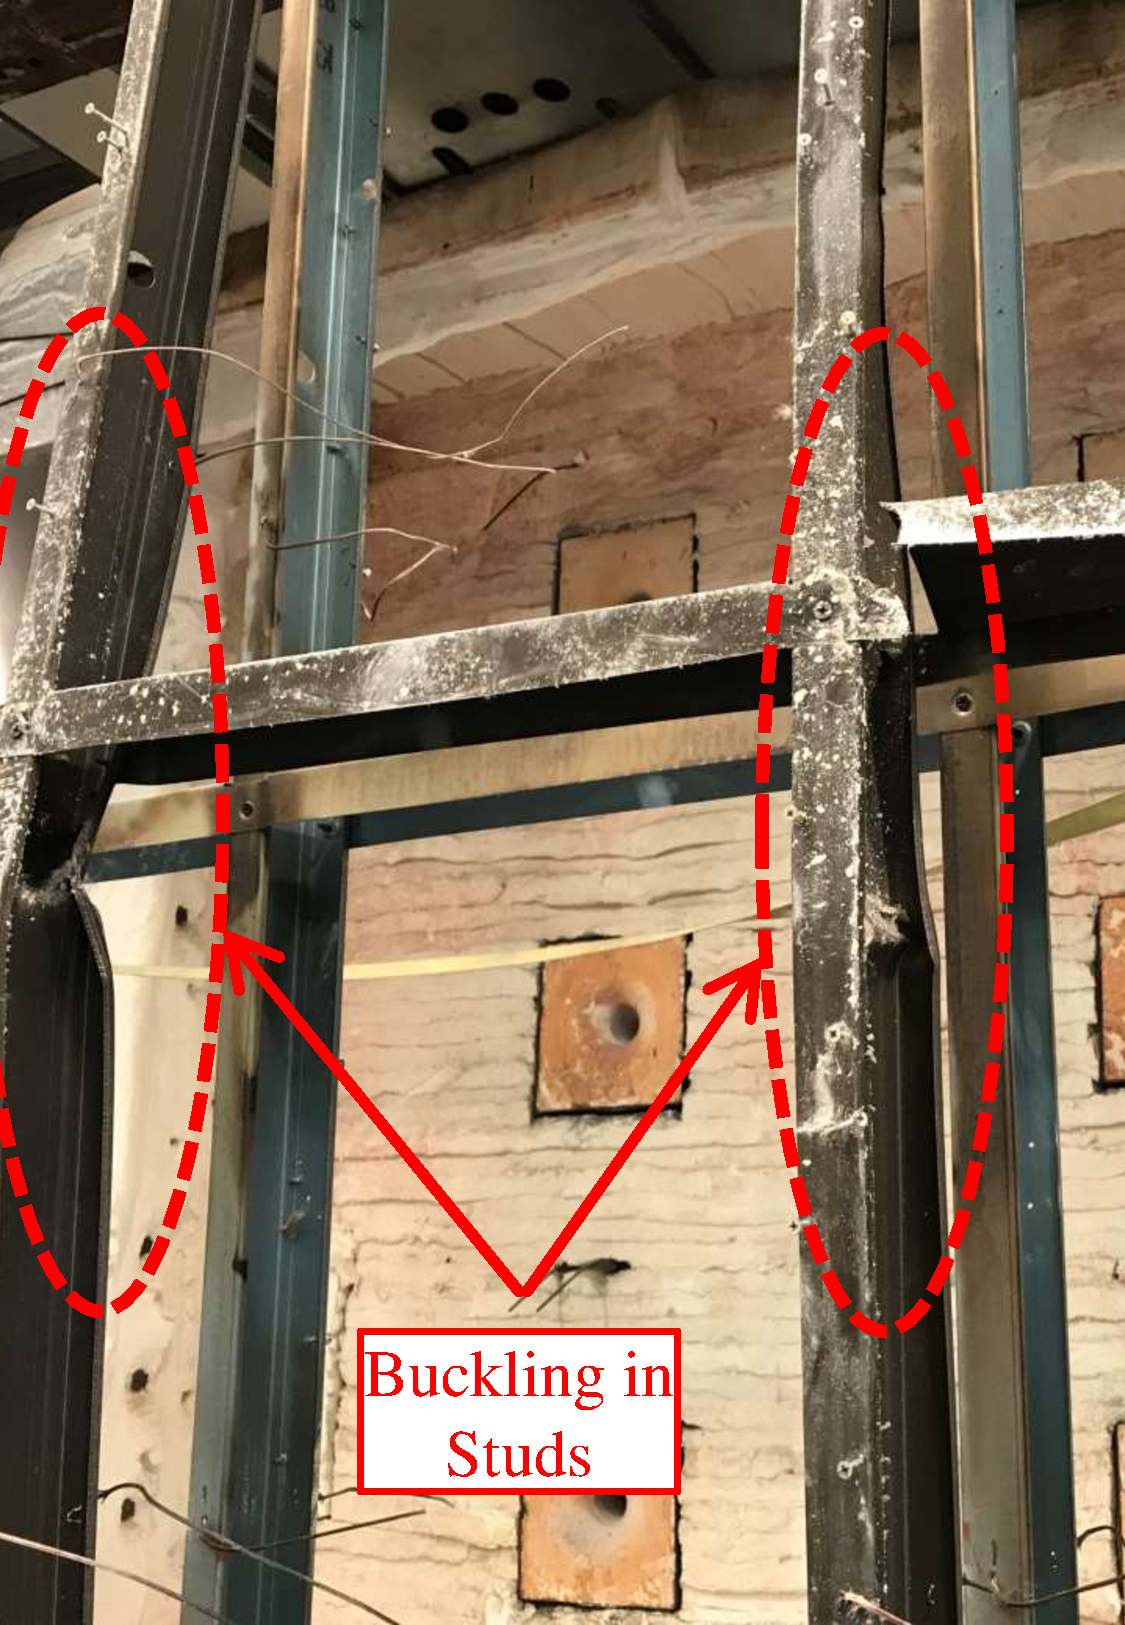
\includegraphics[scale=0.25]{T5-stud_buckling.pdf} \\
			(a) & (b) \\
			\end{tabular}
		\caption{Test-T5 wall failure (a) Fire side plasterboard open up; (b) Buckling in fire side studs}
		\label{fig:T5-failure}
\end{figure}
It is evident form the post fire test investigation that severe opening of the plasterboard is due to the entrapment of heat on fire exposed side of the test wall only. The glass fibre cavity insulation prevents the hot gases to enter into the 20 mm cavity thereby resulting in reduced temperature on the ambient side studs. The time-temperature, axial displacement and lateral deflection curves from the full-scale fire test are presented and discussed next.

\subsection{Test-T5 Results and Discussion}

The average plasterboard time-temperature curves are presented in \cref{fig:T5-time-temperature} (a). The fire side plasterboard interface time-temperature curve (Pb1-Pb2) exhibits a flat region till 25 min from the start of the fire test. Then the curve exhibits a steep rise till the end of fire test reaching a maximum of 621\degree C. This implies the calcination of the fire exposed plasterboard, thereby transferring the heat to the next surface which is the fire side plasterboard interface (Pb1-Pb2). But this trend is not noticeable in the fire side cavity surface (Pb2). The time-temperature curve is nearly flat till 65 min of the fire test after which the curve takes a steep increase and reaches 425 \degree C. This implies that the heat from the fire side interface (Pb1-Pb2) is not effectively dissipated into the cavity because of the presence of cavity insulation. This is also evident from the ambient side plasterboard time-temperature curves. The ambient side cavity surface (Pb3), ambient side plasterboard interface (Pb3-Pb4) and the ambient side surface (Pb4) did not exhibit any significant variation in the time-temperature curve and recorded temperatures less than 200\degree C till the end of fire test. This is less than the limiting temperature for the insulation failure criteria proving the absence of insulation failure in the fire test. This behaviour of the time-temperature curve also supports our earlier claim of the heat being entrapped on the fire side surfaces only.
\begin{figure}[!htbp]
	\centering	
		\begin{tabular}{cc}
			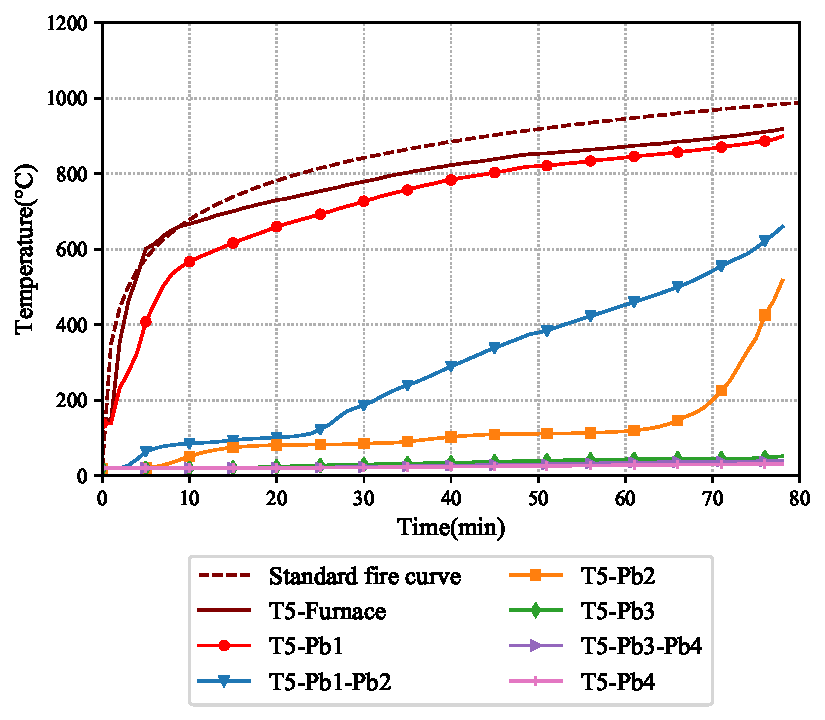
\includegraphics[width=7cm,height=6cm]{T5-Plasterboard.pdf} & 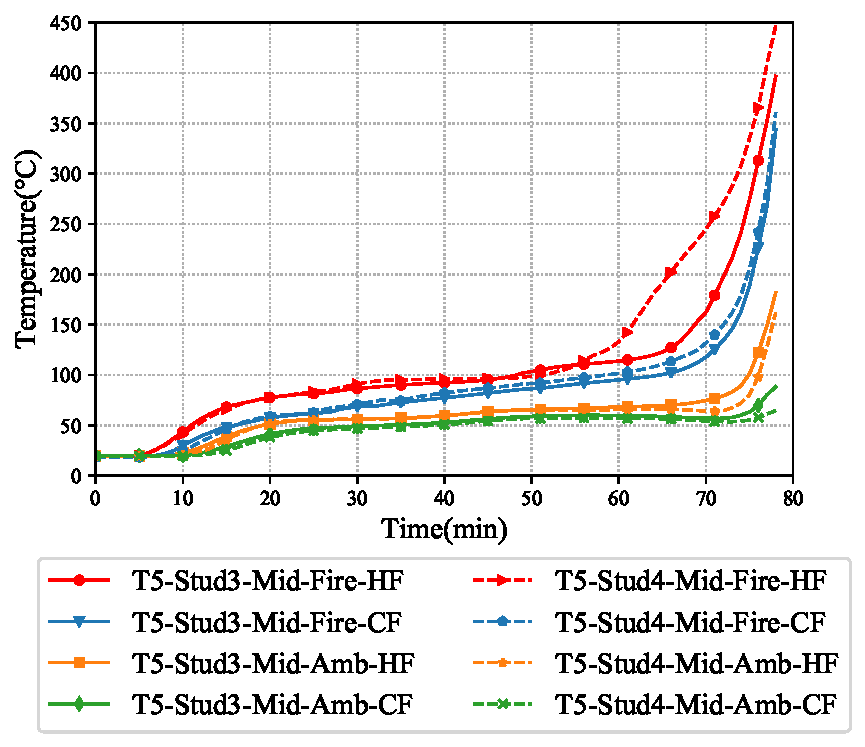
\includegraphics[width=7cm,height=6cm]{T5-Stud3-4-Mid.pdf} \\
			(a) & (b) \\
			\end{tabular}
		\caption{Test-T5 (a) Time versus Axial Displacement; (b) Time versus Lateral Deflection}
		\label{fig:T5-time-temperature}
\end{figure}

Likewise, the stud time-temperature curves are presented in \cref{fig:T5-time-temperature} (b) and also exhibits a similar pattern to that of the fire side plasterboard interface (Pb1-Pb2). The fire exposed stud hot flange time-temperature curve (T5-Stud4-Mid-Fire-HF) exhibited only a progressive increase till 55 min of the fire test. The recorded temperature was well below 150\degree C. There was a sudden increase in the time-temperature curve from 60 min and the curve reached a maximum of 447\degree C at the end of fire test. The corresponding cold flange (T5-Stud4-Mid-Fire-CF) exhibited a similar trend reaching a maximum of 360\degree C. However, the temperatures on the ambient side hot and cold flanges are comparatively lesser than the fire side studs. The ambient hot and flange time-temperature curves (T5-Stud4-Mid-Fire-HF and CF) were well below 100\degree C till 70 min of the fire test. The time-temperature curves on the ambient side row of studs recorded temperatures less than the limiting temperature for the insulation failure in plasterboards. Also, the temperatures on the ambient side studs were less than the limiting temperatures for studs proposed by past researchers under load bearing conditions \citet{Feng2003,Gunalan2013a}. 
\begin{figure}[!htbp]
	\centering	
		\begin{tabular}{cc}
			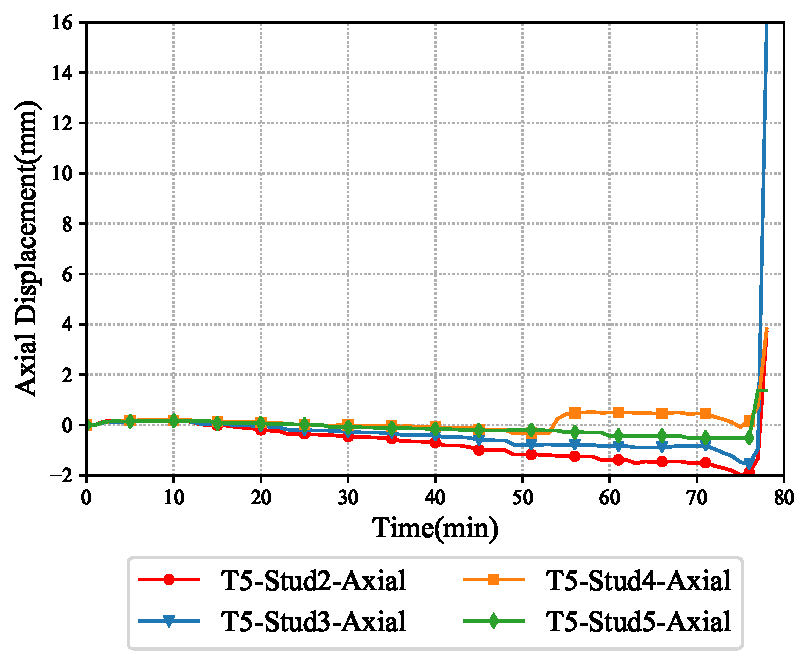
\includegraphics[width=7cm,height=6cm]{T5-Axial.pdf} & 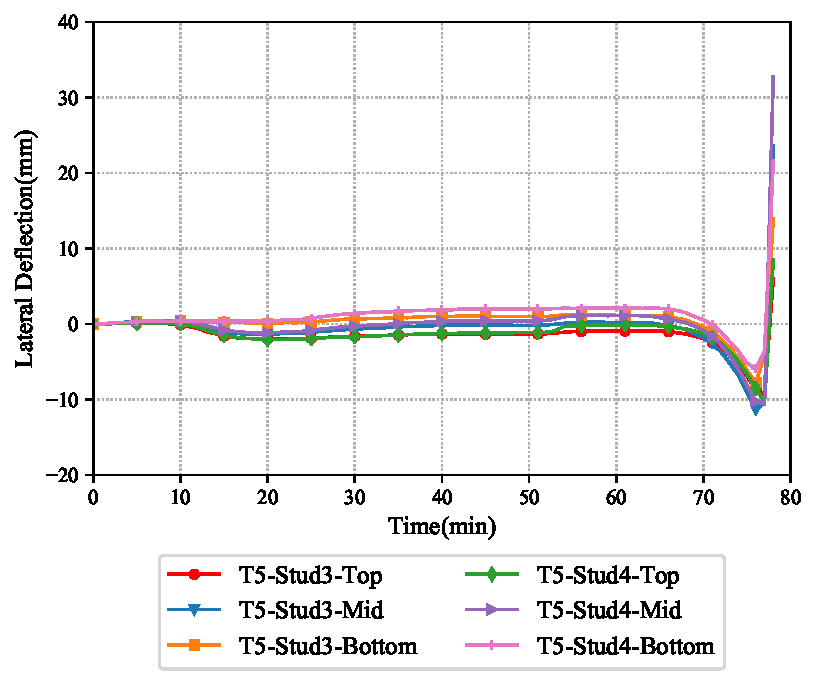
\includegraphics[width=7cm,height=6cm]{T5-Lateral.pdf} \\
			(a) & (b) \\
			\end{tabular}
		\caption{Test-T5 time-temperature curves (a) Average Plasterboard; (b) Stud4-Mid}
		\label{fig:T5-displacement}
\end{figure}

The axial displacement and lateral deflection curves from the fire test are shown in Figures.~\ref{fig:T5-displacement}(a) and (b). No significant axial displacement was observed till 50 min from the start of fire test. Small axial expansion was observed after which the curve propagates to a maximum axial displacement of -2 mm. The curve then indicated a reversal and a maximum displacement of 15.86 mm was observed indicating severe axial compression indicating the end of fire test. This indicates that the effect of temperature entrapment plays a significant role in the structural failure of double stud LSF walls with cavity insulation. This is also evident from the time versus lateral deflection curves. No significant lateral deflection was observed till 65 min of fire test. After this the test wall started to bow inwards causing a deflection of -10 mm. After this the test wall bowed outwards resulting in a lateral deflection of 32.72 mm at the end of fire test. This implies that the severity of thermal bowing is less in cavity insulated double stud LSF walls. 

\section{Fire Test-T6}

Test-T6 was a repeat test and was conducted on double stud LSF wall with cavity insulation on both sides as shown in \Cref{fig:T5-plan-details}~(a). As the fire Test-T5 resulted in an FRL of 76 min, which is 100 min less than the corresponding non-cavity insulated wall fire test, the Test-T5 was repeated to determine the validity of the previous full-scale fire test conducted with the same configuration. The test specimen was constructed similar to Test-T5 and full-scale fire test was conducted. After 28 min from the start of fire test, joint compound fall-off from the fire side plasterboard surface (Pb1) was observed. Mild smoke was visible form the top right corner of the test specimen at 46 min of the fire test.  
\begin{figure}[!htbp]
	\centering	
		\begin{tabular}{cc}
			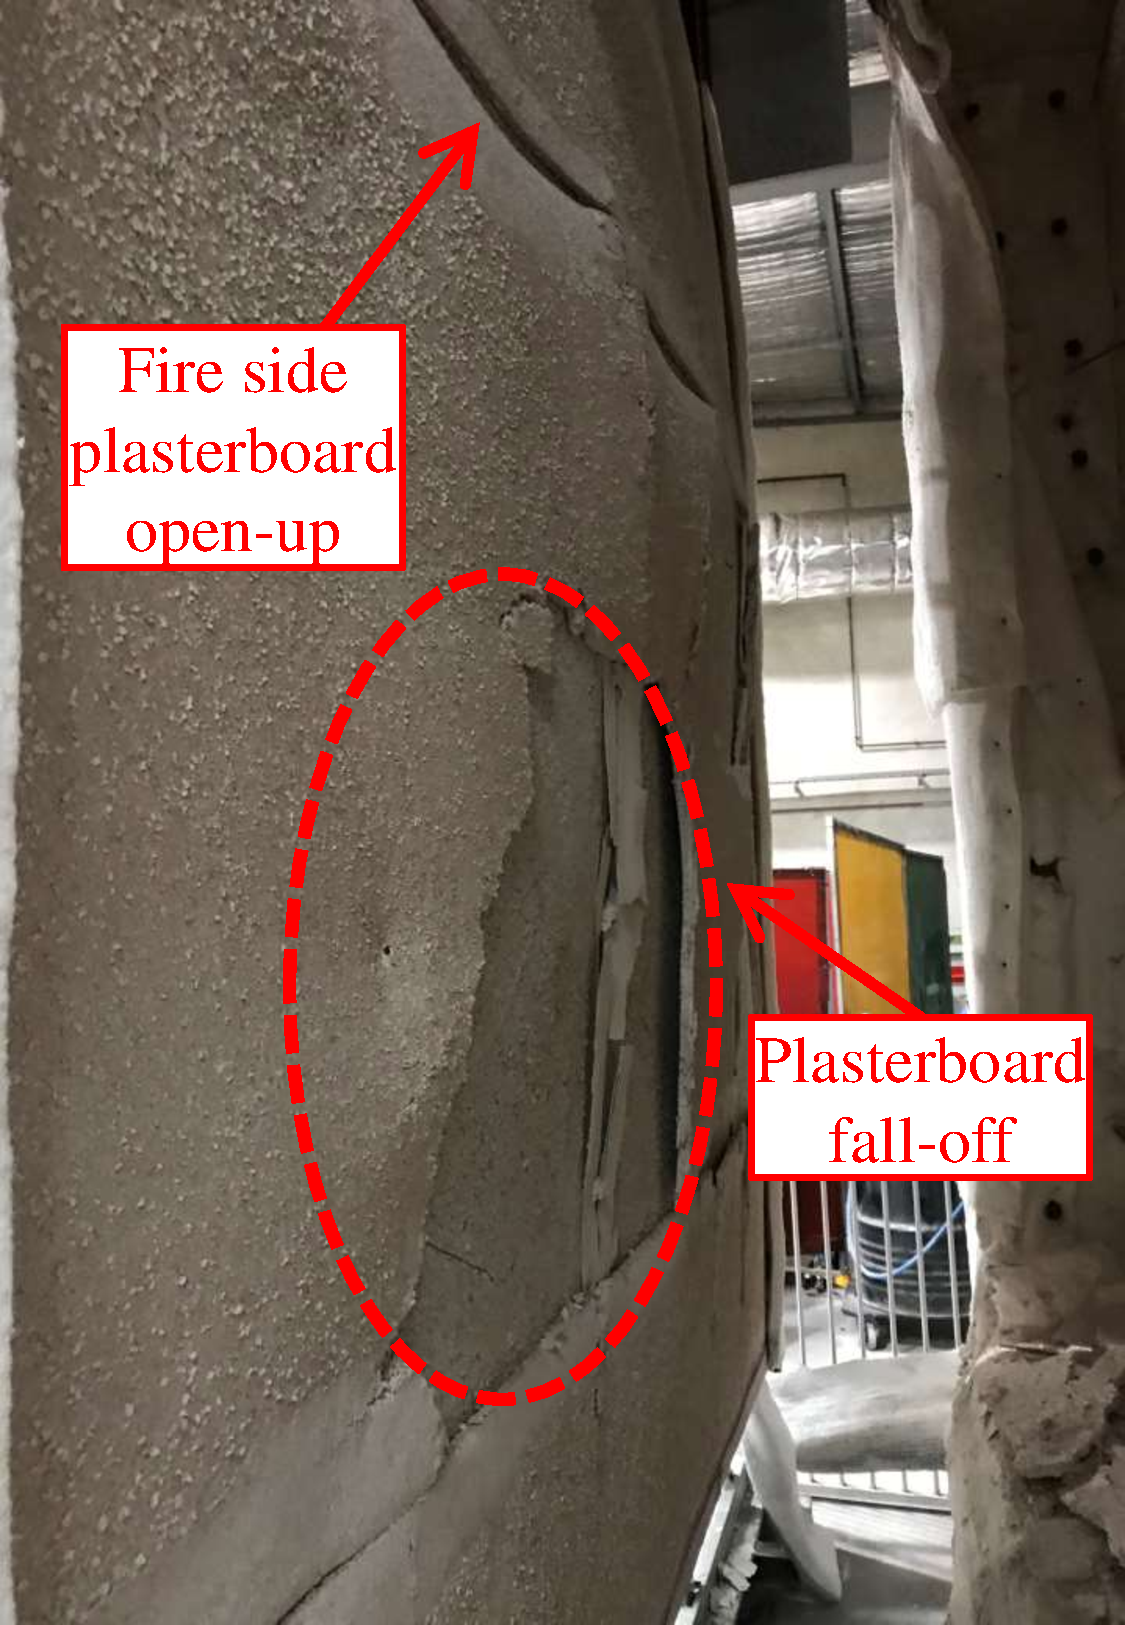
\includegraphics[scale=0.25]{T6-fireside.pdf} & 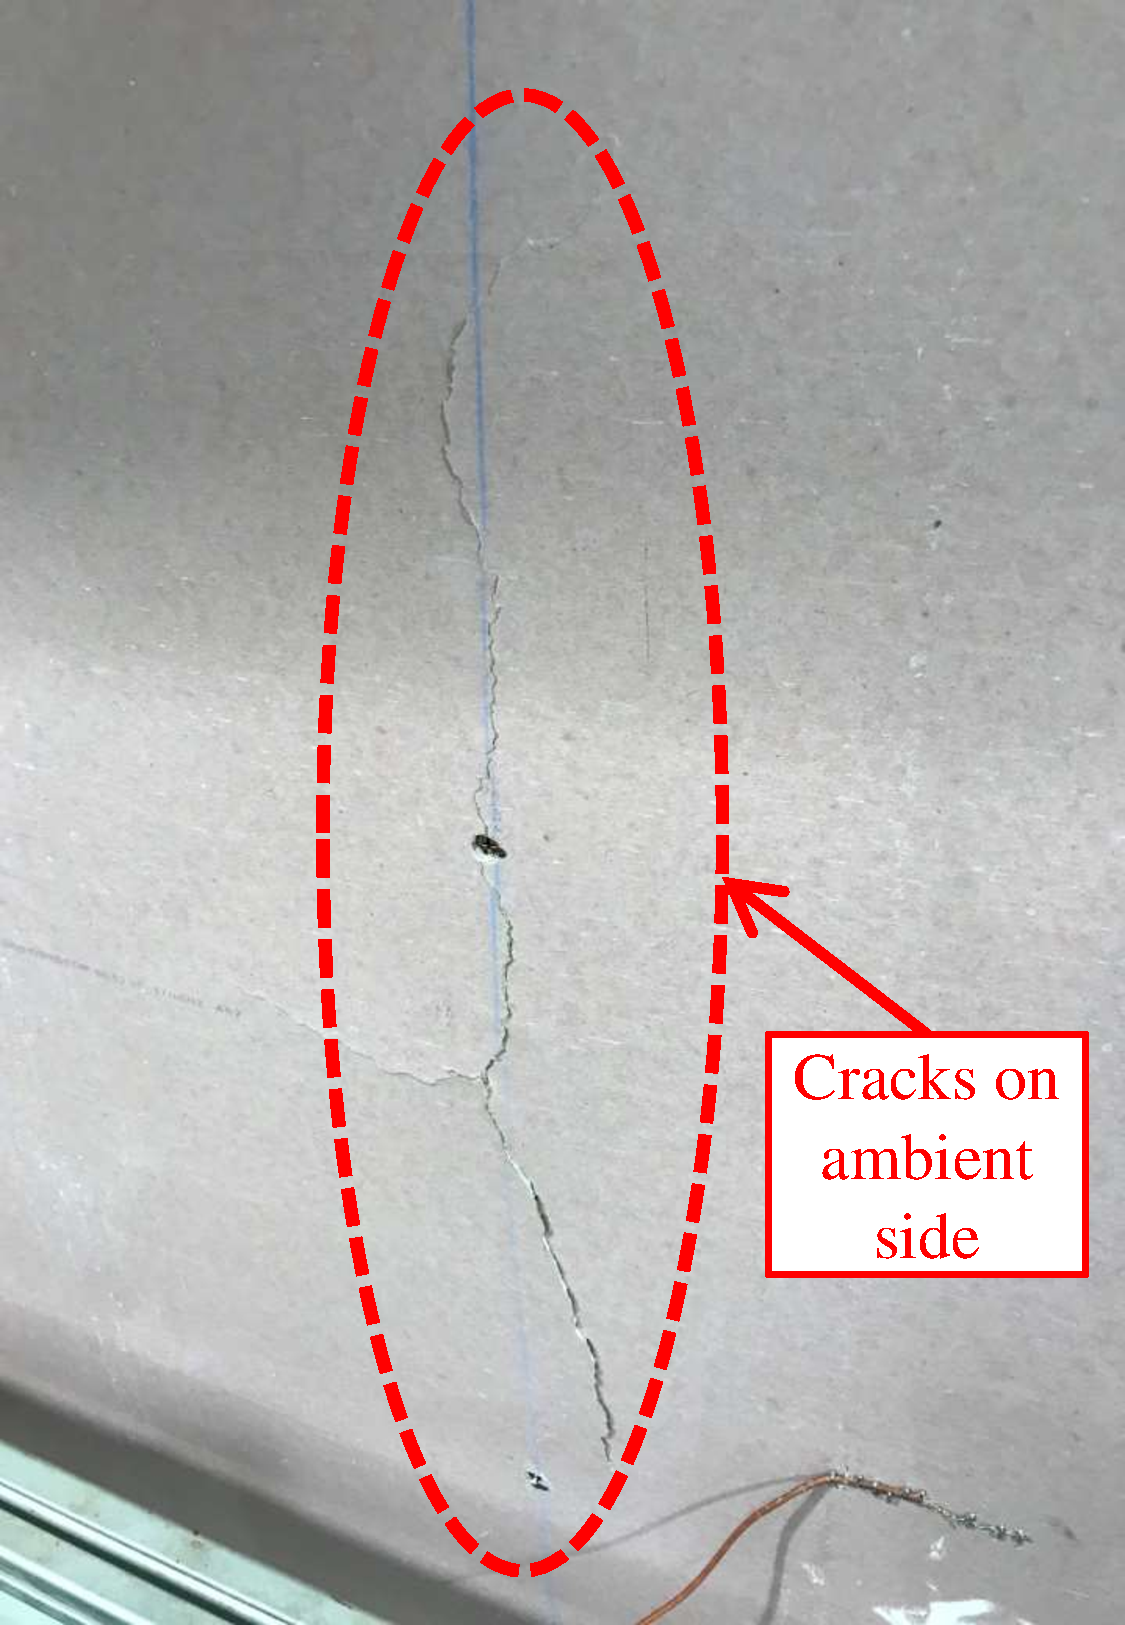
\includegraphics[scale=0.25]{T6-ambient_cracks.pdf} \\
			(a) & (b) \\
			\end{tabular}
		\caption{Test-T6 wall failure (a) Fire side plasterboard open up; (b) Cracks on ambient side plasterboard}
		\label{fig:T6-fireside}
\end{figure}
\begin{figure}[!htbp]
	\centering	
		\begin{tabular}{cc}
			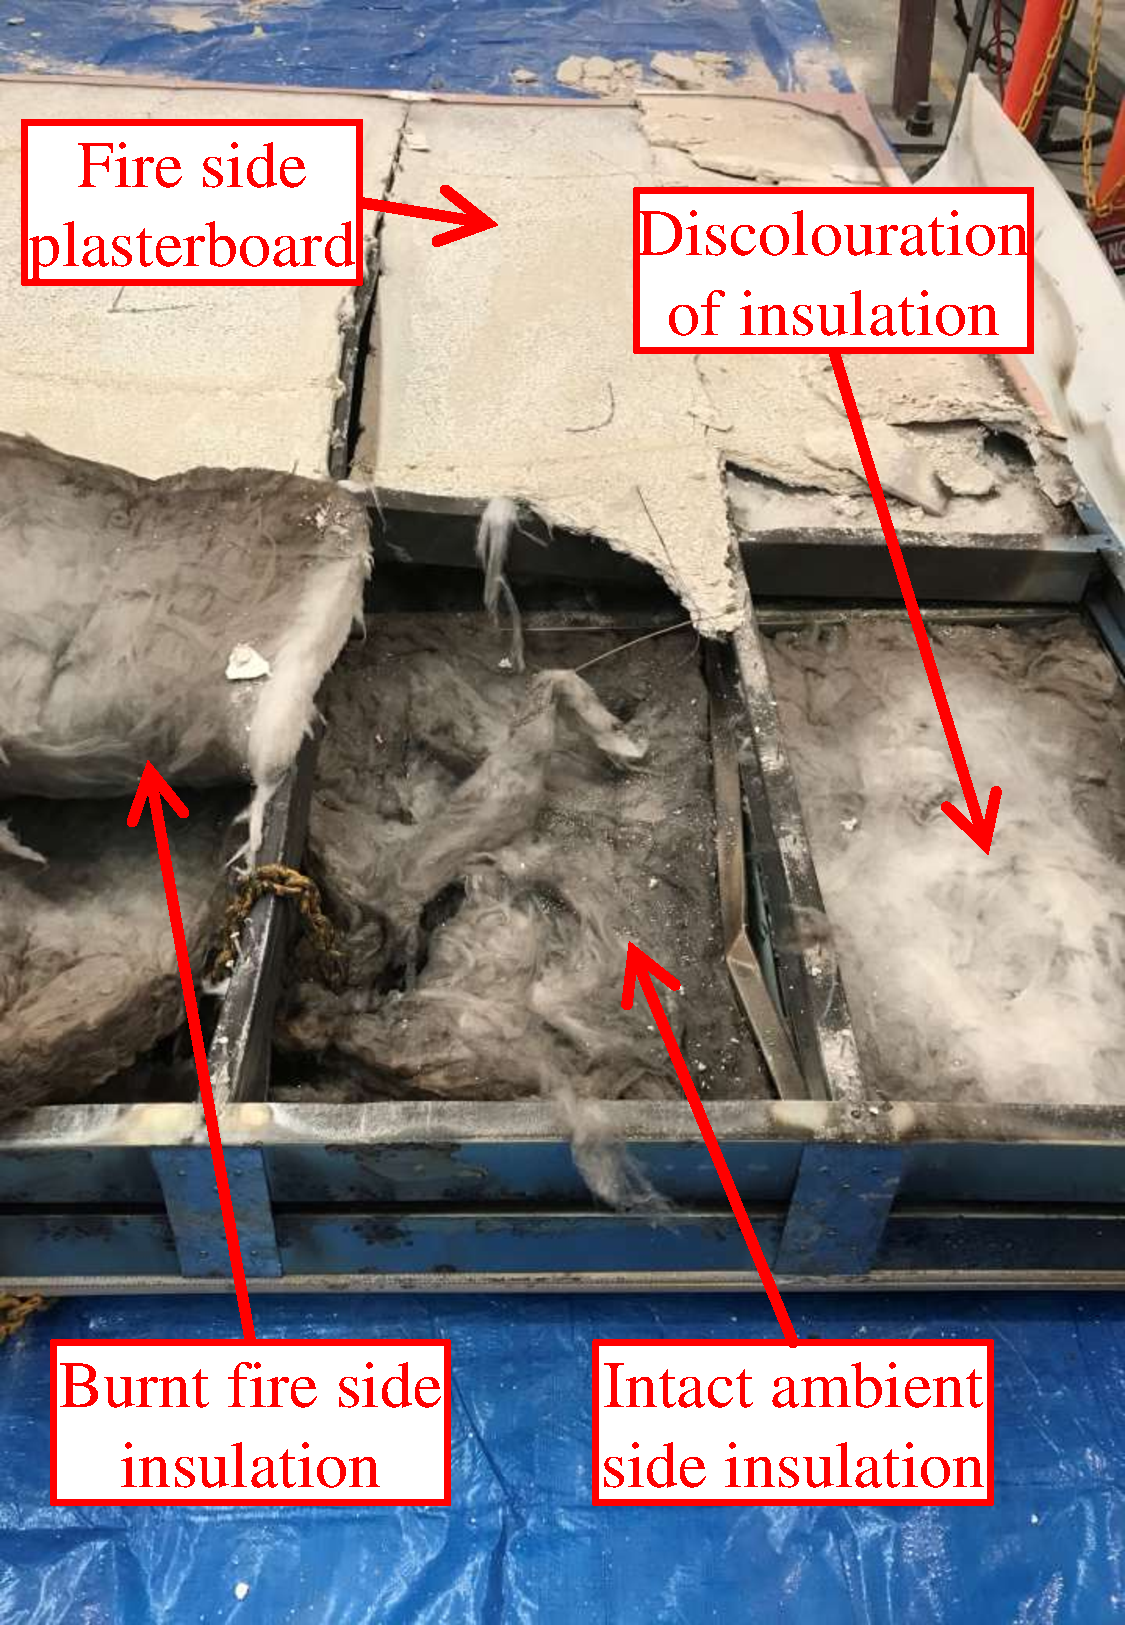
\includegraphics[scale=0.25]{T6-insulation_burnt.pdf} & 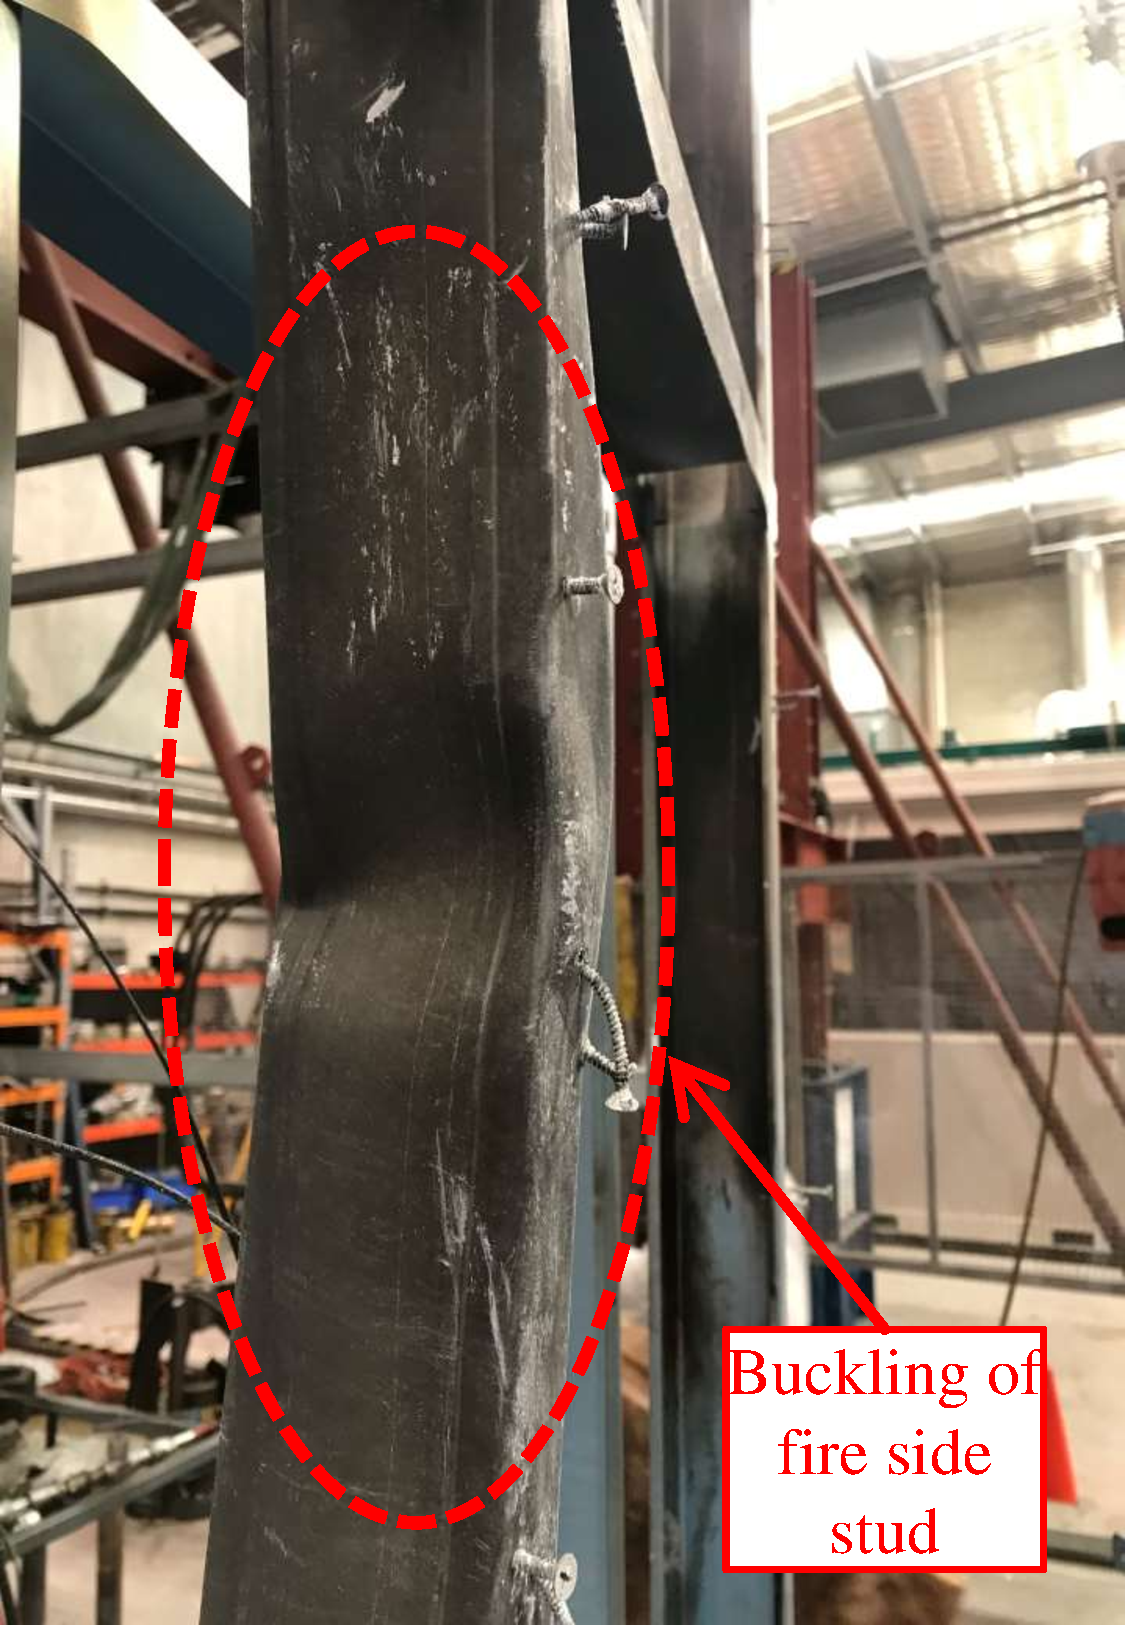
\includegraphics[scale=0.25]{T6-buckling.pdf} \\
			(a) & (b) \\
			\end{tabular}
		\caption{Test-T6 wall failure (a) Discolouration of insulation; (b) Buckling in fire side stud}
		\label{fig:T6-failure}
\end{figure}

Intensity of the smoke increased at 50 min and stopped at 59 min intimating the calcination process on the fire side plasterboards. At 59 min the Pb1 joint compound was completely burnt and a small opening was noticeable on the fire side plasterboard when observed through the thermal camera. Again at 77 min high intensity smoke was observed on the top right corner of the test specimen and continued till 82 min, showing the calcination of second plasterboard layer on the fire side (Pb2). Multiple cracks were observed on the fire side plasterboards at 86 min and was visible through the thermal camera images. Later, at 91 min the test wall could not withstand the applied axial load and failed due to structural inadequacy criteria. Cracks on the ambient side plasterboard (Pb4) was noticeable at the time of failure due to excessive lateral deflection in studs as shown in \Cref{fig:T6-fireside}~(a). Post fire test investigations showed the discolouration in the fire and ambient side glass fibre insulation. Also, after stripping the plasterboards, local buckling of the fire side studs as shown in \Cref{fig:T6-failure}~(b) was noticeable and found to be the dominant failure mode.

\subsection{Test-T6 Results and Discussion}

The plasterboard time-temperature curves from Test-T6 is shown in \Cref{fig:T6-time-temperature}~(a). The fire side plasterboard interface Pb1-Pb2 recorded temperatures less than 100\degree C till 25 min of fire test. A sudden increase in the Pb1-Pb2 time-temperature curve was noticeable after 25 min from the start of fire test reaching a maximum of 800\degree C at the end of fire test (91 min). However, similar to the previous Test-T5 the fire side cavity (T6-Pb2) temperatures were well below 200\degree C till 69 min of the fire test after which the T6-Pb2 time-temperature curve exhibited a sudden increase reaching a peak of 570\degree C at 82 min indicating the calcination of the second plasterboard layer on the fire exposed side of the test wall. After this, there was a small dip in the time-temperature curve dropping down to 518\degree C at 91 min indicating a reduction in temperature of 52\degree C in 9 min. Plasterboard open-up letting the hot gases inside the cavity could be attributed to the drop in time-temperature curve on the fire side cavity plasterboard surface (T6-Pb2). The ambient side plasterboard cavity (T6-Pb3), ambient side plasterboard interface (T6-Pb3-Pb4) and ambient side (Pb4) surface temperatures were well below 100\degree C till the end of fire test. This indicates the absence of insulation failure in the test wall.
\begin{figure}[!htbp]
	\centering	
		\begin{tabular}{cc}
			\includegraphics[width=7cm,height=6cm]{T6-Plasterboard.pdf} & \includegraphics[width=7cm,height=6cm]{T6-Stud3-4-Top.pdf} \\
			(a) & (b) \\
			\end{tabular}
		\caption{Test-T6 time-temperature curves (a) Average Plasterboard; (b) Stud3 and 4-Top}
		\label{fig:T6-time-temperature}
\end{figure}

Stud time-temperature curves also exhibited a similar pattern in comparison with the fire test results from Test-T5. All the stud hot and cold flange temperatures were well below 200\degree C till 69 min which is in correlation with the T6-Pb2 plasterboard time-temperature curve. After this the hot flange (T6-Stud4-Top-Fire-HF) exhibited a sudden rise reaching a peak of 544\degree C at the end of fire test. However, the maximum temperature recorded at T6-Stud3-Top-Fire-HF was 547\degree C at 85 min after which there is a dip in the time-temperature curve. The T6-Stud3-Top-Fire-HF recorded 507\degree C at 91 min which is a 40\degree C drop in 6 min interval. This behaviour is attributed by the time-temperature curve dip in the fire side plasterboard as a result of plasterboard open-up as shown in \Cref{fig:T6-time-temperature}~(a). 
\begin{figure}[!htbp]
	\centering	
		\begin{tabular}{cc}
			\includegraphics[width=7cm,height=6cm]{T6-Axial.pdf} & \includegraphics[width=7cm,height=6cm]{T6-Lateral.pdf} \\
			(a) & (b) \\
			\end{tabular}
		\caption{Test-T5 (a) Axial displacement; (b) Lateral deflection versus time}
		\label{fig:T6-displacement}
\end{figure}

The axial displacement experienced by the test wall was less and also similar to Test-T5. Maximum axial displacement recorded was -0.12 mm at 80 min of fire test in T6-Stud4-Axial. A sudden axial contraction was noticeable at 81 min whereby the axial displacement reached 2.68 mm at 85 min. Sudden failure due to buckling of fire side studs was the reason behind this failure after which the load is transferred to the ambient side studs. This is evident from the undulations in the axial displacement curve at 82 min as shown in \Cref{fig:T6-displacement}~(a). The test wall could not withstand the applied axial load any further and failed due to structural adequacy at 91 min. Lateral deflection versus time curves also exhibited a similar behaviour to Test-T5. No significant lateral deflection was noticeable till 70 min of the fire test after which the curve reached a maximum of -24.33 mm near at T6-Stud3-Mid (1500 mm from top of specimen) at 80 min indicating inward thermal bowing towards the furnace. Outward thermal bowing was observed after 80 min wherein the curve reached a maximum of 17.83 mm at the end of fire test.

\section{Fire Test-T7}

To determine the effect of cavity insulation position in double stud LSF walls, Test-T7 was conducted with cavity insulation on the ambient row of studs only. The test frame dimensions were maintained similar to that of Test-T5 and similar test setup and boundary conditions were used. However, the effective cavity width including the 20 mm gap was 110 mm in this fire test. The cavity insulation was placed away from the fire side to allow the passage of heat into the cavity so that the entrapment of heat on the fire side do not occur as in Test-T5. 
\begin{figure}[!htbp]
	\centering
		\includegraphics[scale=0.30]{T7-plan}
		\caption{Test-T7 details}
		\label{fig:T7-plan}
\end{figure}

After 11 min from the start of fire test mild smoke was witnessed from the top left corner of the test wall. The smoke continued without any change in  intensity until 28 min of fire test. Water droplets dripping from the bottom of the test wall near Stud1 was also noticed due to the moisture movement in plasterboard. Water patches were also visible on the ambient side plasterboard surface (Pb4) at mid-height of the test wall. Sever plasterboard open up was observed on the fire exposed side as shown in \cref{fig:T7-failure} (a). Post fire test examination revealed the occurrence of buckling on the fire side studs only as shown in \cref{fig:T7-failure} (b). Another important observation was that the cavity insulation was completely intact after the fire test. 
\begin{figure}[!htbp]
	\centering	
		\begin{tabular}{cc}
			\includegraphics[scale=0.25]{T7-fireside.pdf} & \includegraphics[scale=0.25]{T7-buckling.pdf} \\
			(a) & (b) \\
			\end{tabular}
		\caption{Test-T7 wall failure (a) Fire side plasterboard open up; (b) Buckling in fire side studs}
		\label{fig:T7-failure}
\end{figure}

\subsection{Test-T7 Results and Discussion}

The time-temperature curves from Test-T7 corresponding to average plasterboard is presented in \cref{fig:T7-time-temperature} (a). Similar to Test-T5 the fire side plasterboard time-temperature curve was flat till 25 min of fire test after which the curve exhibited a steep rise reaching a maximum temperature of 718\degree C at the end of fire test. But the corresponding fire side plasterboard cavity time-temperature curve (T7-Pb2) was flat till 60 min of the fire test. A gradual increase in the time-temperature curve was noticed after that till the end of fire test reaching a maximum of 400\degree C at the end of fire test. This indicates that similar to Test-T5 the cavity insulation did not allow the heat to pass into the ambient side of the test wall. This is further evident from the time-temperature curves of the ambient side plasterboard. The time-temperature curve on the ambient side cavity (Pb3), ambient side plasterboard interface (Pb3-Pb4) and the ambient side plasterboard surface (Pb4) all resulted in temperatures less than 100 \degree C till the end of fire test.
\begin{figure}[!htbp]
	\centering	
		\begin{tabular}{cc}
			\includegraphics[width=7cm,height=6cm]{T7-Plasterboard.pdf} & \includegraphics[width=7cm,height=6cm]{T7-Stud3-4-Mid.pdf} \\
			(a) & (b) \\
			\end{tabular}
		\caption{Test-T7 time-temperature curves (a) Average Plasterboard; (b) Stud4-Mid}
		\label{fig:T7-time-temperature}
\end{figure}

The time-temperature curve on the studs as shown in \cref{fig:T7-time-temperature} (b) also exhibited a similar behaviour in comparison with Test-T5. All the hot and cold flange temperatures of the studs were well below 100\degree C till 50 min of fire test. After 50 min the fire side hot flange (T7-Stud3-Mid-Fire-HF) time-temperature curve upsurged rapidly to attain a maximum of 438\degree C at the end of fire test. The corresponding cold flange T7-Stud3-Mid-Fire-HF recorded a maximum of 363\degree C. The ambient side hot and cold flanges were well below 100\degree C till 70 min of fire test after which the time-temperature curve T7-Stud3-Mid-Amb-HF gradually increased to reach a maximum of 263\degree C at the end of fire test. However, the T7-Stud3-Mid-Amb-CF recorded temperatures well below 200\degree C till the end of fire test.  
\begin{figure}[!htbp]
	\centering	
		\begin{tabular}{cc}
			\includegraphics[width=7cm,height=6cm]{T7-Axial.pdf} & \includegraphics[width=7cm,height=6cm]{T7-Lateral.pdf} \\
			(a) & (b) \\
			\end{tabular}
		\caption{Test-T7 (a) Time versus Axial Displacement; (b) Time versus Lateral Deflection}
		\label{fig:T7-displacement}
\end{figure}

The axial displacement and lateral deflection plots are presented in Figs.\ref{fig:T7-displacement} (a) and (b). There was no significant axial displacement in the studs till 65 min of the fire test. This is in correlation with the low time-temperature profile in the studs. The maximum axial displacement due to thermal expansion was -4.26 mm only at 80 min of fire test after which load reversal occurred resulting in an axial shortening of +10.52 mm at the end of fire test. The fire test was concluded after 81 min due to structural inadequacy as the test wall could not withstand the applied axial load. 

\section{Fire Test-T8}

Test-T8 was conducted on a double stud LSF wall made of 90 mm deep studs with noggings at 1 m spacing and a plasterboard layer between the two rows of stud (effective cavity depth of 90 mm). The fire test was conducted for 240 min. Water droplets were visible in the top left corner of the ambient side plasterboard (Pb4) after 35 min of fire exposure. The fire side plasterboard layers were completely calcinated, however, the plasterboard layer between the studs (Pb3) and those on the ambient side (Pb4 and Pb5) were intact until the end of the fire test (\Cref{fig:T8-fireside-buckling}(a)). 
\begin{figure}[!htbp]
	\centering
		\begin{tabular}{cc}
			\includegraphics[width=7cm,height=5.5cm]{T8-fireside} & \includegraphics[scale=0.25]{T8-buckling} \\ 
			(a) & (b)  \\ 
		\end{tabular} 
		\caption{Test-T8 wall frame after the fire test (a) Pb1-Plasterboard fall-off (b) Local buckling of studs}
		\label{fig:T8-fireside-buckling}
\end{figure}

\subsection{Test-T8 Results and Discussion}

\Cref{fig:T8-PB-Stud-Lateral} (a) shows the average plasterboard time-temperature curves from Test-T8. The fire side plasterboard temperature (Pb1) agreed reasonably well with the standard fire curve until about 180 min of the fire test. Excessive plasterboard fall-off on the fire side after 164 min is evident from the sudden rise in the T8-Pb1-Pb2 time-temperature curve, reaching the fire side curve. The ambient side plasterboard temperatures were less than 100\degree C till the end of the fire test, as evident from the T8-Pb5 curves shown in \Cref{fig:T8-PB-Stud-Lateral} (c). This confirms the absence of insulation failure in the test until 240 min.
\begin{figure}[!htbp]
	\centering
		\begin{tabular}{cc}
			\includegraphics[width=7cm,height=6cm]{T8-Plasterboard} & \includegraphics[width=7cm,height=6cm]{T8-Studs-3-4-Mid}\\
			(a) & (b)  \\ 
			\includegraphics[width=7cm,height=6cm]{T8-Plasterboard-5} & \includegraphics[width=7cm,height=6cm]{T8-Lateral} \\ 
			(c) & (d)  \\ 
		\end{tabular} 
		\caption{Temperature and lateral deflection versus time curves from Test-T8 (a) Average plasterboard temperature (b) Stud3 and Stud4 temperatures (c) Ambient side plasterboard (Pb5) temperature and (d) Lateral deflection}
		\label{fig:T8-PB-Stud-Lateral}
\end{figure}

The stud time-temperature curves from Test-T8 are shown in \Cref{fig:T8-PB-Stud-Lateral} (b). The fire side hot flange (T8-Stud3-Mid-Amb-HF) recorded a maximum temperature of 985\degree C at 240 min while the ambient side hot flange T8-Stud3-Mid-Amb-HF recorded a maximum temperature of 718\degree C at 240 min. The corresponding cold flange temperatures (T8-Stud3-Mid-Fire-CF and T8-Stud3-Mid-Amb-CF) were 968\degree C and 674\degree C. Such high stud temperatures are unlikely to be reached in load bearing fire tests as confirmed by many load bearing fire tests (\citet{Feng2005,Chen2012a,Kodur2013,Magarabooshanam2019}). Although this test wall was tested under non-load bearing conditions, local buckling of hot and cold flange elements was observed on both fire and ambient side studs (\Cref{fig:T8-fireside-buckling}~(b)). The local buckling was due to the high temperatures experienced on all the stud hot and cold flanges where the intact ambient side plasterboard acts as an additional load. The lateral deflection versus time curve was nearly flat and recorded -7 mm at 100 min of fire test. It then increased to a maximum of -30 mm after 200 min and reversed back to -3 mm as shown in \Cref{fig:T8-PB-Stud-Lateral} (d).

\section{Fire Test-T9}

Test-T9 was conducted on a staggered stud LSF wall with 90 mm deep studs (cavity depth of 150 mm) and lined with two layers of 16 mm gypsum plasterboards. The studs are arranged in a staggered pattern with every alternative stud at 600 mm centres. The staggered stud LSF wall configuration used for the Test-T9 is shown in \Cref{fig:T9-plan}. This test was conducted under non-load bearing conditions to investigate the time-temperature profile staggered stud LSF wall configuration. After 20 min, mild smoke was observed on the top right corner of the test wall. Water droplets were visible due to the process of plasterboard calcination in the top left corner on the ambient side. \Cref{fig:T9-fireside-bowing}(a) shows the fire side (Pb1) of test wall after the test, which reveals a significant plasterboard fall-off on the fire side. 
\begin{figure}[!htbp]
	\centering
		\includegraphics[scale=0.45]{T9-plan}
		\caption{Test-T7 details}
		\label{fig:T9-plan}
\end{figure}

This is due to the excessive thermal bowing of the test wall as shown in \Cref{fig:T9-fireside-bowing} (b). The average time-temperature curves of the plasterboard and stud surfaces from Test-T9 are summarised in Figures~\ref{fig:T9-PB-Stud-Lateral}~(a)~to~(c). The time-temperature curve of fire side plasterboard interface T9-Pb1-Pb2 was nearly flat for the initial 25 min after which the curve exhibited a steep rise, reaching 693\degree C at 88 min. Then the curve became a plateau and showed only a gradual increase during 80 to 120 min. This observation is similar to Test-T2 and is caused by the wider cavity (150 mm) producing a natural convection within the cavity in comparison with Test-T1 with a smaller cavity depth (76 mm). A reduced time-temperature profile is also visible on the fire side cavity T9-Pb2. This behaviour is also caused by the discontinuous stud arrangement in staggered stud wall. The plateau region observed in the authors' previous study \citet{Magarabooshanam2019} was also present in the plasterboard T9-Pb1-Pb2 and T9-Pb2 time-temperature curves confirming the earlier claim. However, the duration of the plateau region was shorter in comparison with the authors' previous study. This is partly due to the increased cavity depth of 200 mm used in the previous study in comparison with the cavity depth of 150 mm used in this study.  
\begin{figure}[!htbp]
	\centering
		\begin{tabular}{ccc}
			\includegraphics[scale=0.2]{T9-fireside} & \includegraphics[scale=0.2]{T9-bowing} & \includegraphics[scale=0.2]{T9-stud_buckling} \\ 
			(a) & (b) & (c)  \\ 
		\end{tabular} 
		\caption{Test-T9 wall frame after the fire test (a) Pb1-Plasterboard fall-off (b) Thermal bowing (c) Local buckling failure of studs}
		\label{fig:T9-fireside-bowing}
\end{figure}

\subsection{Test-T9 Results and Discussion}

The highest temperature recorded on the fire side hot flange (T9-Stud3-Mid-Fire-HF) was 840\degree C at 187 min. As the plasterboard provides no passive protection to the hot flange of every alternative stud this worsens the situation resulting in excessive inward thermal bowing of -18 mm at 155 min. From 155 min to the end of the fire test the test wall deformed outwards resulting in a lateral deflection of  6 mm at 190 min. This means that a total of 24 mm thermal bowing deformation occurred within the last 35 min. The temperatures of the ambient side Pb4 were less than 100\degree C till the end of the fire test as shown in \Cref{fig:T9-PB-Stud-Lateral}~(c), i.e., no insulation failure. 
 
The fire test was conducted for 190 min after which the test was concluded because of the structural failures of studs (\Cref{fig:T9-fireside-bowing} (c)). The lateral deflection versus time curves also show higher lateral deflection at about 190 min (\Cref{fig:T9-PB-Stud-Lateral} (d)). In staggered stud walls the plasterboard provides lateral restraint to only one flange of the studs. This reduces the restraint offered by plasterboards to the studs in comparison with studs restrained on both flanges. Although this is a non-load bearing wall fire test, the ambient side gypsum plasterboard did not soften and remained in position until the end of the fire test. This meant the self weight of the boards acting as a load on the much weakened studs led to their local buckling failures shown in \Cref{fig:T9-fireside-bowing}(c).
\begin{figure}[!htbp]
	\centering
		\begin{tabular}{cc}
			\includegraphics[width=7cm,height=6cm]{T9-Plasterboard} & \includegraphics[width=7cm,height=6cm]{T9-Stud3-4-Top.pdf}\\
			(a) & (b)  \\ 
			 \includegraphics[width=7cm,height=6cm]{T9-Plasterboard-4} & \includegraphics[width=7cm,height=6cm]{T9-Lateral} \\ 
			(c) & (d)  \\ 
		\end{tabular} 
	\fontsize{10}{1}\textit{Note : Thermocouple T9-Stud3-Mid-Fire-CF malfunctioned.}
		\caption{Temperature and lateral deflection versus time curves from Test-T9 (a) Average plasterboard temperature (b) Stud3 and Stud4 temperatures (c) Ambient side plasterboard (Pb4) temperature and (d) Lateral deflection}
		\label{fig:T9-PB-Stud-Lateral}
\end{figure}

The stud time-temperature curves from Test-T9 are shown in \Cref{fig:T9-PB-Stud-Lateral} (b). The first peak temperature of 470\degree C was recorded at 107 min on the fire side stud hot flange (T9-Stud3-Mid-Fire-HF). It reduced to 449\degree C at 123 min, i.e., 21\degree C drop in 16 min after which the temperature increased gradually. This effect is because the fire side stud hot flange losing heat into the wider cavity. This plateau in the hot flange time-temperature curve is also visible in the fire side cavity plasterboard temperature curve (\Cref{fig:T9-PB-Stud-Lateral} (a)). This is evident from the increased slope in the ambient side cavity (T9-Pb3) time-temperature curve as shown in \Cref{fig:T9-PB-Stud-Lateral} (a). Further, the standard fire curve is also nearly flat during this period resulting in the fire side plasterboard surface to lose heat to the ambient side of the test wall.  

The ambient side stud hot flanges (T9-Stud3-Mid-Amb-HF) did not have the temperature plateau as observed for the fire side stud hot flanges. The peak temperature of T9-Stud3-Mid-Amb-HF was 687\degree C at 190 min. Since the temperatures of the hot and cold flanges were high, even the self-weight of the ambient side plasterboards was sufficient to cause local buckling failures of studs at mid-height (\Cref{fig:T9-fireside-bowing} (c)).

\section{Fire Test-T10}

In continuation to Test-T9 the full-scale fire Test-T10 was also conducted on staggered stud LSF wall. However, this test was conducted under load bearing conditions with glass fibre cavity insulation. From the ambient capacity Test-AT5 which was earlier discussed in \Cref{ch:Ambient}, the axial compression capacity of the test wall was determined to be 68.89 kN and 40\% of the load (27.55 kN) was applied to the test specimen and full-scale fire test was conducted. It is to note that, intermittent omega noggings were provided at 1 m intervals to provide lateral restraints. Conventional LCS noggins are connected through the stud flanges, however the omega noggings were connected through the stud webs to maintain the discontinuous stud arrangements. Detail description about the omega nogging connection were discussed in \Cref{ch:Ambient}, \Cref{fig:AT5-construction}~(a). The test wall configuration and construction details are also shown in \Cref{fig:T10-plan,fig:T10-construction}. Unlike the standard insulation installation process in single stud LSF walls, the cavity insulation was staggered between the studs as shown in \Cref{fig:T10-construction}. This was done to meet the acoustic requirements for the test wall. However, the acoustic rating for the wall was not investigate as the research focus was to investigate the fire performance of the cavity insulated staggered stud LSF wall. 
\begin{figure}[!htbp]
	\centering
		\includegraphics[scale=0.45]{T10-plan}
		\caption{Test-T10 Details}
		\label{fig:T10-plan}
\end{figure}
\begin{figure}[!htbp]
	\centering
		\includegraphics[scale=0.30]{T10-construction}
		\caption{Test-T10 Construction Details}
		\label{fig:T10-construction}
\end{figure}

After 7 min from the start of fire test, smoke was visible on the top right corner of the test specimen. Water droplets were also found to be dripping near the origin of smoke indicating the start of evaporation of free water content from gypsum plasterboard. Mild smoke was visible at 34 min of fire test which then lasted till 74 min of the fire test at the top left and right corners of the test wall specimen. The test wall could not withstand the applied axial load after 85 min from the start of fire test and failed due to structural inadequacy of the studs. 

Post fire test investigation showed small plasterboard fall-off at mid-height of the test specimen on the fire exposed surface. The fire side plasterboard Pb1 experienced localised fall-off while the second plasterboard layer on the fire side (Pb2) was intact. However, significant joint open-up was noticeable on the fire side as shown in \Cref{fig:T10-fireside}~(a). It is to note that, the insulation was burnt only on the fire exposed side. However, due to higher temperature concentration near the studs, discolouration of the insulation was noticeable as shown in \Cref{fig:T10-buckling}~(a). Severe global buckling was noticeable on fire side studs, while no significant buckling on the ambient side studs were noticeable as shown in \Cref{fig:T10-buckling}~(b). This implies that the heat transfer within the cavity is blocked by the glass fibre insulation trapping the heat on the fire side studs only. This is also evident from the intermittent discolouration visible near the stud locations. 
\begin{figure}[!htbp]
	\centering
		\begin{tabular}{cc}
			\includegraphics[scale=0.2]{T10-fireside} & \includegraphics[scale=0.2]{T10-ambient_crack} \\ 
			(a) & (b) \\ 
		\end{tabular} 
		\caption{Test-T10 wall frame after the fire test (a) Pb1-Plasterboard fall-off (b) Crack on ambient side plasterboard (Pb4)}
		\label{fig:T10-fireside}
\end{figure}
\begin{figure}[!htbp]
	\centering
		\begin{tabular}{cc}
			\includegraphics[width=7cm,height=6cm]{T10-insulation_burnt} & \includegraphics[width=7cm,height=6cm]{T10-stud_buckling} \\ 
			(a) & (b) \\ 
		\end{tabular} 
		\caption{Test-T10 wall frame after the fire test (a) Pb1-Plasterboard fall-off (b) Crack on ambient side plasterboard (Pb4)}
		\label{fig:T10-buckling}
\end{figure}

\subsection{Test-T10 Results and Discussion}

The plasterboard time-temperature curves are shown in \Cref{fig:T10-time-temperature}. A similar trend in the time-temperature curve was observed in comparison with the results from Test-T5 to T7. Fire side plasterboard interface time-temperature curve (Pb1-Pb2) exhibited a flat region for the initial 20 min of the fire test and then resulting in a steep increase in the curve. This behaviour was noticeable in previous fire test results with cavity insulation. A sudden peak in the curve at the end of the fire test similar to the previous tests was not noticeable because of the absence of significant plasterboard fall-off in the test wall. However, the fire plasterboard had the joints open-up which is evident form \Cref{fig:T10-fireside}~(a). The maximum temperatures recorded on the fire side interface (Pb1-Pb2) and fire side cavity (Pb2) surfaces were 748\degree C and 489\degree C. However, the ambient side plasterboard temperatures such as Pb3, Pb3-Pb4 and Pb4 recorded temperatures less than 200\degree C at the end of fire test, signifying the absence of insulation failure.
\begin{figure}[!htbp]
	\centering
		\begin{tabular}{cc}
			\includegraphics[width=7cm,height=6cm]{T10-Plasterboard} & \includegraphics[width=7cm,height=6cm]{T10-Stud3-Top} \\ 
			(a) & (b) \\ 
		\end{tabular} 
		\caption{Test-T10 (a) Average plasterboard (b) Stud3-Top time-temperature curves}
		\label{fig:T10-time-temperature}
\end{figure}

The critical hot and cold flange temperature of 494\degree C and 432\degree C were recorded at T10-Stud3-Top-Fire-HF and CF at stud locations 750 mm from the top of the specimen. Difference between the fire side hot and cold flange temperatures was only 62\degree C and the time-temperature profile was almost similar amongst them as shown in \Cref{fig:T10-time-temperature}~(b). This behaviour was also noticeable in previously cavity insulated fire Tests-T5,T6 and T7. However, the ambient side hot and cold flanges (T10-Stud3-Top-Amb-HF and CF) recorded temperatures of 257\degree C and 197\degree C respectively. The ambient side temperatures are considerably lower than the corresponding hot flange temperatures which is different from double stud wall full-scale fire tests results with cavity insulation. This behaviour is attributed because of the staggered stud arrangement in Test-T10. Also, the ambient side studs are completely covered by the cavity insulation, whereby the cavity insulation prevents the passage of heat to the ambient side hot and cold flanges.   
\begin{figure}[!htbp]
	\centering
		\begin{tabular}{cc}
			\includegraphics[width=7cm,height=6cm]{T10-Axial} & \includegraphics[width=7cm,height=6cm]{T10-Lateral} \\ 
			(a) & (b) \\ 
		\end{tabular} 
		\caption{Test-T10 (a) Axial displacement and (b) Lateral deflection versus time}
		\label{fig:T10-displacement}
\end{figure}

The axial displacement and lateral deflection curves from Test-T10 are shown in \Cref{fig:T10-displacement}. Gradual axial expansion from the start of the fire test was noticeable reaching a maximum expansion of -7.78 mm at 76 min on T10-Stud3-Axial after which the studs started to contract. The load reversal resulted in a maximum axial contraction of -4.55 mm was recorded at 85 min after which the test specimen could not survive the applied axial load marking the end of fire test due to structural inadequacy failure criteria.

\section{Summary of Full-Scale Fire Tests}

This sections presents a summary of the 10 full-scale fire test results conducted on complex LSF walls. Table \ref{tab:full-scale-summary} presents the important results from these fire tests. Tests-T1 to T4 were conducted on non-cavity insulated double stud LSF walls. Tests-T1, to T3 were conducted on double stud walls with 90 mm studs and a cavity depth of 200 mm while Test-T4 was conducted on double stud wall with 70 mm studs and a cavity depth of 160 mm. Test-T5 to T7 was conducted on double stud LSF walls with glass fibre cavity insulation. However, Test-T5 was conducted with cavity insulation on both row of studs while Test-T7 was conducted with cavity insulation on the ambient row of studs. Test-T6 was conducted as a repeat test for Test-T5 to verify the accuracy of the results attained from Test-T5. Tests-T8 and T9 were conducted under non-load bearing conditions. Test-T8 was conducted on double stud LSF wall with a plasterboard in between the stud rows, while Test-T9 was conducted on staggered stud LSF wall. Test-10 was also conducted on staggered stud LSF wall but with cavity insulation curved to match the staggered stud arrangement and also under load bearing conditions. Out of the ten full-scale fire tests eight tests were conducted under load bearing conditions and two tests were conducted under non-load bearing conditions.
\begin{sidewaystable}[!htbp]
	\begin{threeparttable}
		\begin{center}
			\caption{Fire test panel details summary}
				\begin{tabularx}{\textheight}{ccccccccccc}
					\toprule
					\multicolumn{1}{m{2.4em}}{\centering{Test Name}} & 
					\multicolumn{1}{m{5.6em}}{\centering{Description}} & 
					\multicolumn{1}{m{3 em}}{\centering{Stud Depth (mm)}} & 
					\multicolumn{1}{m{3 em}}{\centering{Cavity Depth (mm)}} & 
					\multicolumn{1}{m{5em}}{\centering{Stud Thickness (mm)}} & 
					\multicolumn{1}{m{4em}}{\centering{Cavity Insulation}} &
					\multicolumn{1}{m{3em}}{\centering{Load Ratio}} &
					\multicolumn{1}{m{3em}}{\centering{Critical HF \degree C}} &
					\multicolumn{1}{m{3em}}{\centering{Critical CF \degree C}} &
					\multicolumn{1}{m{3em}}{\centering{Failure Time}} &
					\multicolumn{1}{m{8em}}{\centering{Failure Criteria}} \\
					\midrule
					T1  & Double Stud & 90 & 200 & 0.95 & No & 0.4 & 459  & 411 & 176 & Structural adequacy \\
					T2  & Double Stud & 90 & 200 & 0.75 & No & 0.4 & 593  & 514 & 132 & Structural adequacy \\
					T3  & Double Stud & 90 & 200 & 0.75 & No & 0.6 & 332  & 226 & 81 & Structural adequacy \\
					T4  & Double Stud & 70 & 160 & 0.95 & No & 0.4 & 505 & 380 & 171 & Structural adequacy \\
					T5  & Double Stud & 90 & 200 & 0.95 & Both\(^+\) & 0.4 & 447 & 361 & 76 & Structural adequacy \\
					T6\(^*\)  & Double Stud & 90 & 200 & 0.95 & Both\(^+\) & 0.4 & 547 & 471 & 91 & Structural adequacy \\
					T7  & Double Stud & 90 & 200 & 0.95 & Ambient\(^{++}\) & 0.4 & 438 & 363 & 81 & Structural adequacy \\
					T8  & Shaftliner & 90 & 196 & 0.75 & No & NLB& 985 & 969 & 240 & No insulation failure \\
					T9  & Staggered Stud & 90 & 150 & 0.75 & No & NLB & 806 & 728 & 191 & Structural adequacy \\
					T10  & Staggered Stud & 90 & 150 & 0.95 & Full\(^{*+}\) & 0.4 & 538 & 486 & 85 & Structural adequacy \\
					\bottomrule
				\end{tabularx}%
				\label{tab:full-scale-summary}%
					\begin{tablenotes}
						\small
						\item \textit{\(^*\) Repeat of Test-T5}
						\item \textit{\(^+\) Cavity insulation on both stud rows}
						\item \textit{\(^{++}\) Cavity insulation on ambient stud rows only}
						\item \textit{\(^{*+}\) Cavity insulation staggered alongside the studs}
						\item \textit{NLB - Non-Load Bearing}
					\end{tablenotes}
		\end{center}
	\end{threeparttable}
\end{sidewaystable}%

Tests-T1, T2 were conducted under the same LR (0.4) wherein, Test-T1 wall survived 176 while Test-T2 wall survived for 132 min. This difference may be due to various reasons such as the earlier plasterboard fall-off and higher thermal bowing effects on the fire side in Test-T2. Test-T2 was conducted with 0.75 mm thick stud sections in comparison to Test-T1 with 0.95 mm thick stud sections. A unique behaviour was observed in Tests-T1 and T4, where the time-temperature curve on the fire side plasterboard interface (Pb1-Pb2) became almost flat from 80 to 120 min of fire exposure as shown in \Cref{fig:T1vsT2vsT3vsT4-Avg-Pb}~(a). This behaviour was observed in Test-T4 (with 70 mm studs) as well, where the time-temperature curve followed a similar pattern in comparison with Test-T1 despite the smaller cavity depth of 160 mm as shown in \Cref{fig:T1vsT2vsT3vsT4-Avg-Pb}~(b). However, both Tests-T1 and T4 had the same stud thickness of 0.95 mm. The failure time was also similar to Test-T1 whereby Test-T4 survived 171 min. 
\begin{figure}[!htbp]
	\centering
		\begin{tabular}{cc}
			\includegraphics[width=7cm,height=6cm]{T1vsT2vsT3-Avg-Pb} & \includegraphics[width=7cm,height=6cm]{T1vsT4-Avg-Pb} \\ 
			(a) & (b) \\ 
		\end{tabular} 
		\caption{Average plasterboard time-temperature curve comparison between Tests (a) T1, T2 and T3 (b) T1 and T4}
		\label{fig:T1vsT2vsT3vsT4-Avg-Pb}
\end{figure}
\begin{figure}[!htbp]
	\centering
		\begin{tabular}{cc}
			\includegraphics[width=7cm,height=6cm]{T1vsT2vsT3-Studs} & \includegraphics[width=7cm,height=6cm]{T1vsT4-Studs} \\ 
			(a) & (b) \\ 
		\end{tabular} 
		\caption{Critical stud time-temperature curve comparison between Tests (a) T1, T2 and T3 (b) T1 and T4}
		\label{fig:T1vsT2vsT3vsT4-Studs}
\end{figure}

This trend was reflected in the ambient side plasterboard time-temperature curve also. This behaviour also contributed to the unique pattern in the fire side hot flange time-temperature curves of studs in Tests-T1, T2 and T4. These effects were minimal in Test-T3 because it failed at 81 min (higher LR). Therefore it is evident that there is a state of equilibrium between 80 and 120 min of fire exposure in double stud LSF walls. The time-temperature curves of Tests-T1, T2, T3 and T4 are compared against each other as shown in \Cref{fig:T1vsT2vsT3vsT4-Avg-Pb}~(a). All the non-cavity insulated double stud wall fire tests plasterboard time-temperature curves exhibit a similar trend throughout the respective fire test indicating that the heat transfer mechanism in double stud walls remains unaffected by varying the stud thickness. The effect of change in cavity depth from 160 to 200 mm is also negligible in case of double stud LSF walls as shown in \Cref{fig:T1vsT2vsT3vsT4-Avg-Pb}~(b). The stud time-temperature curves are also compared in Figures~\ref{fig:T1vsT2vsT3vsT4-Studs}~(a)~and~(b). A small dip in the time-temperature curve is noticeable at the time period where the plasterboard time-temperature curves exhibit a plateau region during fire test. However, the recorded fire side hot flange temperature was higher in Test-T2 (T2-Stud4-Top-Fire-HF) in comparison with Tests-T1 and T3. This may be attributed by the higher lateral deflection which was earlier shown in \Cref{fig:T2-Axial-Lateral}. Also, the plasterboard fall-off in Test-T2 contributes to the sudden increase in stud hot flange temperatures. Comparison of stud time-temperature curves between Tests-T1 and T4 as shown in \Cref{fig:T1vsT2vsT3vsT4-Studs}~(b) exhibits similar behaviour on all the flanges. It is to note that the studs used in Test-T1 were 90 mm deep while the studs used in Test-T2 were 70 mm deep. Difference in cavity depth was 40 mm between Tests-T1 (200 mm cavity depth) and T2 (160 mm cavity depth) however maintaining the same stud configuration and thickness. This indicates that the effect of cavity depth does not significantly affect the stud hot and cold flange time-temperature curves in double stud LSF walls. 

In comparison of Tests-T8 and T9 the time-temperature curves exhibited a different behaviour as shown in \Cref{fig:T1vsT8vsT9-Avg-Pb}. Test-T8 was conducted on double stud walls with a 16 mm plasterboard in-between the stud rows while Test-T9 was conducted on staggered stud walls. Similarity between these two tests is the stud depth of 90 mm with 0.75 mm thickness. However, the cavity depth was 196 mm (2\(\times\)90 mm \(+\) 16 mm) in Test-T8 while it was 150 mm in Test-T9 due to the staggered stud arrangement. Fire side cavity surface (Pb2) time-temperature curve followed a similar trend for the initial 80 min in all the fire tests. However, after 80 min a plateau region was observed in T9-Pb2 as shown in \Cref{fig:T1vsT8vsT9-Avg-Pb}. This behaviour is due to the wider cavity in Test-T9 (cavity depth 150 mm). There prevails a natural convection within the cavity thereby introducing a plateau region on the time-temperature curve. This behaviour was not evident on the fire side cavity surface of Tests-T8 as the cavity depth was only 90 mm and the Pb2 temperatures were higher than those in Test-T9. In Test-T8, due to the cavity being split into two by the middle plasterboard layer which absorbs the heat from Pb2 surface, the effect of natural convection within the cavity was reduced. This behaviour is evident in the stud time-temperature curve comparison as shown in \Cref{fig:T1vsT8vsT9-Studs}. Hot flange time-temperature curves of the studs in Test-T8 also shows a linear increase in the trend after 100 min of fire test. The plateau region exhibited in stud time-temperature curves from Test-T1 was not noticeable in Test-T8 but was evident in Test-T9. This is because of the single 150 mm wider cavity in comparison with 90 mm cavity split into two in Test-T8. Also, the ambient side hot and cold flange temperatures were significantly less in comparison with Test-T1 and T9 as shown in \Cref{fig:T1vsT8vsT9-Studs} because of the middle plasterboard layer in Test-T8.
\begin{figure}[!htbp]
	\centering
		\includegraphics[width=10cm,height=9cm]{T1vsT8vsT9-Avg-Pb}  
	\caption{Average plasterboard time-temperature curve comparison between Tests (a) T1, T8 and T9}
	\label{fig:T1vsT8vsT9-Avg-Pb}
\end{figure}
\begin{figure}[!htbp]
	\centering
		\includegraphics[width=10cm,height=9cm]{T5vsT6vsT7vsT10-Avg-Pb}  
	\caption{Average plasterboard time-temperature curve comparison between Tests (a) T5, T6, T7 and T10}
	\label{fig:T5vsT6vsT7vsT10-Avg-Pb}
\end{figure} 

Similarly, Tests-T5,T6,T7 and T10 time-temperature curves exhibited a similar behaviour in comparison against each other. As these tests were conducted with cavity insulation the failure time of the tests were significantly reduced in comparison with the counterparts without cavity insulation. Irrespective of the LSF wall stud configuration the fire side plasterboard interface time-temperature curve Pb1-Pb2 exhibited a similar behaviour in all the cavity insulated fire tests. The recorded temperatures were well below 100 \degree C for the initial 20 min of the fire test after which a steep rise in the time-temperature curve is noticed till the end of fire test as shown in \Cref{fig:T5vsT6vsT7vsT10-Avg-Pb}. This behaviour indicates the entrapment of heat within the fire side of the test wall irrespective of the stud configuration. This behaviour is evident from the steep increase in the fire side cavity (Pb2) time-temperature curves after 60 min in all the cavity insulated fire tests.  
\begin{figure}[!htbp]
	\centering
		\includegraphics[width=10cm,height=9cm]{T1vsT8vsT9-Studs}  
	\caption{Critical stud time-temperature curve comparison between Tests (a) T1, T8 and T9}
	\label{fig:T1vsT8vsT9-Studs}
\end{figure}
\begin{figure}[!htbp]
	\centering
		\includegraphics[width=10cm,height=9cm]{T5vsT6vsT7vsT10-Studs}  
	\caption{Critical stud time-temperature curve comparison between Tests (a) T5, T6, T7 and T10}
	\label{fig:T5vsT6vsT7vsT10-Studs}
\end{figure} 

Effects of heat entrapment is also visible on the stud time-temperature curves as shown in \Cref{fig:T5vsT6vsT7vsT10-Studs} where the fire side hot flange temperatures (FHF) increases steeply in comparison with temperatures of the other flanges. This causes a large variation of temperature distribution in studs resulting in premature failure of studs due to structural inadequacy in cavity insulated complex LSF walls as in Tests-T5, T6, T7 and T10. Despite positioning the insulation away from the fire side cavity as in Test-7, the heat entrapment was still evident resulting in a similar time-temperature pattern in comparison with other cavity insulated fire test results as shown in \Cref{fig:T5vsT6vsT7vsT10-Avg-Pb,fig:T5vsT6vsT7vsT10-Studs}. To understand this unique heat transfer mechanism in complex LSF walls it becomes important to compare these fire test results with those of conventional single stud walls. The following section provides a comparison of fire test results of single and double stud walls.

\section{Comparison with Single Stud Wall Test Results}

The time-temperature curves from the fire tests of single stud LSF walls with 92 mm and 150 mm stud depths conducted at 0.4 LR by past researchers are compared with the complex LSF wall test results from this study. This includes both the non-cavity insulated and cavity insulated LSF walls. The non-cavity insulated 92 mm and 150 mm single stud wall tests are referred to as Tests-SS-T1 and SS-T2 while the cavity insulated single stud wall is referred to as SS-T2. Details about the construction and testing procedures of the non-cavity insulated LSF wall can be found in \citet{Ariyanayagam2018c}. Likewise, details about the cavity insulated LSF walls can be found in \citet{Gunalan2013e}. However, the Test-SS-T3 was tested under 0.2 LR. It is to note that the effect of load ratio does not have a significant effect on the time-temperature curves. Summary of the fire tests considered for the comparison is detailed in \Cref{tab:comparison-single} 
\begin{table}
	\begin{threeparttable}
		\centering
		\caption{Details of single and double stud wall tests considered for comparison}
		\begin{tabular}{cccccccc}
			\toprule
			\multicolumn{1}{p{2.5em}}{\centering Test Name} & 
			\multicolumn{1}{p{5.3em}}{\centering Description} & 
			\multicolumn{1}{p{2.5em}}{\centering Stud Depth (mm)} & 
			\multicolumn{1}{p{4.3em}}{\centering Stud Thickness (mm)} & 
			\multicolumn{1}{p{2.5em}}{\centering Failure Time (min)} & 
			\multicolumn{1}{p{2.5em}}{\centering Load Ratio} & 
			\multicolumn{1}{p{3.3em}}{\centering Critical\newline{}HF \centering \newline{}(\degree C)} & 
			\multicolumn{1}{p{3.3em}}{\centering Critical\newline{}CF \centering \newline{}(\degree C)} \\
			\midrule
			T1 & Double Stud & 90 & 0.95 & 176 & 0.4  & 459 & 411 \\
			T2 & Double Stud & 90 & 0.75 & 132 & 0.4  & 593 & 514 \\
			T4 & Double Stud & 90 & 0.95 & 171 & 0.4  & 505 & 380 \\
			T5\(^{*}\) & Double Stud & 90 & 0.95 & 76 & 0.4  & 447 & 361 \\
			T7\(^{+}\) & Double Stud & 90 & 0.95 & 81 & 0.4  & 438 & 363 \\
			T8\(^{+}\) & Double Stud & 90 & 0.95 & 81 & NLB  & 985 & 969 \\
			T9\(^{+}\) & Double Stud & 90 & 0.95 & 81 & NLB  & 806 & 728 \\
			T10\(^{++}\) & Double Stud & 90 & 0.95 & 85 & 0.4  & 538 & 486 \\
			SS-T1 & Single Stud & 92 & 1.15 & 127 & 0.4  & 477 & 389 \\
			SS-T2 & Single Stud & 150 & 1.15 & 162 & 0.4  & 500 & 425 \\
			SS-T3\(^{*+}\) & Single Stud & 92 & 1.15 & 101 & 0.2  & 700 & 357 \\
			SS-T4\(^{**}\) & Single Stud & 92 & 1.15 & 197 & NLB  & 987 & 94 \\
			\bottomrule
		\end{tabular}
			\label{tab:comparison-single}
				\begin{tablenotes}
					\small
					\item \textit{\(^{*}\) Cavity insulation on both stud rows}
					\item \textit{\(^{+}\) Cavity insulation on ambient stud rows only}
					\item \textit{\(^{++}\) Staggered cavity insulation}
					\item \textit{\(^{*+}\) Cavity insulation on single stud row}
					\item \textit{\(^{*+}\) Non-cavity insulated single stud wall}
				\end{tablenotes}
	\end{threeparttable}
\end{table}

Comparisons of the fire test results are made in three groups. Firstly the non-cavity insulated double studs walls are compared against the respective single stud LSF walls. Secondly, the cavity insulated LSF walls which include double and staggered stud walls are compared. Lastly, the staggered and shaft liner non cavity insulated walls are compared against the single stud LSF walls. The important comparison results and corresponding discussions are presented next.

\subsection{Comparison of Non-Cavity Insulated Fire Test Results - Tests-T1, T2, T4, SS-T1 and SS-T2}

The time-temperature curves of Pb1 from Tests-T1, T4, SS-T1 and SS-T2 exhibited similar behaviour and agreed well with the standard fire curve. The time-temperature curve for Pb1-Pb2 interface on the fire side of the double stud wall (Test-T1) was flat from 80 to 110 min of fire exposure while that of Test-SS-T1 showed a steep rise as shown in \Cref{fig:T1vsT4vSS-T1vsSS-T2-Avg-Pb}. A flat Pb1-Pb2 curve was observed in Test-SS-T2 for a shorter time period as shown in comparison to Test-T1. This difference is due to the presence of a larger cavity in double stud LSF walls. Therefore, it can be inferred that larger the cavity the time-temperature curve becomes flatter during the 80 to 110 min period of fire exposure (200 versus 150 mm cavity depth). This pattern is not noticeable in Test-SS-T1 as the cavity depth is only 92 mm. The reduced heat transfer is reflected across all the plasterboards from the fire side cavity (Pb2) to the ambient side (Pb4) in Tests-T1 and SS-T2, but the time-temperature curves kept rising in Test-SS-T1. It is to be noted that the plasterboard time-temperature curves are very similar in Tests-T1 and T5 whereas in Test-T4 the curves follow the same pattern only until 80 min as shown in  (a). Due to the increased heat transfer rate and smaller cavity depth Test-SS-T1 wall panel survived only 127 min while Test-SS-T2 survived 162 min (Table \ref{tab:comparison-single}).
\begin{figure}[!htbp]
	\centering
		\includegraphics[width=10cm,height=9cm]{T1vsT2vSS-T1vsSS-T2-Avg-Pb}  
	\caption{Average plasterboard time-temperature curve comparison between Tests-T1, T2, SS-T1 and SS-T2}
	\label{fig:T1vsT2vSS-T1vsSS-T2-Avg-Pb}
\end{figure}

The plasterboard time-temperature curve from Test-T2 also exhibited a similar behaviour when compared with the results of Tests-SS-T1 and SS-T2 as shown in \Cref{fig:T1vsT2vSS-T1vsSS-T2-Avg-Pb}. The plateau length was longer for Test-T1 than for Test-T2 because there was a significant plasterboard fall-off in Test-T2. The plasterboard fall-off on the fire side caused by increased lateral deflection in thinner stud wall contributed to the premature rise in the Pb1-Pb2 time-temperature curve in Test-T2 at 110 min resulting in a reduced failure time of 132 min in Test-T2. Test-T3 was not considered in the comparisons because it was conducted at a higher LR of 0.6. 
\begin{figure}[!htbp]
	\centering
		\includegraphics[width=10cm,height=9cm]{T1vsT4vSS-T1vsSS-T2-Avg-Pb}  
	\caption{Average plasterboard time-temperature curve comparison between Tests-T1, T4, SS-T1 and SS-T2}
	\label{fig:T1vsT4vSS-T1vsSS-T2-Avg-Pb}
\end{figure}

In the fire tests the temperatures were measured at quarter heights in Studs3 and 4 and at mid-height in Studs2 and 5. However, only the critical stud time-temperature curves are used, i.e. Stud3-Top curve for the comparisons of Tests-T1 and T4, Stud4-Top for Test-T2, and Stud4-Mid for Test-SS-T1 and Stud4-Top curve for the comparisons of Test-SS-T2. The stud time-temperature curves of Tests-T1, T2, SS-T1 and SS-T2 are compared in \Cref{fig:T1vsT2vSS-T1vsSS-T2-Studs} and the curves of Tests-T1, T4, SS-T1 and SS-T2 are compared in \Cref{fig:T1vsT4vSS-T1vsSS-T2-Studs}. The hot flanges of all tests exhibited a similar behaviour until 60 min of fire exposure after which there was an increase in the slope of the curves. The T1-Stud3-Top-Fire-HF curve became flat after 80 min whereas the SS-T1-Stud4-Mid-HF kept on increasing rapidly. The cold flange time-temperature curves followed a similar pattern until 80 min after which the T1-Stud4-Mid-Fire-CF curve exhibited only a gradual increase while the SS-T1-Stud4-Mid-CF increased rapidly as shown in \Cref{fig:T1vsT2vSS-T1vsSS-T2-Studs}. This is because of the unique plasterboard time-temperature curve pattern observed in double stud walls. Further there is no contact between the fire and ambient side stud rows due to the presence of a 20 mm air gap in Tests-T1 and T4. This prevents the heat transfer through conduction and the heat energy in the fire side cold flange radiates and convects into the air cavity thereby influencing the unique heat transfer mechanism in double stud LSF walls. The unique behaviour was also evident in double stud wall Test-T4 where the T4-Stud3-Top-Fire-HF time-temperature curve exhibited a flat region despite the usage of 70 mm studs with a reduced cavity depth as shown in \Cref{fig:T1vsT4vSS-T1vsSS-T2-Studs}.
\begin{figure}[!htbp]
	\centering
		\includegraphics[width=10cm,height=9cm]{T1vsT2vSS-T1vsSS-T2-Studs}  
	\caption{Critical stud time-temperature curve comparison between Tests-T1, T2, SS-T1 and SS-T2}
	\label{fig:T1vsT2vSS-T1vsSS-T2-Studs}
\end{figure}

The time-temperature curves of T1-Stud3-Top and SS-T2-Stud4-Top are also compared in \Cref{fig:T1vsT2vSS-T1vsSS-T2-Studs}. The hot flange temperatures in Test-SS-T2 were less than those in Test-T1 (SS-T2-Stud4-Top-HF vs T1-Stud3-Top-Fire-HF), possibly because of the thicker 1.15 mm stud section used in Test-SS-T2. This happened despite the cavity depth being less than that in Test-T1 (150 vs 200 mm). In double stud walls, the heat transfer cannot happen to the ambient row of studs through pure conduction whereas in a single stud wall, it is possible up to the ambient side cold flange. This further explains the reason for the lower hot flange temperatures of Test-SS-T2. But due to the increased cavity depth and discontinuity between the two rows of studs in double stud walls, a flat region develops in the time-temperature curves of Test-T1, resulting in higher stud failure times. This behaviour is similar in double stud walls with lesser cavity depth of 150 mm as in Test-T4. The stud time-temperature curve T4-Stud3-Top-Fire-HF exhibits the flat region confirming the assumptions.
\begin{figure}[!htbp]
	\centering
		\includegraphics[width=10cm,height=9cm]{T1vsT4vSS-T1vsSS-T2-Studs}  
	\caption{Critical stud time-temperature curve comparison between Tests-T1, T4, SS-T1 and SS-T2}
	\label{fig:T1vsT4vSS-T1vsSS-T2-Studs}
\end{figure}

The time-temperature curves of T2-Stud4-Top and SS-T1-Stud4-Mid are also compared in \Cref{fig:T1vsT2vSS-T1vsSS-T2-Studs}. These are similar to those of Test-T1. The hot flange temperatures were similar for Tests-T2 and SS-T1 until 95 min after which the curve T2-Stud3-Mid-Fire-HF exhibited a flat region similar to Test-T1. But the T4-Stud3-Mid-HF curve increased rapidly. This confirms the unique heat transfer phenomenon in double stud walls. In the case of cold flange time-temperature curves the SS-T1-Stud3-Mid-CF temperature was less than that of T2-Stud4-Top-Amb-CF because of the thinner stud (0.75 mm) used in Test-T2. But a flat region was not observed in Test-SS-T1 as the cavity depth was only 92 mm and the stud thickness was 1.15 mm. However, the hot flange temperature of Test-T2 was higher than in Test-SS-T2 (T2-Stud4-Top-Fire-HF vs SS-T2-Stud4-Top-HF) as shown in \Cref{fig:T1vsT2vSS-T1vsSS-T2-Studs}. This is because of the higher stud thickness of 1.15 mm in Test-SS-T2 compared to 0.75 mm in Test-T2. The cold flange temperature SS-T2-Stud4-Top-CF recorded a lower temperature in comparison with T2-Stud3-Mid-Amb-CF. The 150 mm single stud wall in Test-SS-T2 survived 162 min while the double stud wall in Test-T2 survived only 132 min due to the more slender studs used in Test-T2. There was also a significant plasterboard fall-off on the fire side, resulting in an early failure in Test-T2. As mentioned earlier, Test-T3 was not considered in the comparisons (higher LR).

\subsection{Comparison of Cavity Insulated Fire Test Results - Tests-T6, T7, T10 and SS-T3}

Comparison between the cavity insulated wall fire test results are presented in \Cref{fig:T6vsT7vsT10vsSS-T3-Avg-Pb,fig:T6vsT7vsT10vsSS-T3-Studs}. Average plasterboard time-temperature curves compared in \Cref{fig:T6vsT7vsT10vsSS-T3-Avg-Pb} shows that the flat region exhibited by the non-cavity insulated double stud LSF walls were not noticeable in the cavity insulated wall fire test results. Cavity insulated single stud tests results also matched this behaviour wherein no flat region in the time-temperature curves were observed in the plasterboard. This shows the entrapment of heat on the fire side in cavity insulated LSF walls. The plasterboard interface time-temperature curve Pb1-Pb2 in single stud wall (SS-T3-Pb1-Pb2) recorded temperatures higher than its competitors. However, the pattern exhibited by plasterboard time-temperature curves of single, double and staggered stud LSF walls with cavity insulation were mostly similar wherein, the plasterboard interface time-temperature curve Pb1-Pb2 exhibited a steep increase in after 20 min in all fire tests. Likewise, the fibre side cavity surface time-temperature curved Pb2 was flat till 50 min in all fire tests, after which a steep increase in the curve was noticed. Also, similar to the SS-T3-Pb1-Pb2 curve the SS-T3-Pb2 curve was higher in comparison with other cavity insulated fire test results. This proves that, despite the difference in LSF wall configuration, the presence of cavity insulation results in similar time-temperature curves due to the entrapment of heat on the fire side of the test wall.
\begin{figure}[!htbp]
	\centering
		\includegraphics[width=10cm,height=9cm]{T6vsT7vsT10vsSS-T3-Avg-Pb}  
	\caption{Critical stud time-temperature curve comparison between Tests-T6, T7, T10 and SS-T3}
	\label{fig:T6vsT7vsT10vsSS-T3-Avg-Pb}
\end{figure}
\begin{figure}[htbp]
	\centering
		\includegraphics[width=10cm,height=10cm]{T6vsT7vsT10vsSS-T3-Studs}  
	\caption{Critical stud time-temperature curve comparison between Tests-T6, T7, T10 and SS-T3}
	\label{fig:T6vsT7vsT10vsSS-T3-Studs}
\end{figure}

Heat entrapment on the fire side of the test wall results in increased temperatures on the stud hot flanges as shown in \Cref{fig:T6vsT7vsT10vsSS-T3-Studs}. As a result, there arises a huge difference in temperatures between the stud hot and cold flanges in cavity insulated LSF walls in comparison with non-cavity insulated LSF walls. This causes sever lateral deflection thereby resulting in fire side plasterboard open. Plasterboard open up causes hot gases from the furnace to enter into the cavity. This results in sudden rise of temperatures on the cold flanges of studs as well in double stud LSF walls. As the fire side cold flanges do not have contact with the ambient side plasterboards, the heat gained by the cold flanges could not be transferred to the adjacent plasterboards. Whereas, in case of single stud LSF wall, the SS-T3-Stud2-Mid-CF temperatures were well below the double stud wall cold flange T6-Stud-Top-Fire-CF. In single stud LSF walls the cold flanges are in contact with the ambient side plasterboard cavity, thereby transferring the heat to the ambient side plasterboards. This is also evident from the higher SS-T3-Pb4 ambient side temperatures as shown in \Cref{fig:T6vsT7vsT10vsSS-T3-Avg-Pb}. The ambient side hot flange temperatures T6-Stud3-Top-Amb-HF and T7-Stud3-Mid-Amb-HF also increase significantly in double stud LSF walls due to the plasterboard open up. However, in staggered stud LSF wall Test-T10, the ambient side hot flange (T10-Stud3-Top-Fire-HF) recorded temperatures less than double stud wall temperatures. In staggered stud wall system the ambient side hot flanges are 60 mm away from the fire side plasterboard cavity influencing the reduced ambient hot flange temperatures.      

\subsection{Comparison of Non-Cavity Insulated Shaftliner and\\Staggered Stud Fire Test Results - Tests T8, T9 and SS-T4}

Non-load bearing fire Tests-T8 and T9 are compared against single stud wall fire Test-T4 tested also tested under non-load bearing conditions to understand the temperature profile in complex LSF wall configurations in comparison with single stud wall configurations. Fire side cavity surface (Pb2) time-temperature curve followed a similar trend for the initial 80 min in all the fire tests. However, after 80 min a plateau region was observed in T9-Pb2 as shown in \Cref{fig:T8vsT9vSS-T4-Avg-Pb}. This behaviour is due to the wider cavity in Test-T9 (cavity depth 150 mm). There prevails a natural convection within the cavity thereby introducing a plateau region on the time-temperature curve. This behaviour was not evident on the fire side cavity surface of Tests-T8 and SS-T4 as the cavity depth was only 90/92 mm and the Pb2 temperatures were higher than those in Test-T3. In Test-T8, due to the cavity being split into two by the middle plasterboard layer which absorbs the heat from Pb2 surface, the effect of natural convection within the cavity was reduced.
\begin{figure}[!htbp]
	\centering
		\includegraphics[width=10cm,height=9cm]{T8vsT9vSS-T4-Avg-Pb}  
	\caption{Critical stud time-temperature curve comparison between Tests-T8, T9 and SS-T4}
	\label{fig:T8vsT9vSS-T4-Avg-Pb}
\end{figure}
\begin{figure}[!htbp]
	\centering
		\includegraphics[width=10cm,height=9cm]{T8vsT9vSS-T4-Studs}  
	\caption{Critical stud time-temperature curve comparison between Tests-T8, T9 and SS-T4}
	\label{fig:T8vsT9vSS-T4-Studs}
\end{figure}
The plasterboard time-temperature curve on the ambient side cavity (T9-Pb3) in Test-T9 (150 mm staggered stud) recorded temperatures significantly higher in comparison with Test-T8 (T8-Pb4). In Test-T8, the presence of an additional plasterboard splits the cavity into two resulting in lower temperatures in the ambient side cavity. This is also evident from the lower ambient side plasterboard time-temperature curve (T8-Pb5) in comparison with T9-Pb4 as shown in  \Cref{fig:T8vsT9vSS-T4-Avg-Pb}. However, the ambient side plasterboard temperature in Test-T9 (T9-Pb4) was lower than that in Test-SS-T4 (SS-T4-Pb4). This is due to the wider cavity in Test-T9 (150 mm) than in Test-SS-T4 (92 mm).

Similar observations can be made regarding the stud time-temperature curves of Tests-T8, T9 and SS-T4. The hot flange temperatures recorded in Test-T9 (T9-Stud4-Mid-Fire-HF) were lower than those in Tests-T8 and SS-T4 because of the wider cavity in Test-T9. This shows that the heat conducted through the studs was lost into the cavity due to the presence of large air volume within the wider cavity. The natural convection prevailing within the cavity significantly contributes to this behaviour. Non-load bearing walls are mostly governed by the insulation failure criterion and the ambient side plasterboard temperatures determine this failure. But the failure of staggered stud wall in Test-T9 was due to structural inadequacy criterion (stud failure). This is because the plasterboard lining provided lateral restraint to only one flange of the stud due to the staggered stud arrangement used. However, in Tests-T8 and SS-T4, both flanges of the studs were effectively restrained by plasterboard lining. This shows that non-load bearing LSF walls also need effective lateral restraints via plasterboard lining.

\subsection{Comparison of Axial Displacement and Lateral Deflection Curves}

The axial displacements and lateral deflections of the critical studs with respect to time are compared in  \Cref{fig:T1vsT2vsT4vsSS-T1vsSS-T2-Displacement,fig:T5vsT6vsT7vsT10vsSS-T3-Displacement}. This includes comparison between non-cavity insulated and cavity insulated walls. 
\begin{figure}[!htbp]
	\centering
		\begin{tabular}{cc}
			\includegraphics[width=6.5cm,height=6cm]{T1vsT2vsT4vsSS-T1vsSS-T2-Axial} & \includegraphics[width=6.5cm,height=6cm]{T1vsT2vsT4vsSS-T1vsSS-T2-Lateral} \\ 
			(a) & (b)  \\ 
		\end{tabular} 
		\caption{Tests-T1, T2, T4, SS-T1 and SS-T2 results - (a) Axial displacement and (b) Lateral deflection versus time}
		\label{fig:T1vsT2vsT4vsSS-T1vsSS-T2-Displacement}
\end{figure}

In non-cavity insulated wall tests, the maximum axial displacements recorded by the non-cavity insulated walls in Tests-T1, T2, T4, SS-T1 and SS-T2 were -6.79, -6.83, -5.59, -12 and -14.86 mm, respectively as shown in \Cref{fig:T1vsT2vsT4vsSS-T1vsSS-T2-Displacement}~(a). Likewise, the maximum lateral deflections recorded were -14.44, -18.84, -24.74, -30.56 and -13.47 mm, respectively and is shown in \Cref{fig:T1vsT2vsT4vsSS-T1vsSS-T2-Displacement}~(b). The axial displacements were higher in single studs wall Tests-SS-T1 and SS-T2 while the lateral deflections were higher in Test-SS-T1. The axial displacements for double stud wall Tests-T1, T2 and T4 followed a similar pattern till 65 min. The axial displacement curves in Tests-SS-T1 and SS-T2 were higher throughout the compared time frame for other double stud wall fire tests. But the lateral deflections were similar in all the fire tests. The lateral deflection curve exhibited a rapid increase after 80 min in Test-SS-T1 while it increased gradually in other fire tests. It is to be noted that the studs in single stud LSF walls are effectively restrained laterally on both flanges by plasterboards at 300 mm intervals. But in the case of double stud walls the plasterboards provide lateral restraint only on the fire side hot flange and ambient side cold flange at 300 mm intervals. Instead, lateral restraints are provided through noggings at 1000 mm intervals but the flanges are not protected against fire. Despite the reduced lateral restraint conditions, the non-cavity insulated double stud walls exhibit better fire performance over single stud LSF walls.
\begin{figure}[!htbp]
	\centering
		\begin{tabular}{cc}
			\includegraphics[width=6.5cm,height=6cm]{T5vsT6vsT7vsT10vsSS-T3-Axial} & \includegraphics[width=6.5cm,height=6cm]{T5vsT6vsT7vsT10vsSS-T3-Lateral} \\ 
			(a) & (b)  \\ 
		\end{tabular} 
		\caption{Tests-T5, T6, T7 and SS-T3 results - (a) Axial displacement and (b) Lateral deflection versus time}
		\label{fig:T5vsT6vsT7vsT10vsSS-T3-Displacement}
\end{figure}

In cavity insulated wall tests, the maximum axial displacements recorded by Tests-T5, T6, T7, T10 and SS-T3 were 15.86, 5.98, 4.13, -7.78 and 16.01 respectively. However, the in double stud walls the maximum axial compression occurred at the end of the fire test while in staggered and single stud wall Tests-T10 and SS-T3 the axial shortening was progressive throughout the fire test as shown in \Cref{fig:T5vsT6vsT7vsT10vsSS-T3-Displacement}. But, the maximum axial displacement was recorded in single stud wall Test-SS-T3. Likewise, the maximum lateral deflections recorded were 23.65, -24.33, -26.91, 27.48 and -34.15. Similar to axial displacement, the lateral deflection was higher for the single stud wall Test-T3. However, the lateral deflection was not significant during the fire test in double and staggered studs wall tests and occurred at the end of the fire test. This shows the superior performance of cavity insulated double and staggered stud walls in comparison with single stud LSF walls. Also, it is to note that the nogging restraints provided to the staggered stud wall Test-T10 was through omega noggings and not through conventional unlipped channel sections.

\section{Conclusions from Experimental Investigations \\under Fire Conditions}

This chapter has covered the experimental investigation conducted on all the complex LSF wall configurations under fire conditions. A detailed comparison was also made from the fire test results amongst each other and also with single stud LSF wall test results which were conducted earlier at QUT Wind and Fire Engineering Laboratory. The following conclusions can be drawn from this experimental study.

A delayed heat transfer mechanism was observed in double stud walls in comparison with single stud walls. This is because of the wider cavity and the discontinuity in double stud walls caused by the 20 mm air gap. The time-temperature curve of the fire side plasterboard interface becoming a plateau is the main reason for the increased failure times in Tests-T1, T2 and T4. This causes a small drop in the time-temperature curve of the fire side hot flange in double stud walls. This was not observed in the hot flange of Test-SS-T2 even with a larger cavity of 150 mm. Therefore, it can be inferred that this unique time-temperature profile of hot flanges is caused by the discontinuous rows of studs in double stud LSF walls as the fire side row of studs tends to lose heat into the larger cavity due to the loss of contact with the ambient side row of studs. Despite the full lateral restraint on both flanges in single stud LSF walls the axial displacements and lateral deflections were higher in single stud walls (Tests-T4 and T5) in comparison with double stud walls (Test-T1 and T2). The presence of larger lateral deflection confirms the effect of thermal bowing, which has a significant influence on the fire performance of load bearing LSF walls.

In summary, the fire test results show that, depending on the cavity depth, the time-temperature curves exhibit a plateau region until the air inside the cavity attains a state of equilibrium. This is based on the volume of air causing natural convection within the cavity. The heat dissipated by the studs through radiation into the cavity also contributed to the plateau region, which was evident in the time-temperature curves of plasterboards and studs. Currently used heat transfer Finite Element (FE) models of LSF walls assume only convection and radiation effects of the cavity facing surfaces. Past research studies assumed (\citet{Feng2003,Keerthan2012a,Gunalan2013f,Rusthi2017}) an emissivity co-efficient of 0.9 for the cavity facing surfaces, neglecting the convective heat transfer inside the cavity. This assumption represents nearly a black body surface within the cavity and their FE models were found to be adequate for LSF walls with cavity depth up to 90 mm. However, in wider cavity LSF walls due to the presence of large volume of air influencing natural convection, the heat transfer model might not be able to simulate the plateau region observed in the fire tests. Therefore the fire test results from this research study will be useful to develop and validate the numerical models to simulate the observed heat transfer effects. Furthermore, plasterboard fall-off significantly affected the fire performance of LSF walls with single plasterboard lining (Tests-T1 and T2). Localised plasterboard temperature rise contributed to the premature insulation failure in Test-T2 (150 mm deep studs) based on the maximum insulation temperature criterion. Due to the absence of plasterboard restraints on both flanges in the staggered stud wall (Test-T3), a structural inadequacy based failure occurred. The self-weight of ambient side plasterboard was adequate to cause buckling failures of studs as reported in \citet{Dias2018}.




